\chapter{Signal and background modelling}
\label{chap:model}

\section{Introduction}
\label{model:sec:intro}

The statistical interpretation of the data requires models of the expected \mgg distribution for each of the signal processes and the background in each category. These models must account for the sources of systematic uncertainty which affect the analysis. %The signal here refers to the diphoton events produced by one of the main Higgs production processes \ggH, \VBF, \ttH, and \VH, where the latter can be further split into \WH and \ZH. 
For the signal processes, the \mgg distribution takes the form of a resonant peak around \mH, the width of which is entirely dominated by detector resolution. The construction of the signal model from simulation is described in \Sec~\ref{model:sec:signal_model}. By contrast, the \mgg distribution for background events is a smoothly-falling non-resonant continuum. The derivation of the background model from data is described in \Sec~\ref{model:sec:background_model}. Finally, the handling of the systematic uncertainties in the modelling is described in \Sec~\ref{model:sec:systematics}. 

\section{Signal modelling}
\label{model:sec:signal_model}

\subsection{Parametrisation of the signal \mgg distributions}

%A signal model is constructed from samples of simulated \Hgg events from each production mode. . % are reconstructed, selected and categorised as described in Chapters~\ref{} and ~\ref{}. 
The shape of the \mgg distribution in simulated \Hgg events is parametrised separately for each event category and for each production process. % where the \VH events are further split into \WH and \ZH samples. 
Since the vertex choice affects the shape of the \mgg distribution (see \Sec~\ref{reco:sec:vertex}), the modelling is performed separately for cases where the \RV or \WV was selected (within $1\cm$ in the $z$-direction).

The signal \mgg distributions are all parametrised using a \DCB function~\cite{CrystalBallFunction} summed with an additional Gaussian function sharing the same mean. We refer to this functional form hereafter as a \DCBpG function. %The \CB functional form is used in \HEP to model processes which involve losses, for example in the semiparmetric regression described in Sec~\ref{}, where it is used to model the energy of individual photons. 
The \DCB shape consists of a Gaussian function core and two tails which are described by power laws. The Gaussian core models the width of the distribution, while the power laws cover the extended non-Gaussian tails caused by systematic under- or over-estimation of the value of \mgg. %For example, the \DCB shape is used iin the semiparmetric regression described in \Sec~\ref{} to model photon energy distribution. The lower tail captures the fact that a certain amount of energy of the photon can be lost in the reconstruction process, this leading to a long non-Gaussian tail of events. Ont he other side, the upper tailis motivated theenergy of the photon shower can be over-estimated, for example because of the inclsuio of showers due to \PU. 
The explicit form of a \DCB function is :

\begin{equation}
\label{eq:DCB_form}
f(x)= N \cdot \begin{cases} 
\exp(-\frac{(\alpha_{DCB}^{L})^2}{2}) \cdot (1-\frac{\alpha_{DCB}^{L}}{n_1}\cdot (\alpha_{DCB}^{L} +\frac{x-\mu_{DCB}}{\sigma_{DCB}}))^{-n_{DCB}^{L}}, \\
\hspace{3.5cm} \text{when } \frac{x-\mu_{DCB}}{\sigma_{DCB}} \leq -\alpha_{DCB}^{L} \text{ (Low-tail power law)}; \\ 
\\
%\exp (-\frac{(x-\mu_{DCB})^{2}}{2\sigma_{DCB}^2}) \hspace{0.5cm} \text{when } -\alpha_{DCB}^{L} < \frac{x-\mu_{DCB}}{\sigma_{DCB}} < \alpha_{DCB}^{R} \text{ (Gaussian core)} \\ 
\exp (-\frac{(x-\mu_{DCB})^{2}}{2\sigma_{DCB}^2}), \\
 \hspace{3.5cm} \text{when } -\alpha_{DCB}^{L} < \frac{x-\mu_{DCB}}{\sigma_{DCB}} < \alpha_{DCB}^{R} \text{ (Gaussian core)}; \\ 
 \\
\exp(-\frac{(\alpha_{DCB}^{R})^2}{2}) \cdot (1-\frac{\alpha_{DCB}^{R}}{n_{DCB}^{R}}\cdot (\alpha_{DCB}^{R} - \frac{x-\mu_{DCB}}{\sigma_{DCB}}))^{-n_{DCB}^{R}},\\
 \hspace{3.5cm} \text{when } \frac{x-\mu_{DCB}}{\sigma_{DCB}} \geq \alpha_{DCB}^{R} \text{ (High-tail power law)}. \\
\end{cases}
\end{equation}
In the definition above, $\sigma_{DCB}$ and $\mu_{DCB}$ are the width and mean of the Gaussian core, $\alpha_{DCB}^{L}$ and $\alpha_{DCB}^{R}$ are the cross-over points to the power laws on the left and right sides, and $n_{DCB}^{L}$ and $n_{DCB}^{R}$ are the orders of the two power laws. The \DCBpG function therefore has a total of eight parameters when the width and amplitude of the additional Gaussian (with the same mean $\mu_{DCB}$) are taken into account. This is in contrast with the functional form used for signal modelling in previous studies of \Hgg by \CMS~\cite{LegacyHgg,CMS-PAS-HIG-15-005,CMS-PAS-HIG-16-020}, which was a sum of up to five Gaussian functions, or a total of up to fourteen parameters.

The values of the parameters of the functional form are determined by fitting the models to simulated \mgg distributions. 
The choice of the \DCBpG function is motivated by the fact that it is simpler to handle and often gives closer agreement with fewer parameters than the sum of Gaussian functions. 
The \DCB shape is also more susceptible to a simple physical interpretation than an arbitrary sum of Gaussian functions. 

\ifNewAnalysis
The parametrisations of the \mgg distributions for the \ggH process (with $\mH=125\GeV$) in two inclusive categories are shown in \Fig~\ref{fig:model:functionalform} for both the \DCBpG and sum of Gaussians functional forms, where the \RV and \WV components have been summed according to their relative event count. %The agreement between the distribution and the parametrisation when the simpler paramertisation can be seen from the $\chi^2/\text{NDOF}$values.
\else
The parametrisations of the \mgg distributions for the \ggH process (with $\mH=125\GeV$) in the inclusive categories are shown in \Fig~\ref{fig:model:functionalform} for the \DCBpG functional form and in \Fig~\ref{fig:model:functionalform_bis} for the sum of Gaussians. In both cases the \RV and \WV components have been summed according to their relative event count. %The agreement between the distribution and the parametrisation when the simpler paramertisation can be seen from the $\chi^2/\text{NDOF}$values.
\fi
The \DCBpG generally gives equivalent or better agreement considering the lower number of parameters. This is also true for the other processes and categories.

\ifNewAnalysis
\begin{figure}[htp!]
\centering
 \subfloat[Functional form: DCB$+1$G]{\shortstack{
\includegraphics[width=0.5\textwidth]{modellingFigures/\whichFig/DCBpG/LI/ggh_UntaggedTag_0.pdf} 
%\includegraphics[width=0.5\textwidth]{modellingFigures/\whichFig/DCBpG/LI/ggh_UntaggedTag_1.pdf} \\
\includegraphics[width=0.5\textwidth]{modellingFigures/\whichFig/DCBpG/LI/ggh_UntaggedTag_2.pdf} 
%\includegraphics[width=0.5\textwidth]{modellingFigures/\whichFig/DCBpG/LI/ggh_UntaggedTag_3.pdf} 
}}\\
 \subfloat[Functional form: Sum of Gaussians]{\shortstack{
\includegraphics[width=0.5\textwidth]{modellingFigures/\whichFig/nGaus/LI/ggh_UntaggedTag_0.pdf} 
%\includegraphics[width=0.5\textwidth]{modellingFigures/\whichFig/nGaus/LI/ggh_UntaggedTag_1.pdf}\\ 
\includegraphics[width=0.5\textwidth]{modellingFigures/\whichFig/nGaus/LI/ggh_UntaggedTag_2.pdf} 
%\includegraphics[width=0.5\textwidth]{modellingFigures/\whichFig/nGaus/LI/ggh_UntaggedTag_3.pdf} 
}}
\caption{Examples of the shape of the simulated \mgg distribution (\mH=125\GeV) for the ggH process for the two of the inclusive categories when parametrised with (a) \DCBpG and (b) sum of Gaussians, where the RV and WV contributions have been summed according to their relative event count. The plots show the agreement between the simulation and the parametrisation expressed as the $\chi^2$, alongside the total number of parameters in the parametrisation. In (a), the parametrisation has 17 parameters arising from eight for the \DCBpG for each of the vertex scenarios, and a mixing fraction. In (b), the models contain between three and five Gaussians in each vertex scenario, leading to between 17 and 29 parameters after summing the RV and WV contributions.}

\label{fig:model:functionalform}
\end{figure}
\else
\begin{figure}[htp!]
\centering
 \subfloat[Functional form: DCB$+1$G]{\shortstack{
\includegraphics[width=0.5\textwidth]{modellingFigures/\whichFig/DCBpG/LI/ggh_UntaggedTag_0.pdf} 
\includegraphics[width=0.5\textwidth]{modellingFigures/\whichFig/DCBpG/LI/ggh_UntaggedTag_1.pdf} \\
\includegraphics[width=0.5\textwidth]{modellingFigures/\whichFig/DCBpG/LI/ggh_UntaggedTag_2.pdf} 
\includegraphics[width=0.5\textwidth]{modellingFigures/\whichFig/DCBpG/LI/ggh_UntaggedTag_3.pdf} 
}}\\
\caption{Examples of the shape of the simulated \mgg distribution (\mH=125\GeV) for the ggH process for the inclusive categories when parametrised with the \DCBpG functional form, where the RV and WV contributions have been summed according to their relative event count. The parametrisation has 17 parameters: eight for the \DCBpG shape for each of the vertex scenarios, and one additional one representing the mixing fraction. The plots show the agreement between the simulation and the parametrisation expressed as a $\chi^2$, alongside the total number of parameters in the parametrisation. This figure is to be compared with the sum of Gaussians parametrisation shown in \Fig~\ref{fig:model:functionalform_bis}.}

\label{fig:model:functionalform}
\end{figure}
\begin{figure}[htp!]
\centering
 \subfloat[Functional form: Sum of Gaussians]{\shortstack{
\includegraphics[width=0.5\textwidth]{modellingFigures/\whichFig/nGaus/LI/ggh_UntaggedTag_0.pdf} 
\includegraphics[width=0.5\textwidth]{modellingFigures/\whichFig/nGaus/LI/ggh_UntaggedTag_1.pdf}\\ 
\includegraphics[width=0.5\textwidth]{modellingFigures/\whichFig/nGaus/LI/ggh_UntaggedTag_2.pdf} 
\includegraphics[width=0.5\textwidth]{modellingFigures/\whichFig/nGaus/LI/ggh_UntaggedTag_3.pdf} 
}}
\caption{Examples of the shape of the simulated \mgg distribution (\mH=125\GeV) for the ggH process for the inclusive categories when parametrised with the sum of Gaussians functional form, where the RV and WV contributions have been summed according to their relative event count. The models contain between three and five Gaussians in each vertex scenario, leading to between 17 and 29 parameters after summing the RV and WV contributions with a mixing fraction. The plots show the agreement between the simulation and the parametrisation expressed as a $\chi^2$, alongside the total number of parameters in the parametrisation. This figure is to be compared with the \DCBpG parametrisation shown in \Fig~\ref{fig:model:functionalform}.}

\label{fig:model:functionalform_bis}
\end{figure}
\fi
%A number of checks were performed to validate the use of the \DCBpG shape
%insert tests of different functional forms / appendix ?
%tests on DCB response to signal systematics / appendix ?
%bias studies involving DCB shape / appendix ?
%If the number of events in the sample after splitting into provess, category adn \RV/WV case is too low, it can be extremnely difficult to meaningully fit the \DCB1G shape. In this case, a replacement shape from a related high-statistics category is used to model this tag/process.

\subsection{Dependence of model on \mH}

Since the mass of the Higgs boson is not exactly known, the parametrisations from simulated signal samples assuming different \mH values are combined to form a single parametric model for each process and each category. There are two methods to perform this combination. 

The first option is to follow the fitting procedure described above for each \mH case separately. The individual parameters of the functional form can then be linearly interpolated from one \mH case to the next to produce the parametric model. This is the approach taken in previous \Hgg analyses at \CMS~\cite{LegacyHgg,CMS-PAS-HIG-15-005,CMS-PAS-HIG-16-020}.

The second option, which is used in this analysis, instead performs a simultaneous fit of all the different \mH samples, where the individual parameters of the functional form are themselves polynomials of \mH. %The fitting procedure can then occur for all mass cases at once, where 
The floating parameters in the fit are then the coefficients of these polynomials. % (functions of \mH) representing each parameter of the functional form (a function of \mgg). 
The advantage of this method, which is referred to as \SSF, is that it guarantees a sensible parametric model. By contrast, the linear interpolation method can lead to discontinuous or unphysical models. This is because the individual \mH hypotheses are parametrised separately and often must be adjusted by hand to produce a consistent model. 
 %Indeed, in the linear interpolation method, the total number of floating parameters is increased for sample with a new \mH, since it is parameterised separately from the others. In the \SSF method the additional parameters come only from the chosen order of the polynomial describing the parameters in the main functional form). 
Furthermore, the \SSF method reduces the total number of parameters used to determine the full parametric model.

The \SSF method is applied separately for each process, category and \RV or \WV case, using seven different \mH values: 120, 123, 124, 125, 126, 127 and 130\GeV. The description of the parameters of the \DCBpG function uses polynomials of order 1. Polynomials of order 0 and 2 were also tested. Substantial improvements in the quality of the fits were observed when using polynomials of order 1 compared to order 0. However, no substantial was obtained when using an order greater than 1: the floating parameters were not sufficiently constrained by the simulated \mgg distributions to bring any meaningful improvement.

The signal models for the \RV and \WV contributions are then combined. %according to their relative event content. 
The fraction of events where the selected vertex was within $1\cm$ in the $z$-direction from the true vertex is evaluated for each \mH sample, and then parametrised as a first order polynomial to get a smooth dependence on \mH for the \RV/\WV mixing fraction.


\subsection{Normalisation of signal models}

The signal models are normalised so that their integrated contents correspond to the number of events predicted by the \SM after detector acceptance ($A$) and selection efficiency ($\epsilon$) are taken into account. The expected number of events in each sample (ignoring $A$ and $\epsilon$) is first computed as the product of the relevant process \crosssection, the \Hgg branching fraction and the integrated luminosity of the data sample. The values of the \crosssection\s and branching fraction as a function of \mH are taken from~\cite{LHCHXSWGYR4}. 
%After the simulated samples have been reconstructed and the events selected and categorised, the number of remaining events is related to the expected number by \effxacc, which is parametrised in \mH using a polynomial fit. 
%Values of \effxacc, for each production process and each event category, are obtained from the analysis of the simulated samples.
Values of \effxacc, for each production process and each event category, are obtained from the analysis of the simulated samples, by comparing the final event content to the expected number of events.
The dependence on \mH of these values is parametrised by polynomial fits.
\Fig~\ref{fig:model:sig_effxacc} shows the overall \effxacc for all categories combined as a function of \mH.

\begin{figure}[ht!]
\centering
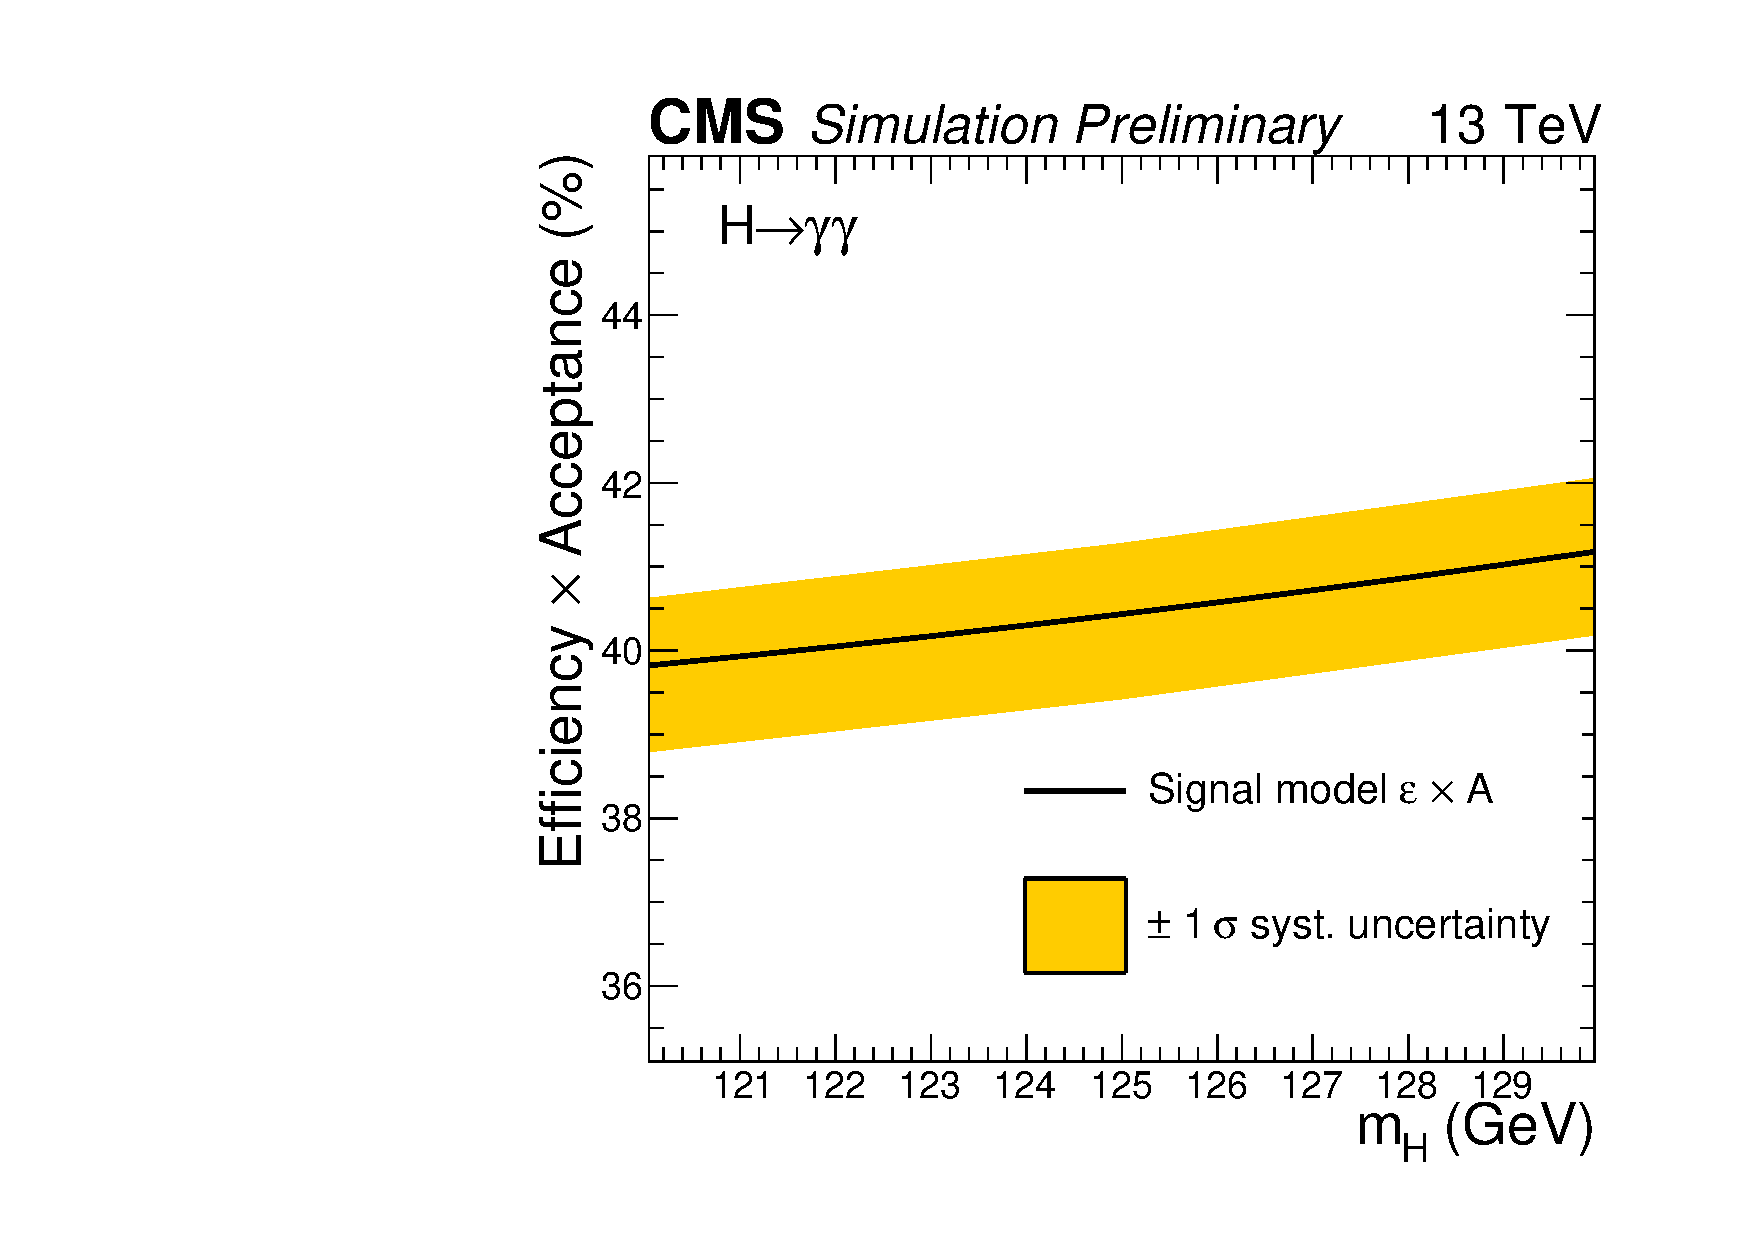
\includegraphics[width=0.7\textwidth]{modellingFigures/\whichFig/DCBpG/SSF/effAcc_vs_mass.pdf} 
\caption{The \effxacc of all categories combined shown as a function of \mH. The orange band shows the effect of the systematic uncertainties associated with trigger efficiency, photon identification and selection, photon energy scale and resolution, and vertex identification.}

\label{fig:model:sig_effxacc}
\end{figure}

The final normalisation of the signal models for an arbitrary value of \mH can then be obtained from the parametrised \effxacc multiplied by the relevant \crosssection, branching fraction and integrated luminosity.
As an example, the dependence of the full normalised parametric signal model on \mH for the \ggH process in each of the inclusive analysis categories is shown in \Fig~\ref{fig:model:sig_interpolation}. The equivalent figures for all processes in all categories are available in \App~\ref{app:modelling} in \Fig\s~\ref{fig:model:sig_interpolation_ggh}, ~\ref{fig:model:sig_interpolation_vbf}, ~\ref{fig:model:sig_interpolation_tth}, ~\ref{fig:model:sig_interpolation_wh}, and~\ref{fig:model:sig_interpolation_zh}.

\begin{figure}[htp!]
\centering
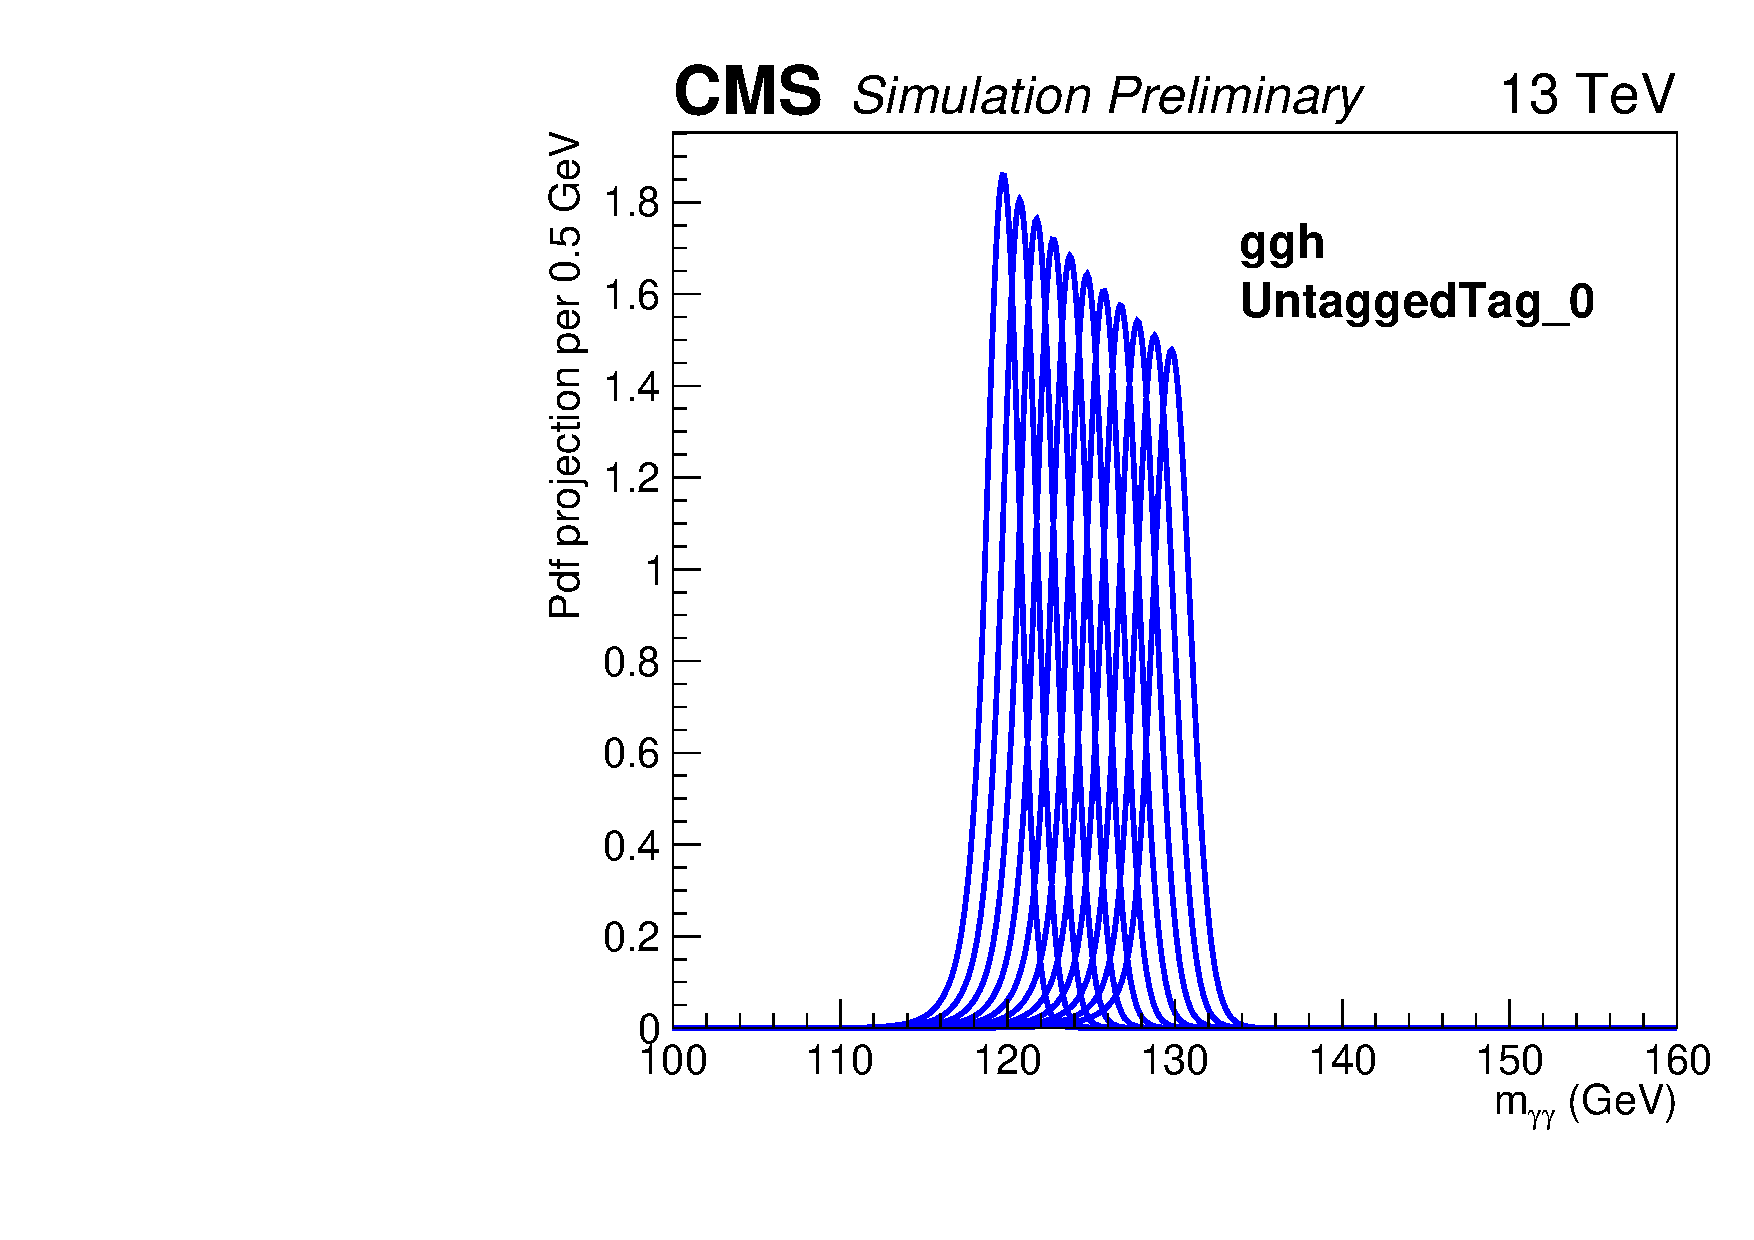
\includegraphics[width=0.47\textwidth]{modellingFigures/\whichFig/DCBpG/SSF/ggh_UntaggedTag_0_fmc_interp.pdf} 
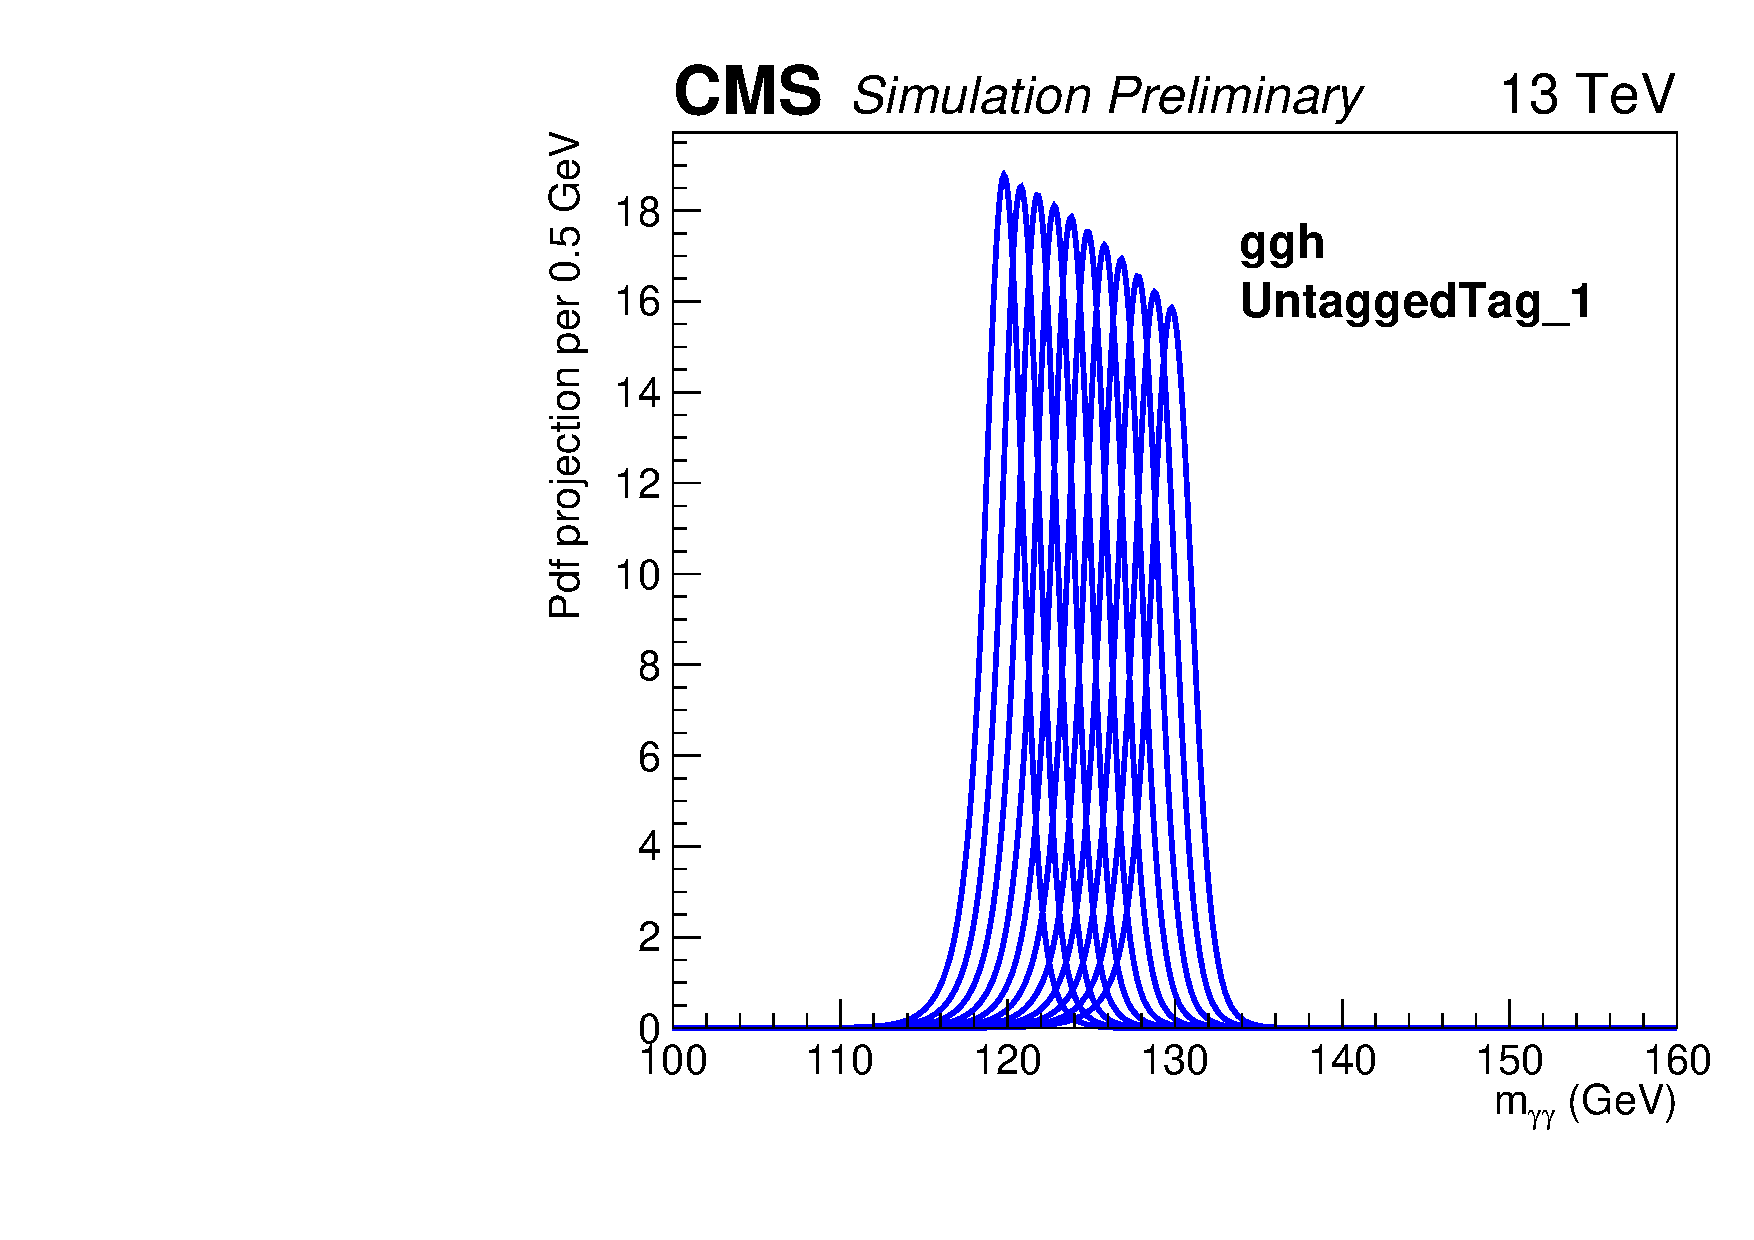
\includegraphics[width=0.47\textwidth]{modellingFigures/\whichFig/DCBpG/SSF/ggh_UntaggedTag_1_fmc_interp.pdf} \\ 
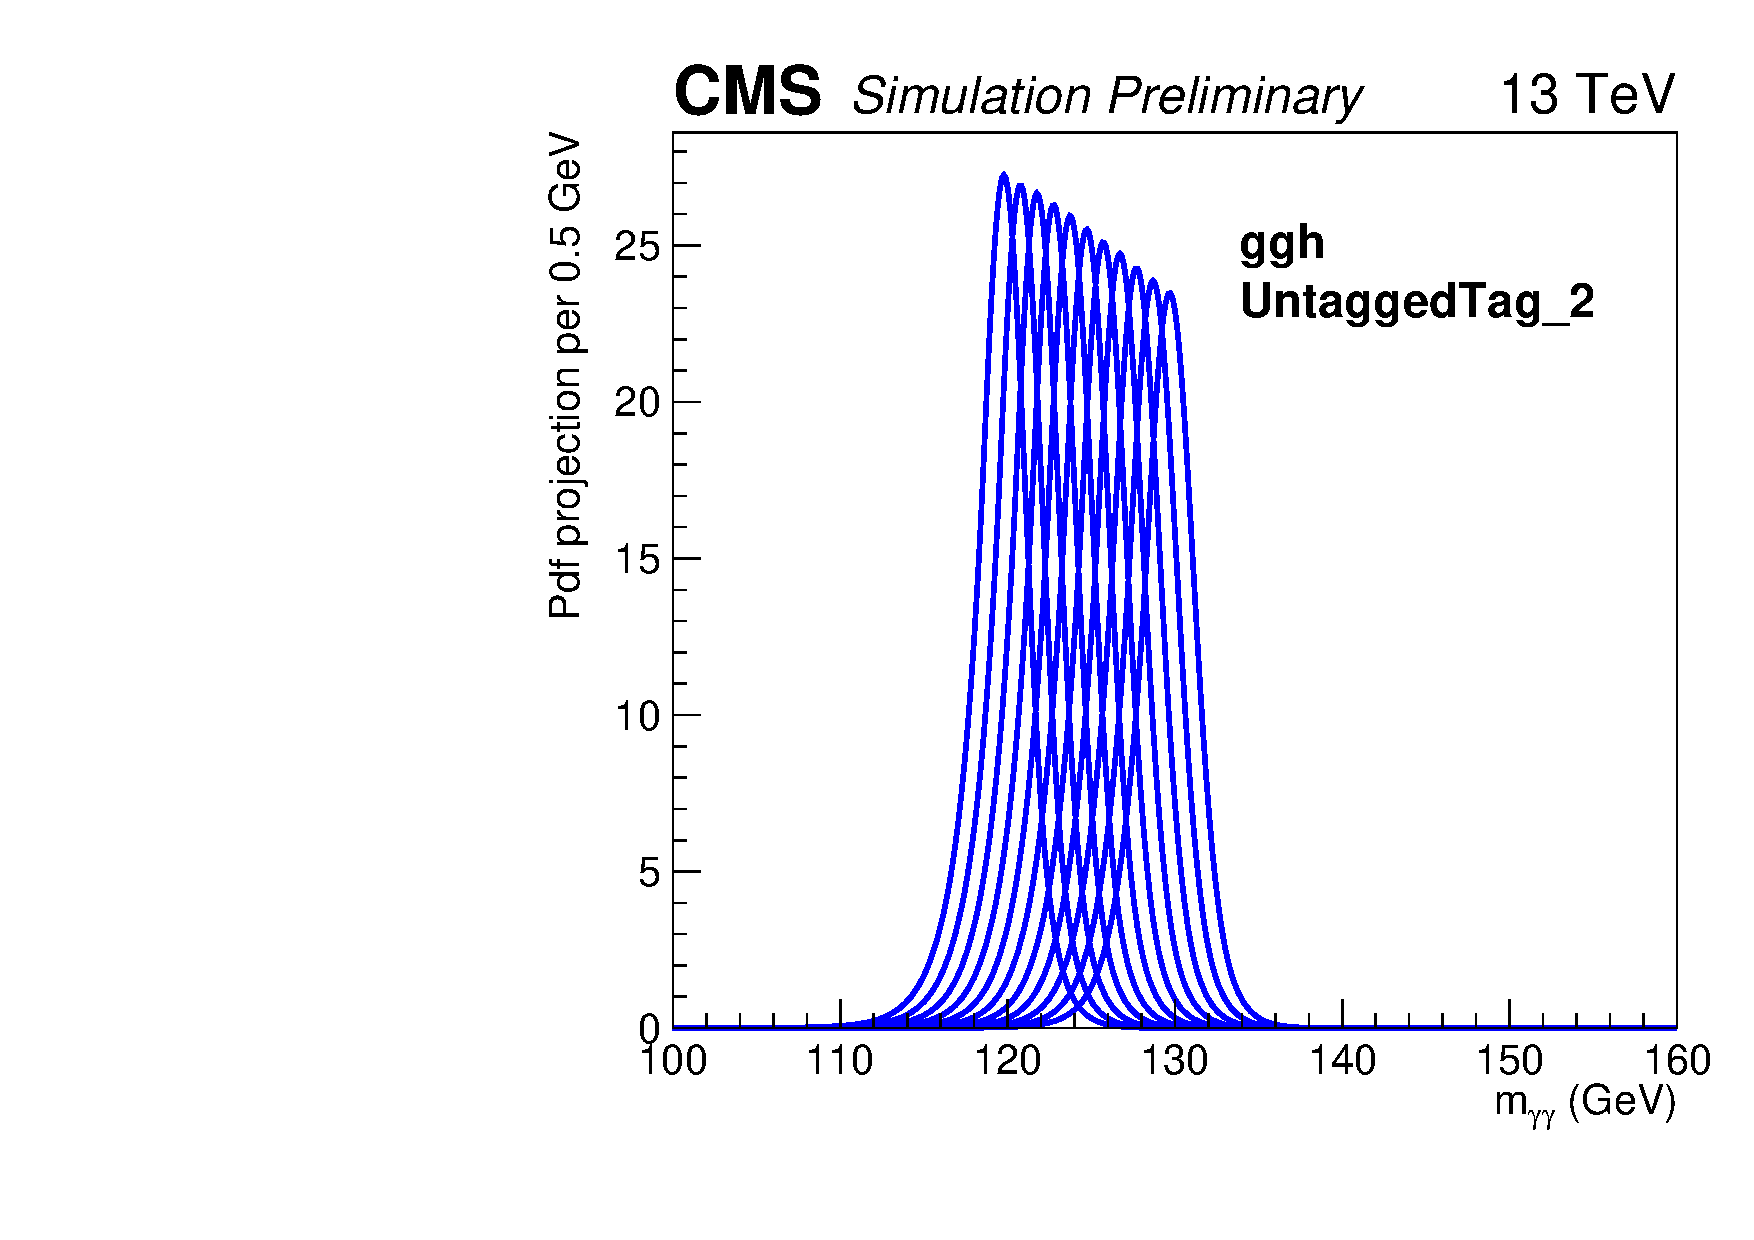
\includegraphics[width=0.47\textwidth]{modellingFigures/\whichFig/DCBpG/SSF/ggh_UntaggedTag_2_fmc_interp.pdf} 
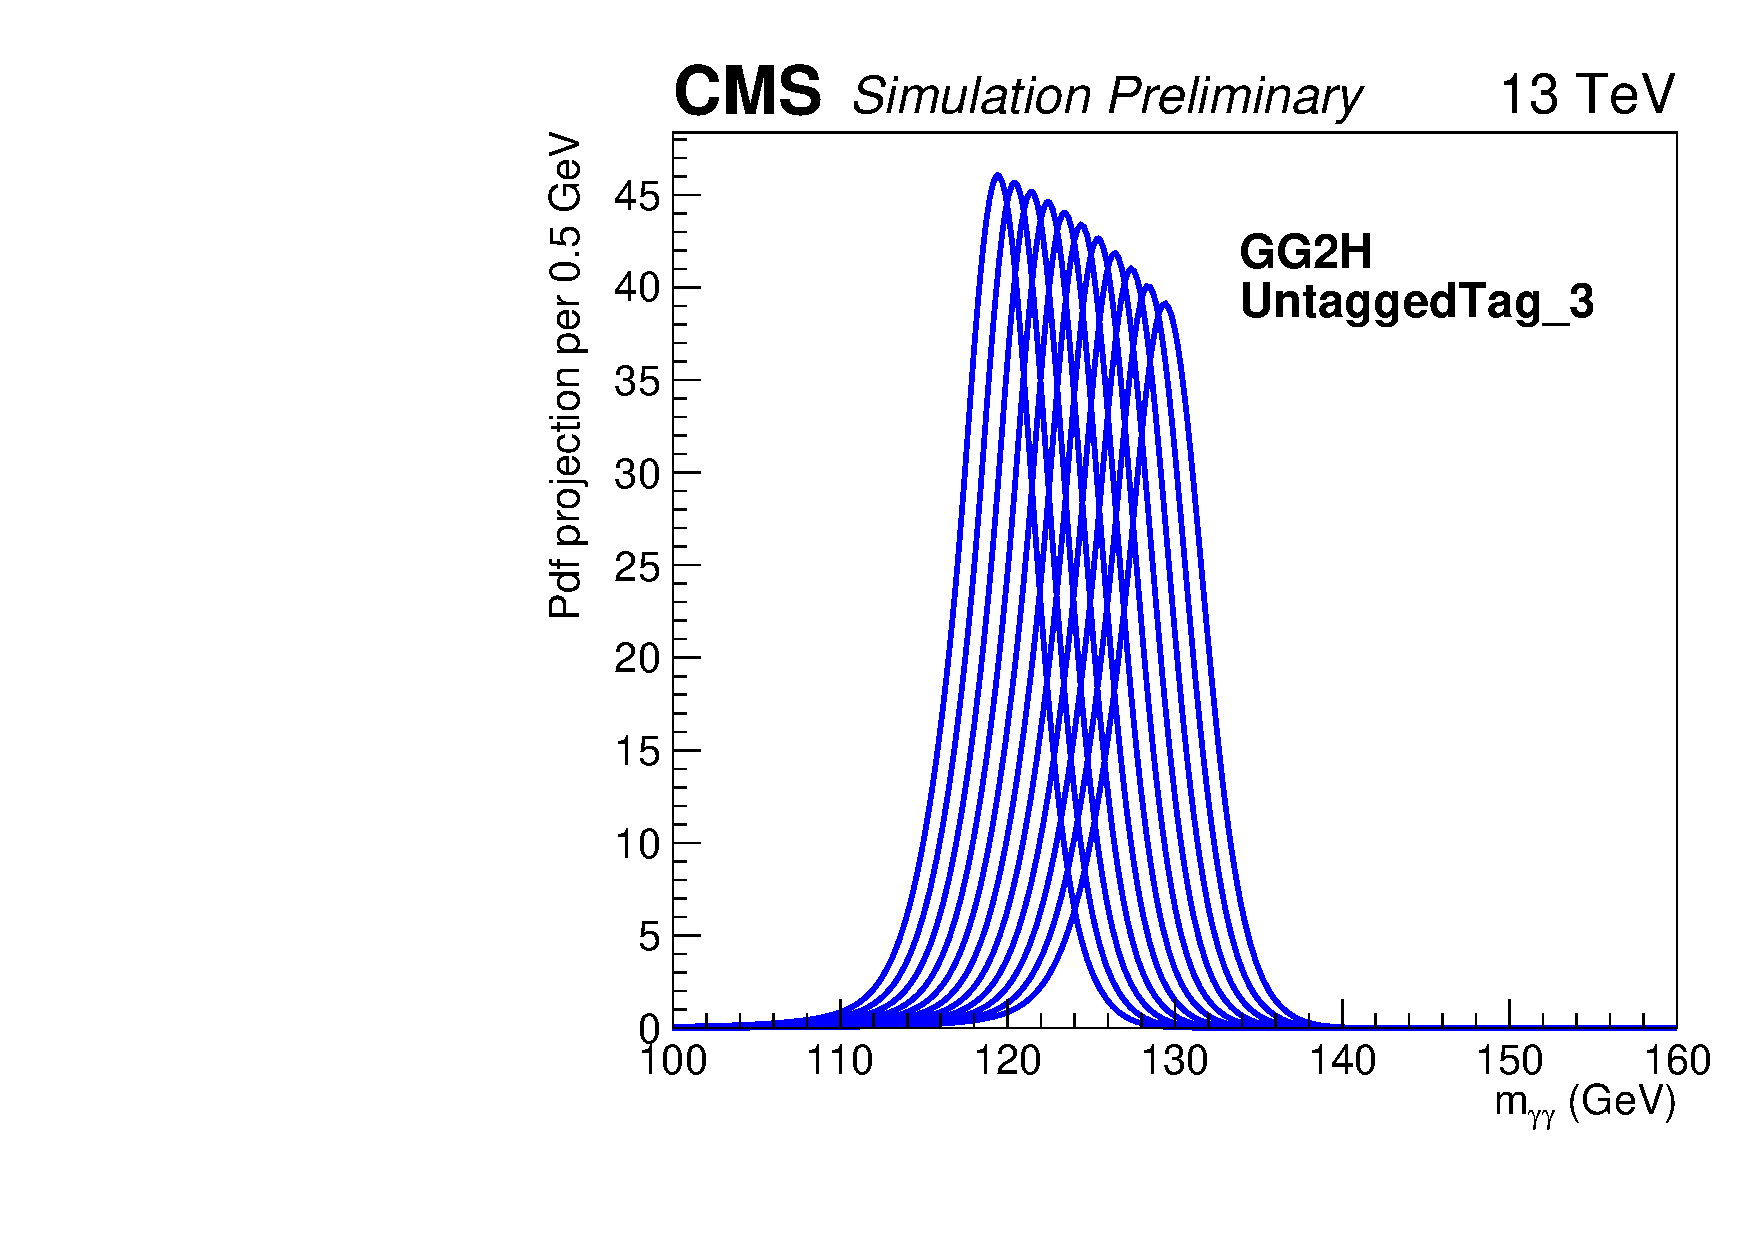
\includegraphics[width=0.47\textwidth]{modellingFigures/\whichFig/DCBpG/SSF/ggh_UntaggedTag_3_fmc_interp.pdf} \\
\caption{The \mH-dependence of the signal models for the ggH process for each of the \Untagged categories is shown. Each curve shows the signal model for a given value of \mH. The contributions from the RV and WV components of each model were interpolated between the samples for different \mH using the SSF method, and summed together according to their relative event content.}

\label{fig:model:sig_interpolation}
\end{figure}

%\begin{figure}[htp!]
%\centering
%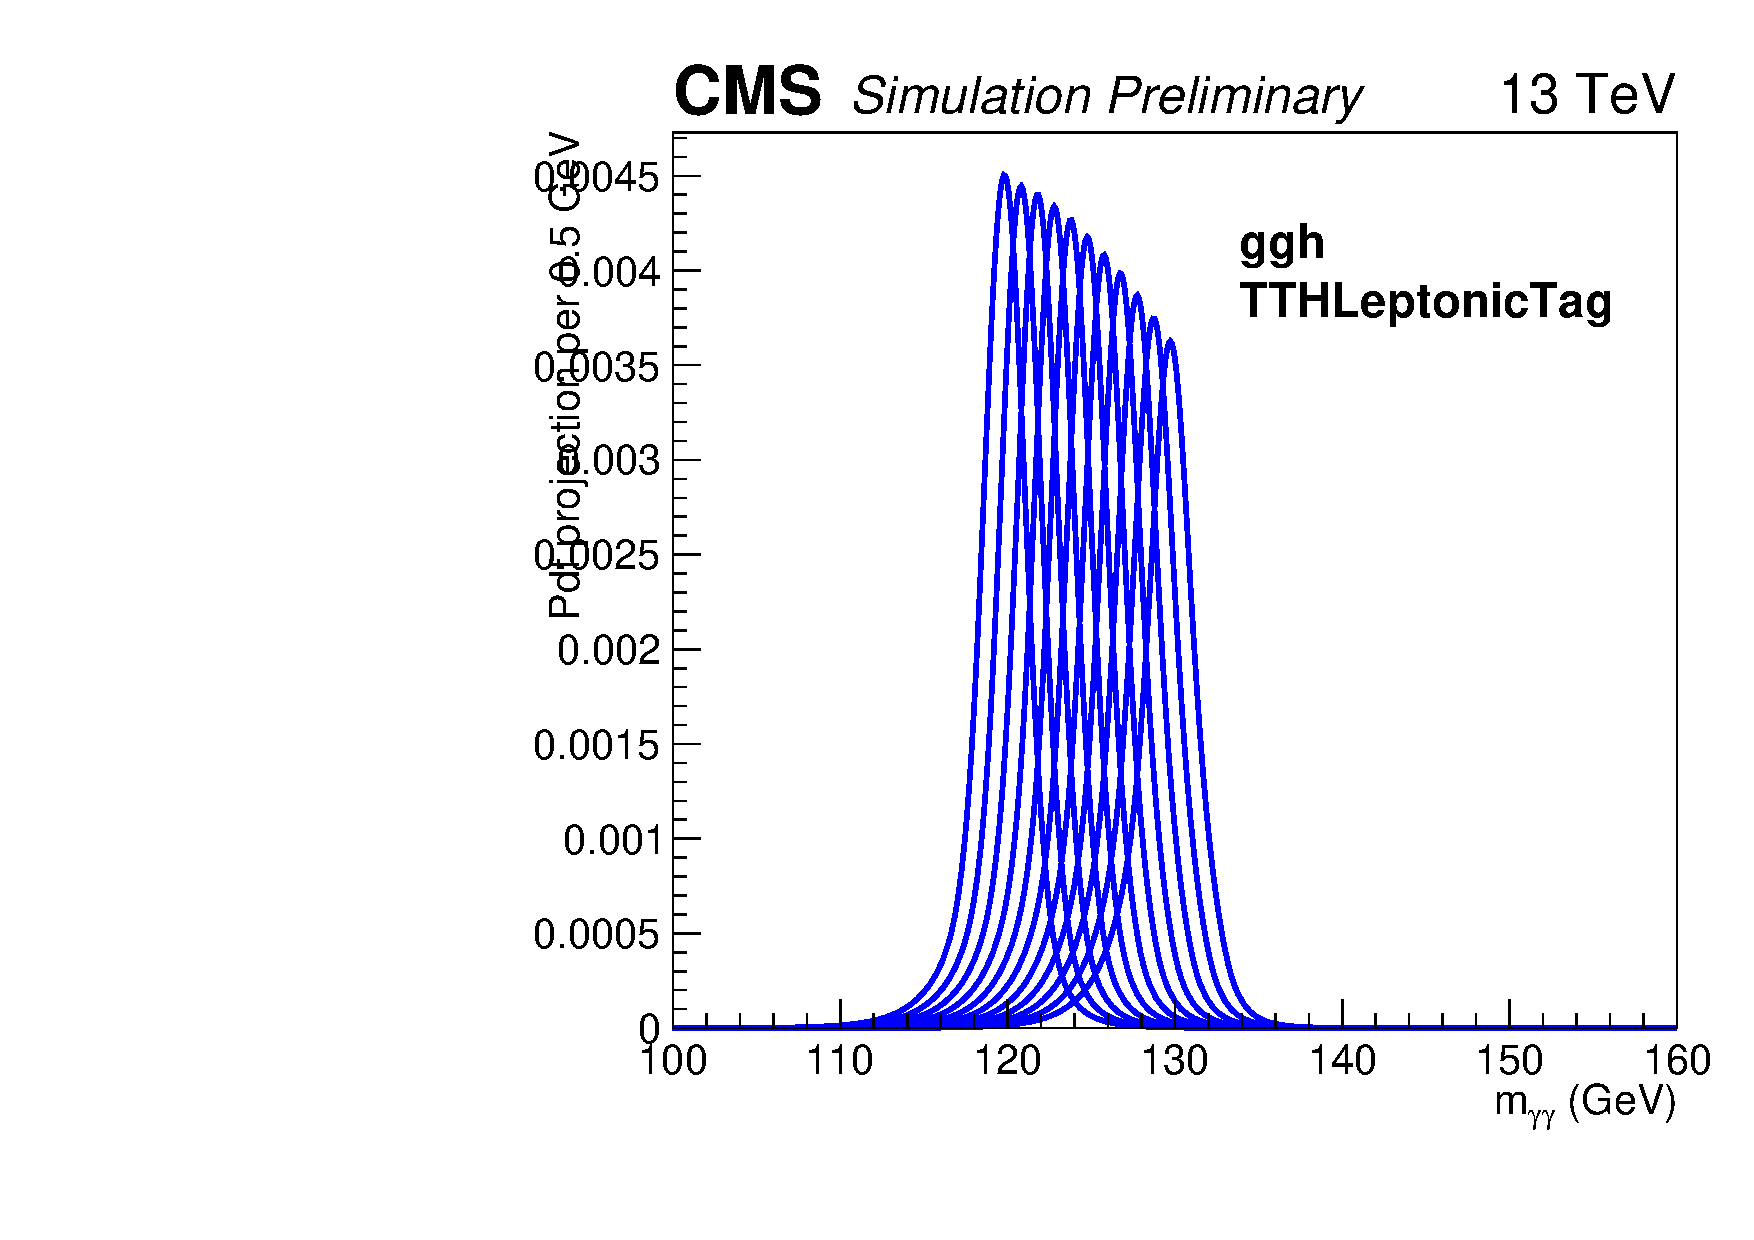
\includegraphics[width=0.47\textwidth]{modellingFigures/\whichFig/DCBpG/SSF/ggh_TTHLeptonicTag_fmc_interp.pdf} 
%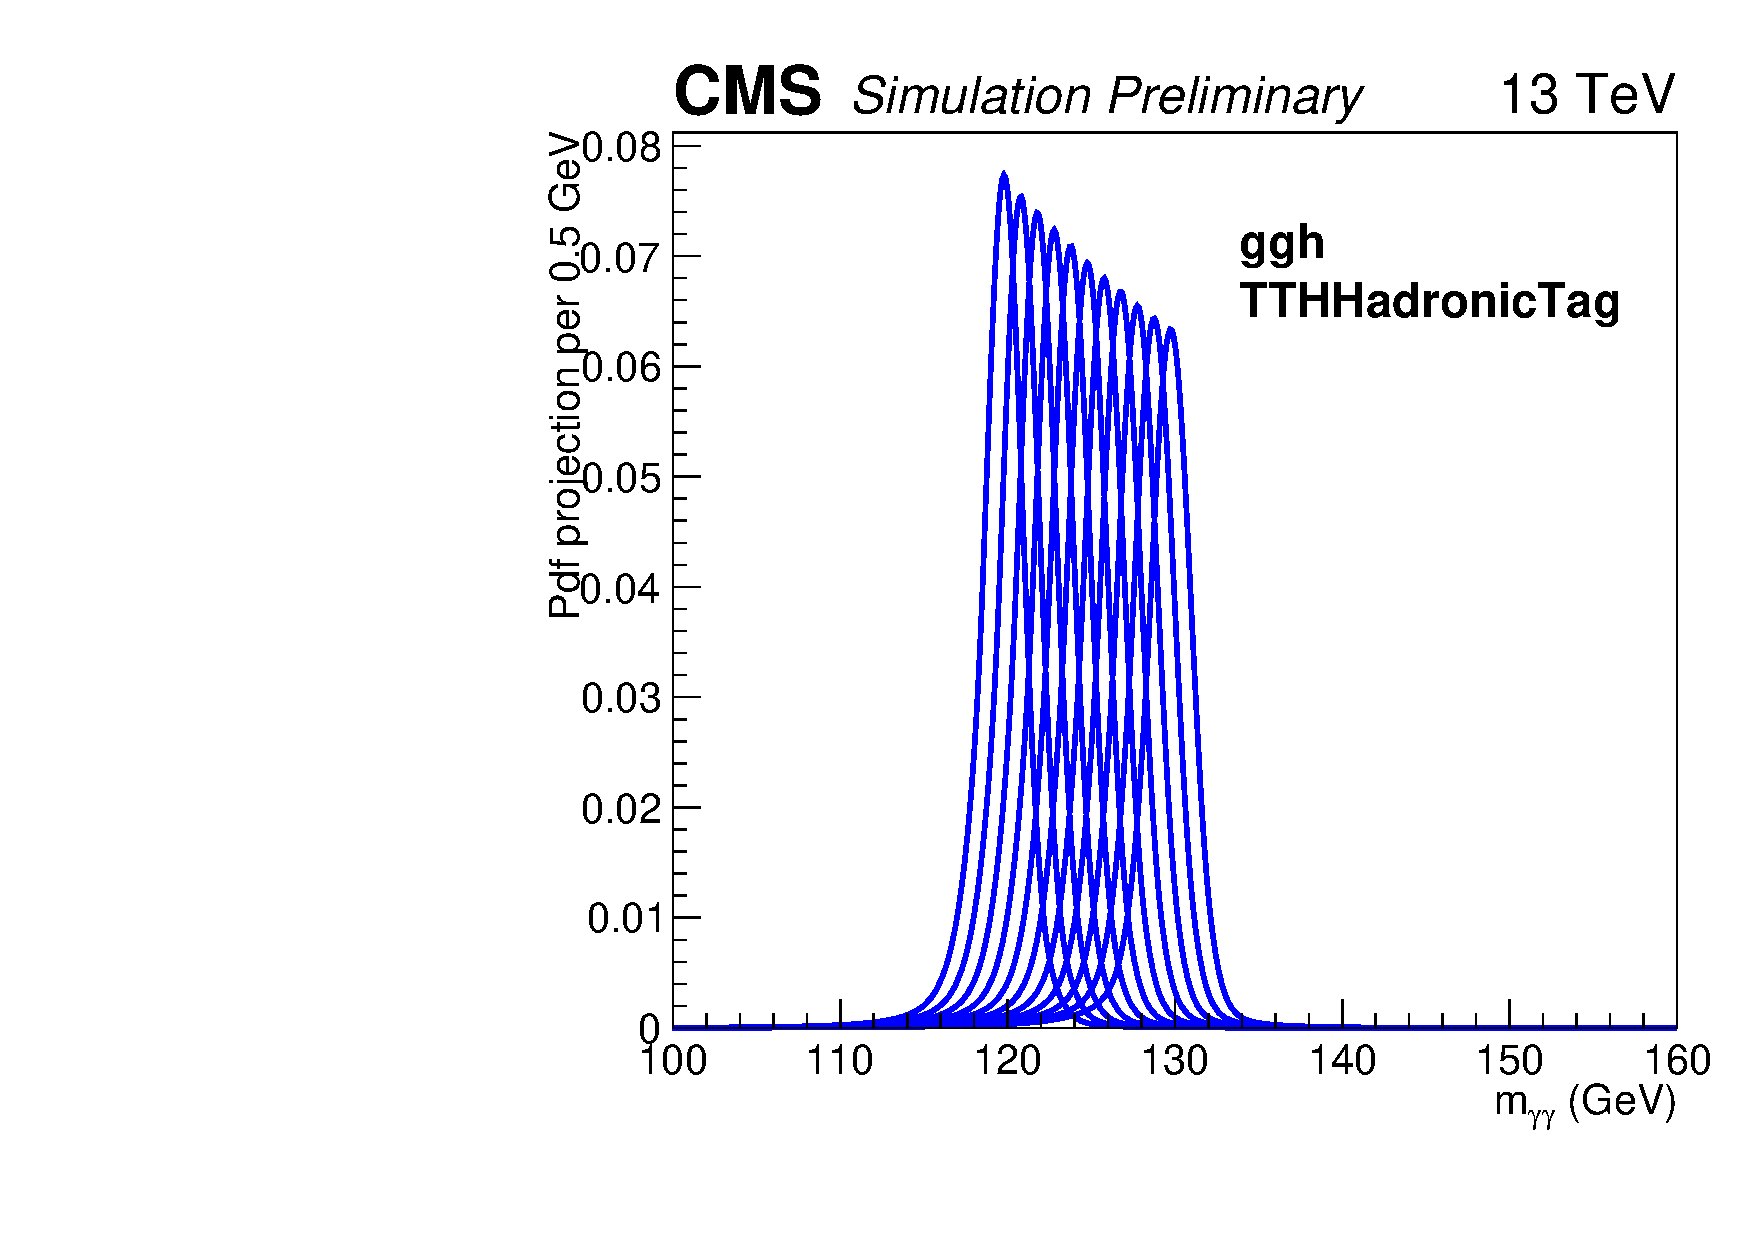
\includegraphics[width=0.47\textwidth]{modellingFigures/\whichFig/DCBpG/SSF/ggh_TTHHadronicTag_fmc_interp.pdf}\\ 
%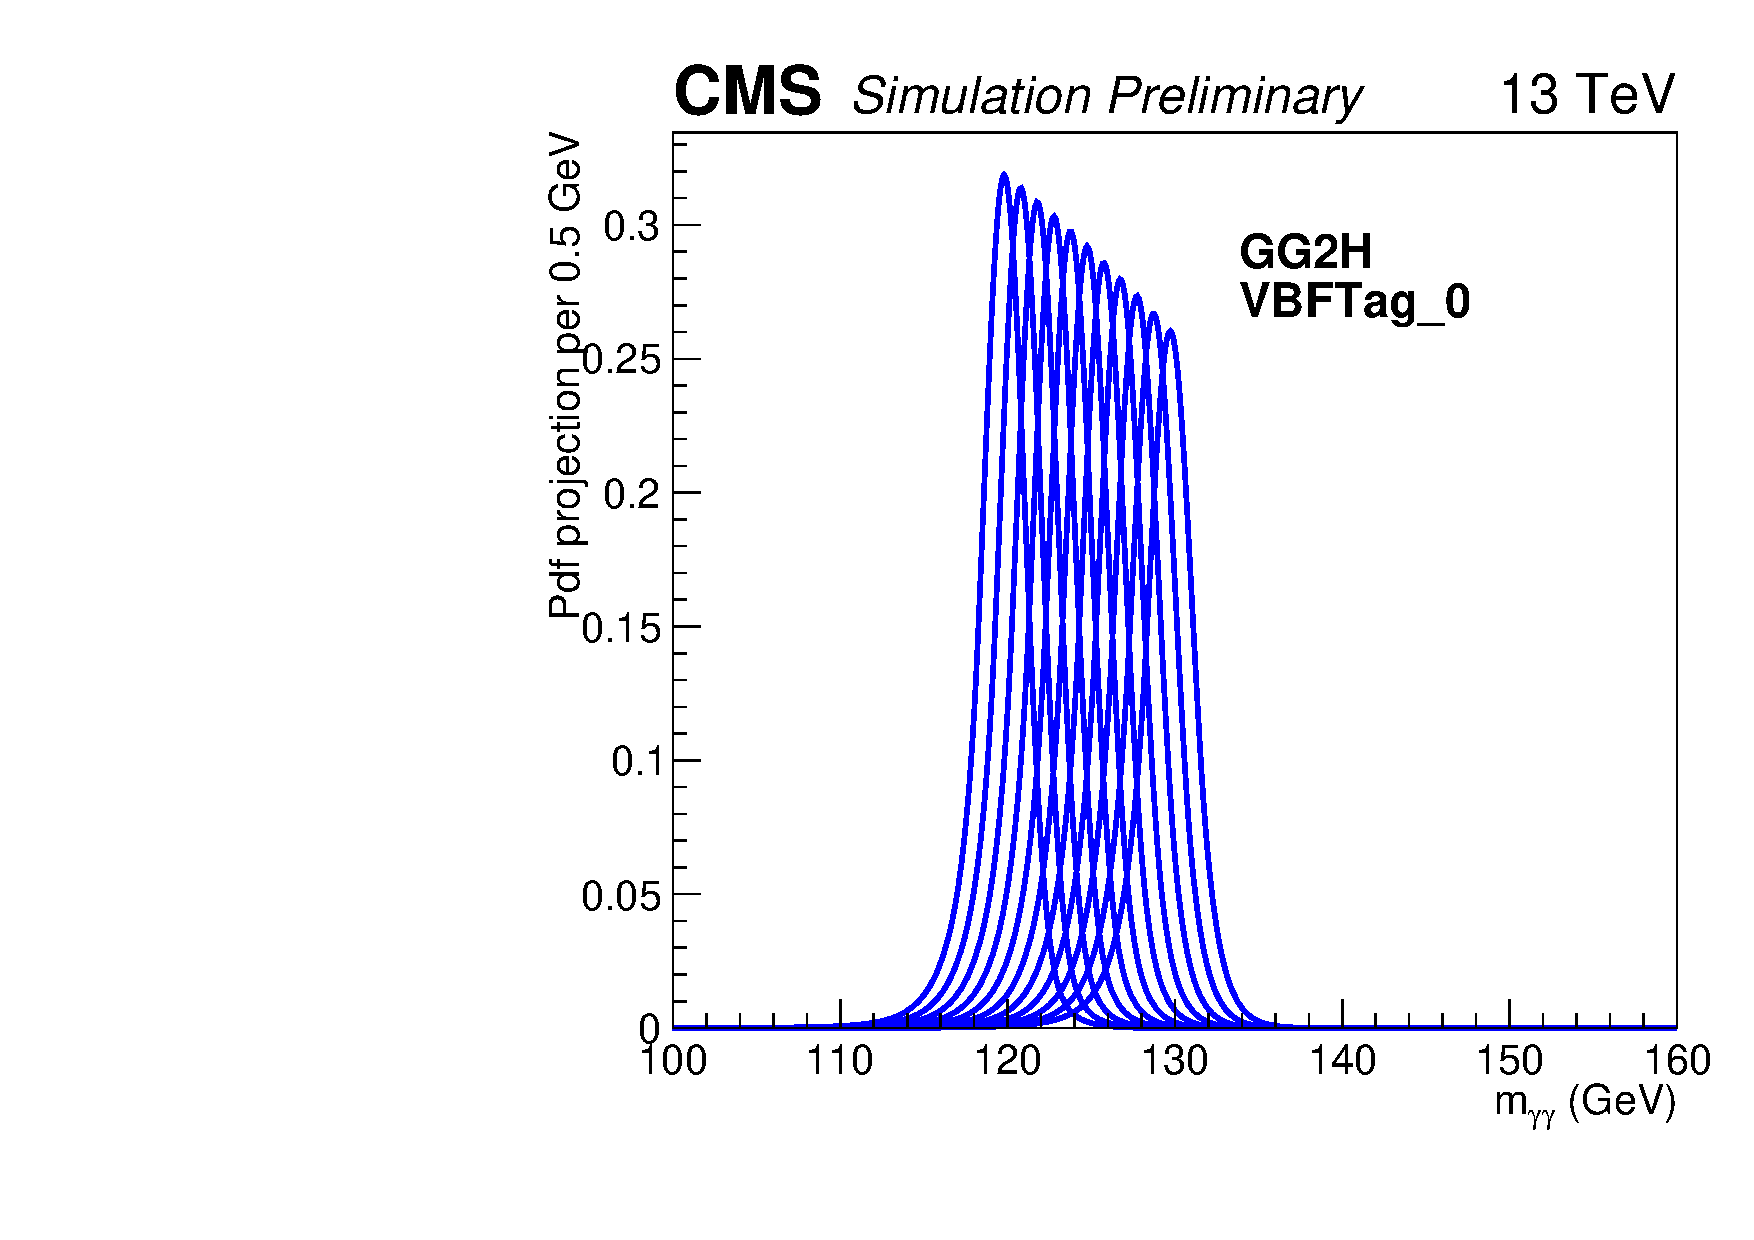
\includegraphics[width=0.47\textwidth]{modellingFigures/\whichFig/DCBpG/SSF/ggh_VBFTag_0_fmc_interp.pdf} 
%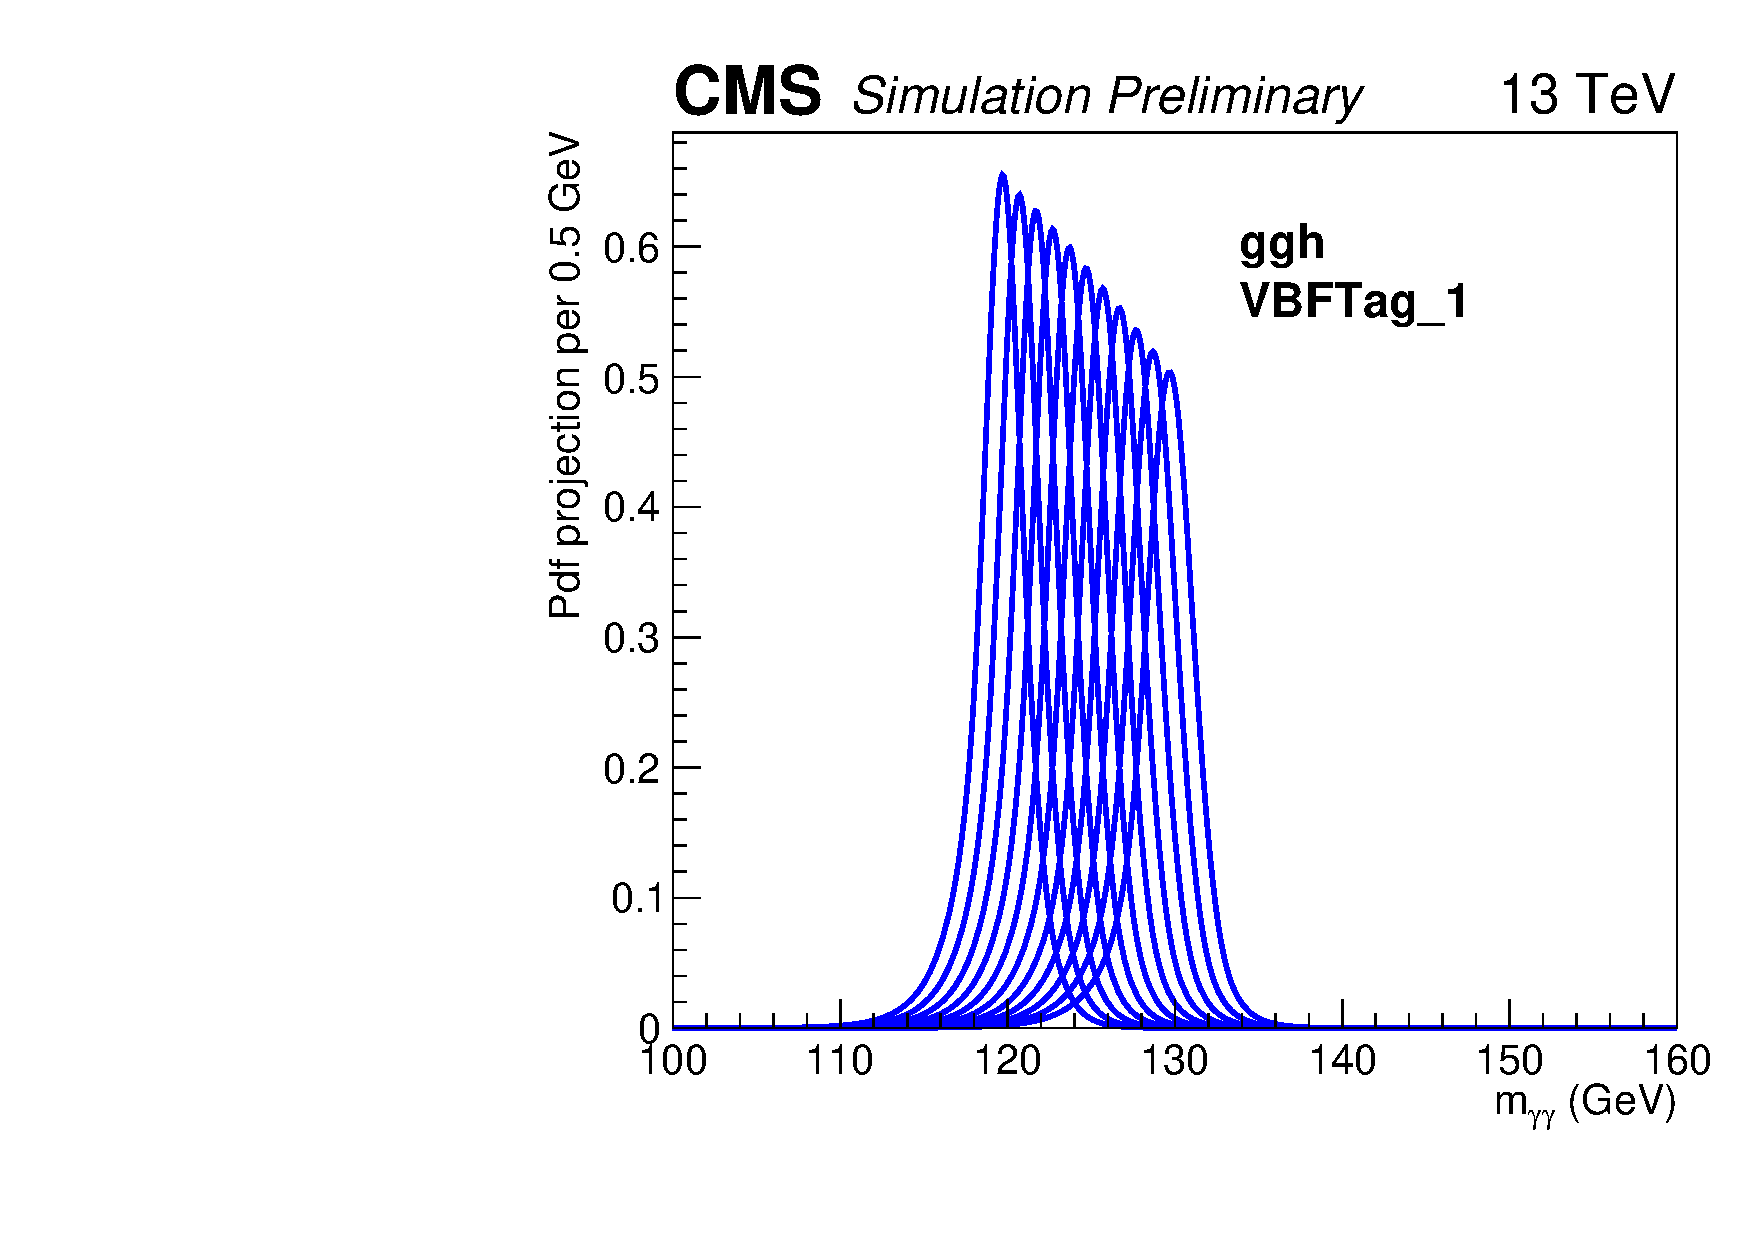
\includegraphics[width=0.47\textwidth]{modellingFigures/\whichFig/DCBpG/SSF/ggh_VBFTag_1_fmc_interp.pdf}\\ 
%\ifNewAnalysis 
%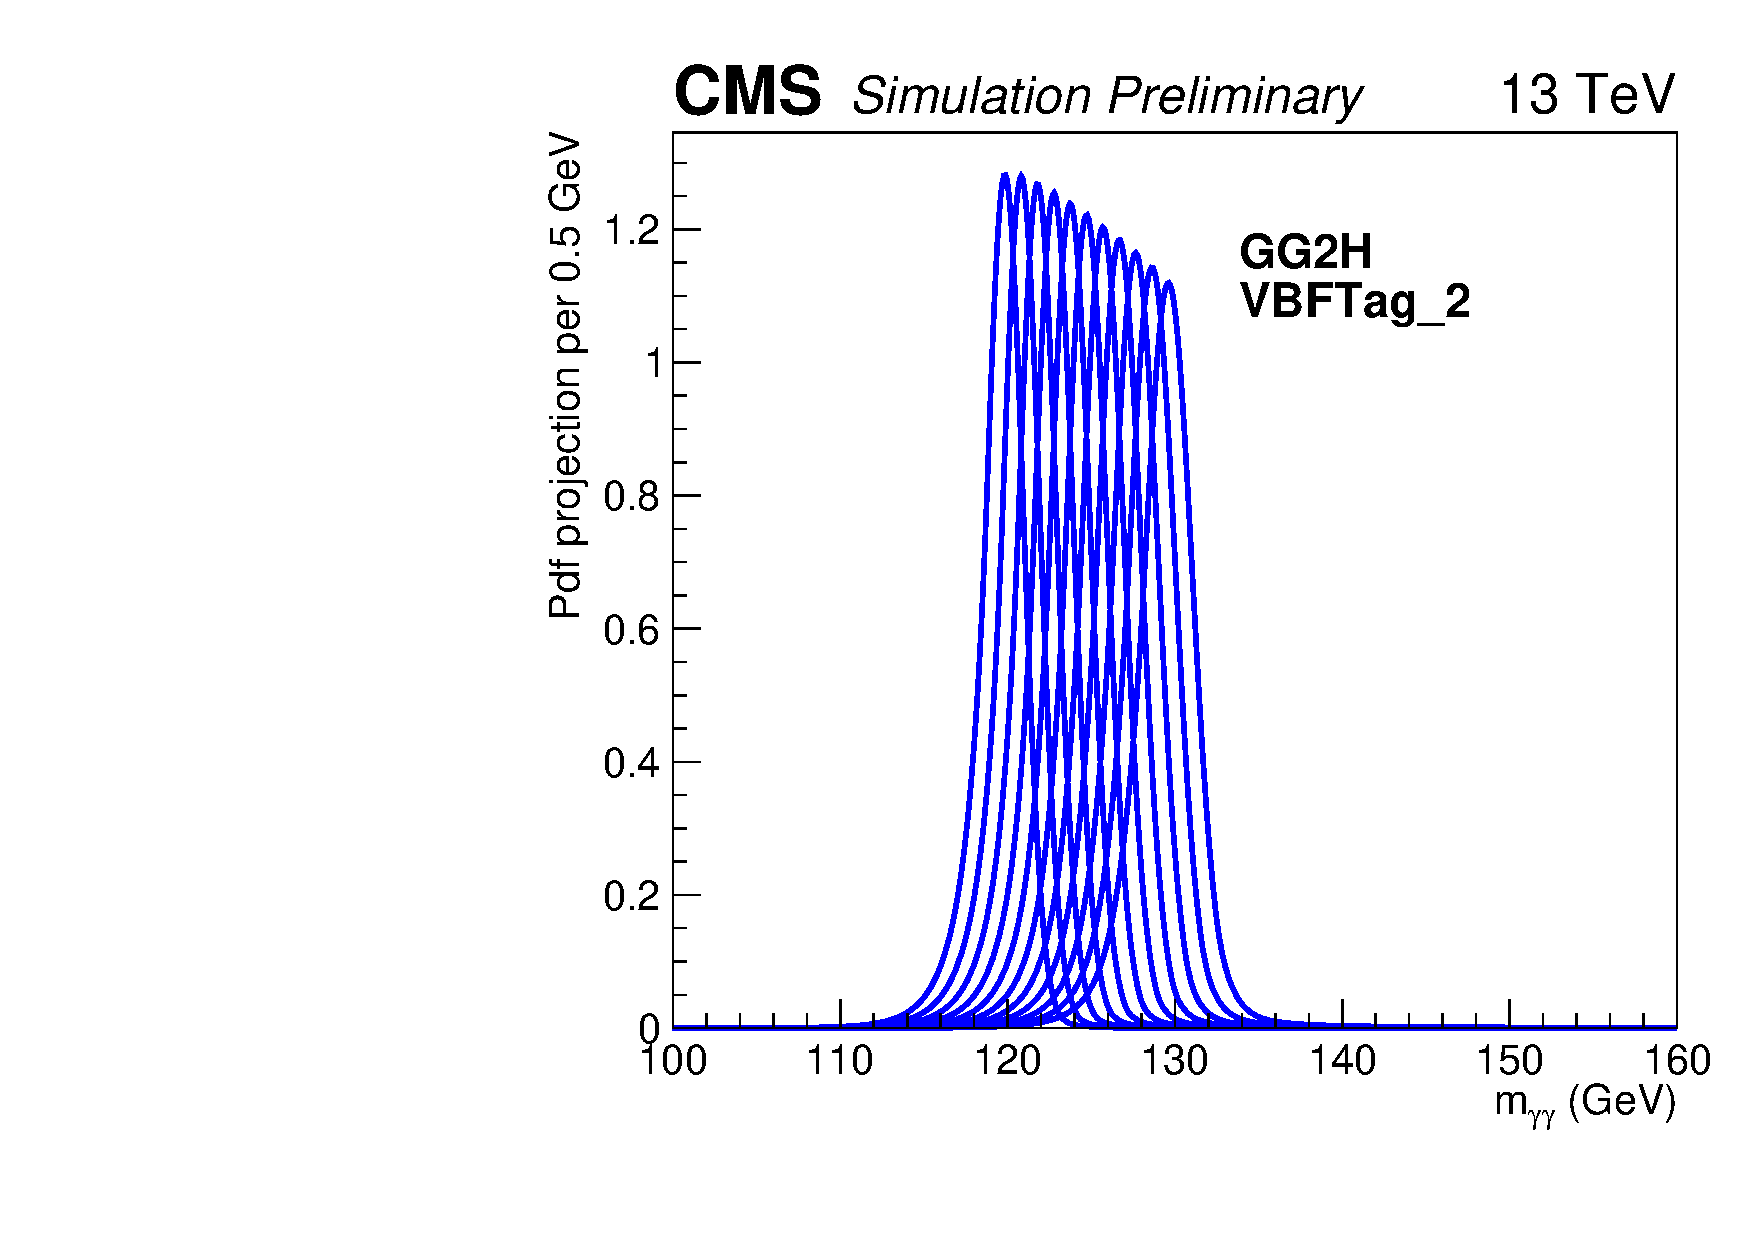
\includegraphics[width=0.47\textwidth]{modellingFigures/\whichFig/DCBpG/SSF/ggh_VBFTag_2_fmc_interp.pdf} 
%\fi
%\caption{The \mH-dependence of the signal models for the ggH process for each of \VBFTag and \TTHTag categories is shown. Each curve shows the signal model for a given value of \mH. The contributions from the RV and WV components of each model were summed together according to their relative size, and interpolated between the samples for different \mH using the SSF method.}
%
%\label{fig:model:sig_interpolation_bis}
%\end{figure}
%
%\ifNewAnalysis
%\begin{figure}[htp!]
%\centering
%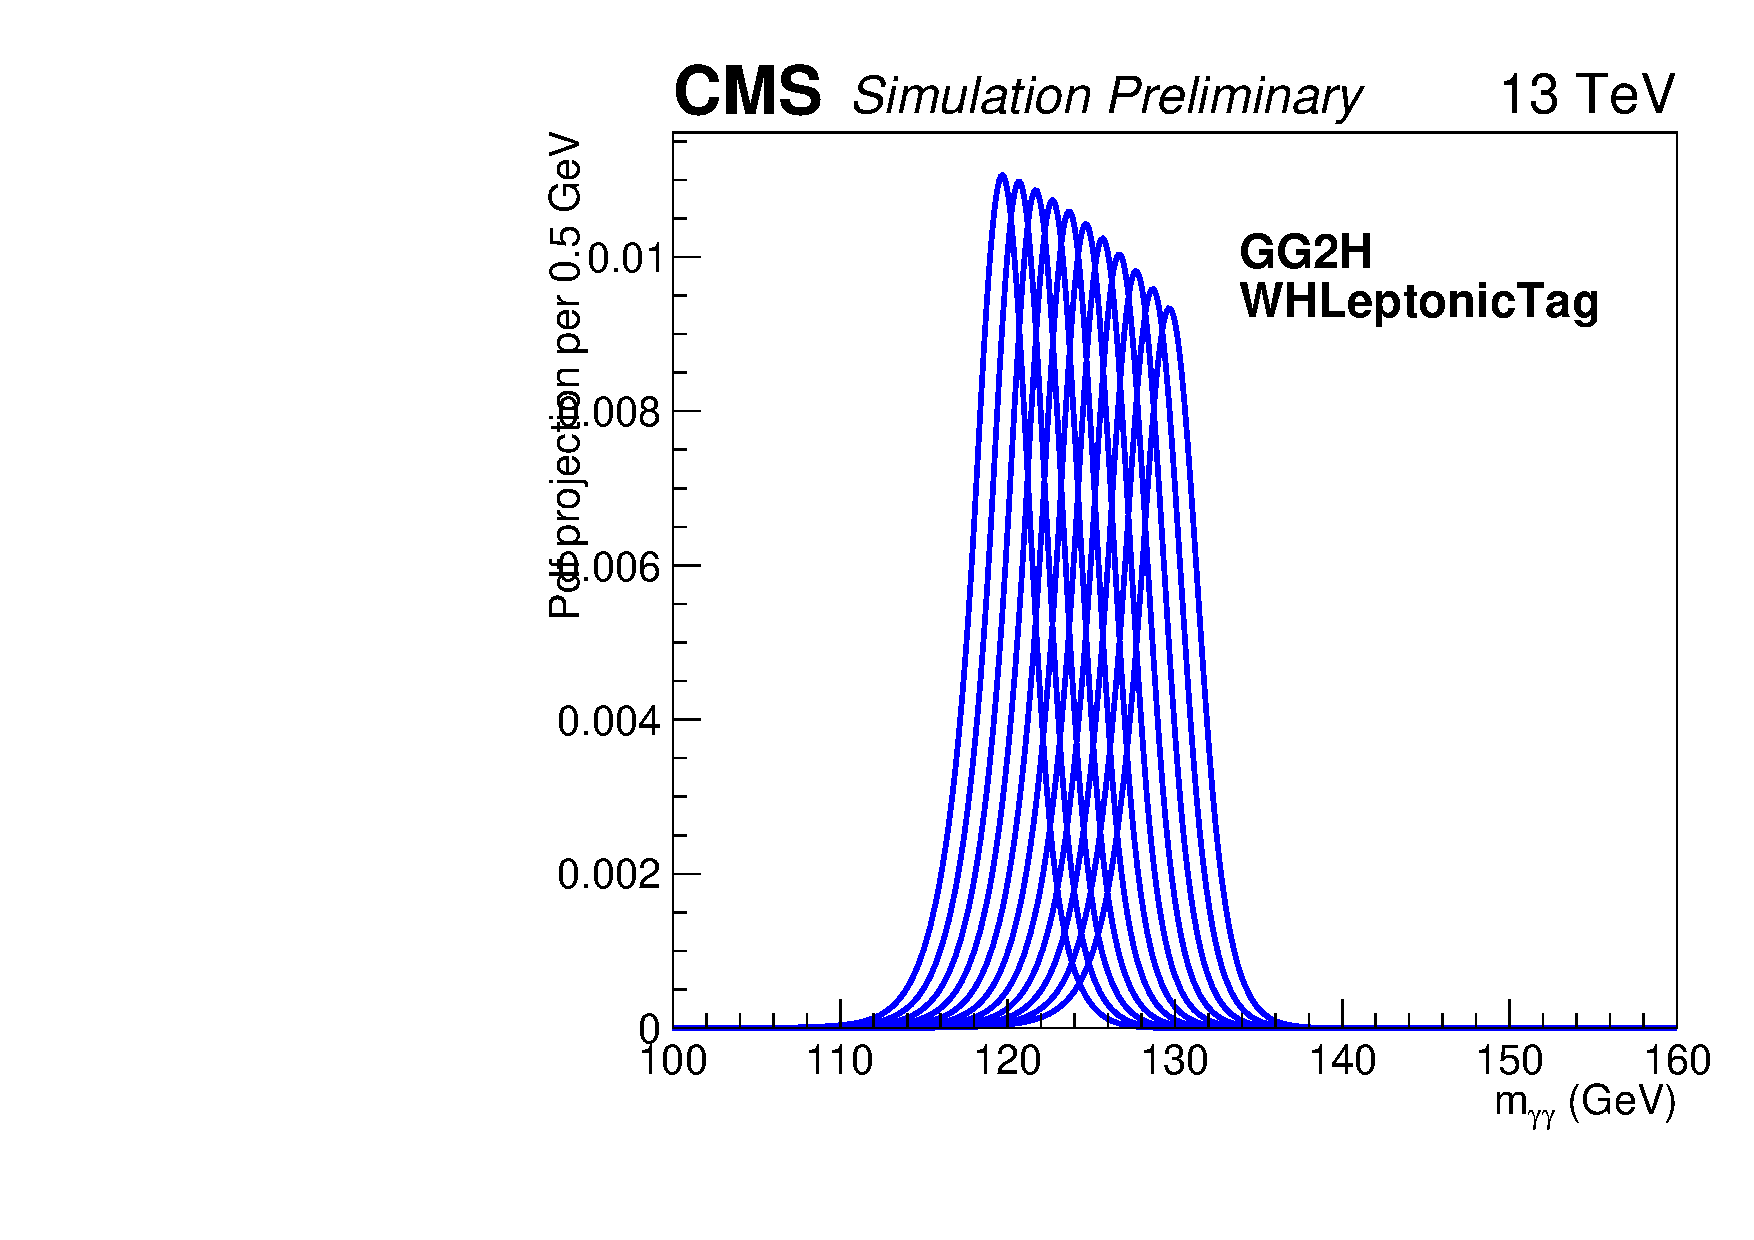
\includegraphics[width=0.47\textwidth]{modellingFigures/\whichFig/DCBpG/SSF/ggh_WHLeptonicTag_fmc_interp.pdf} 
%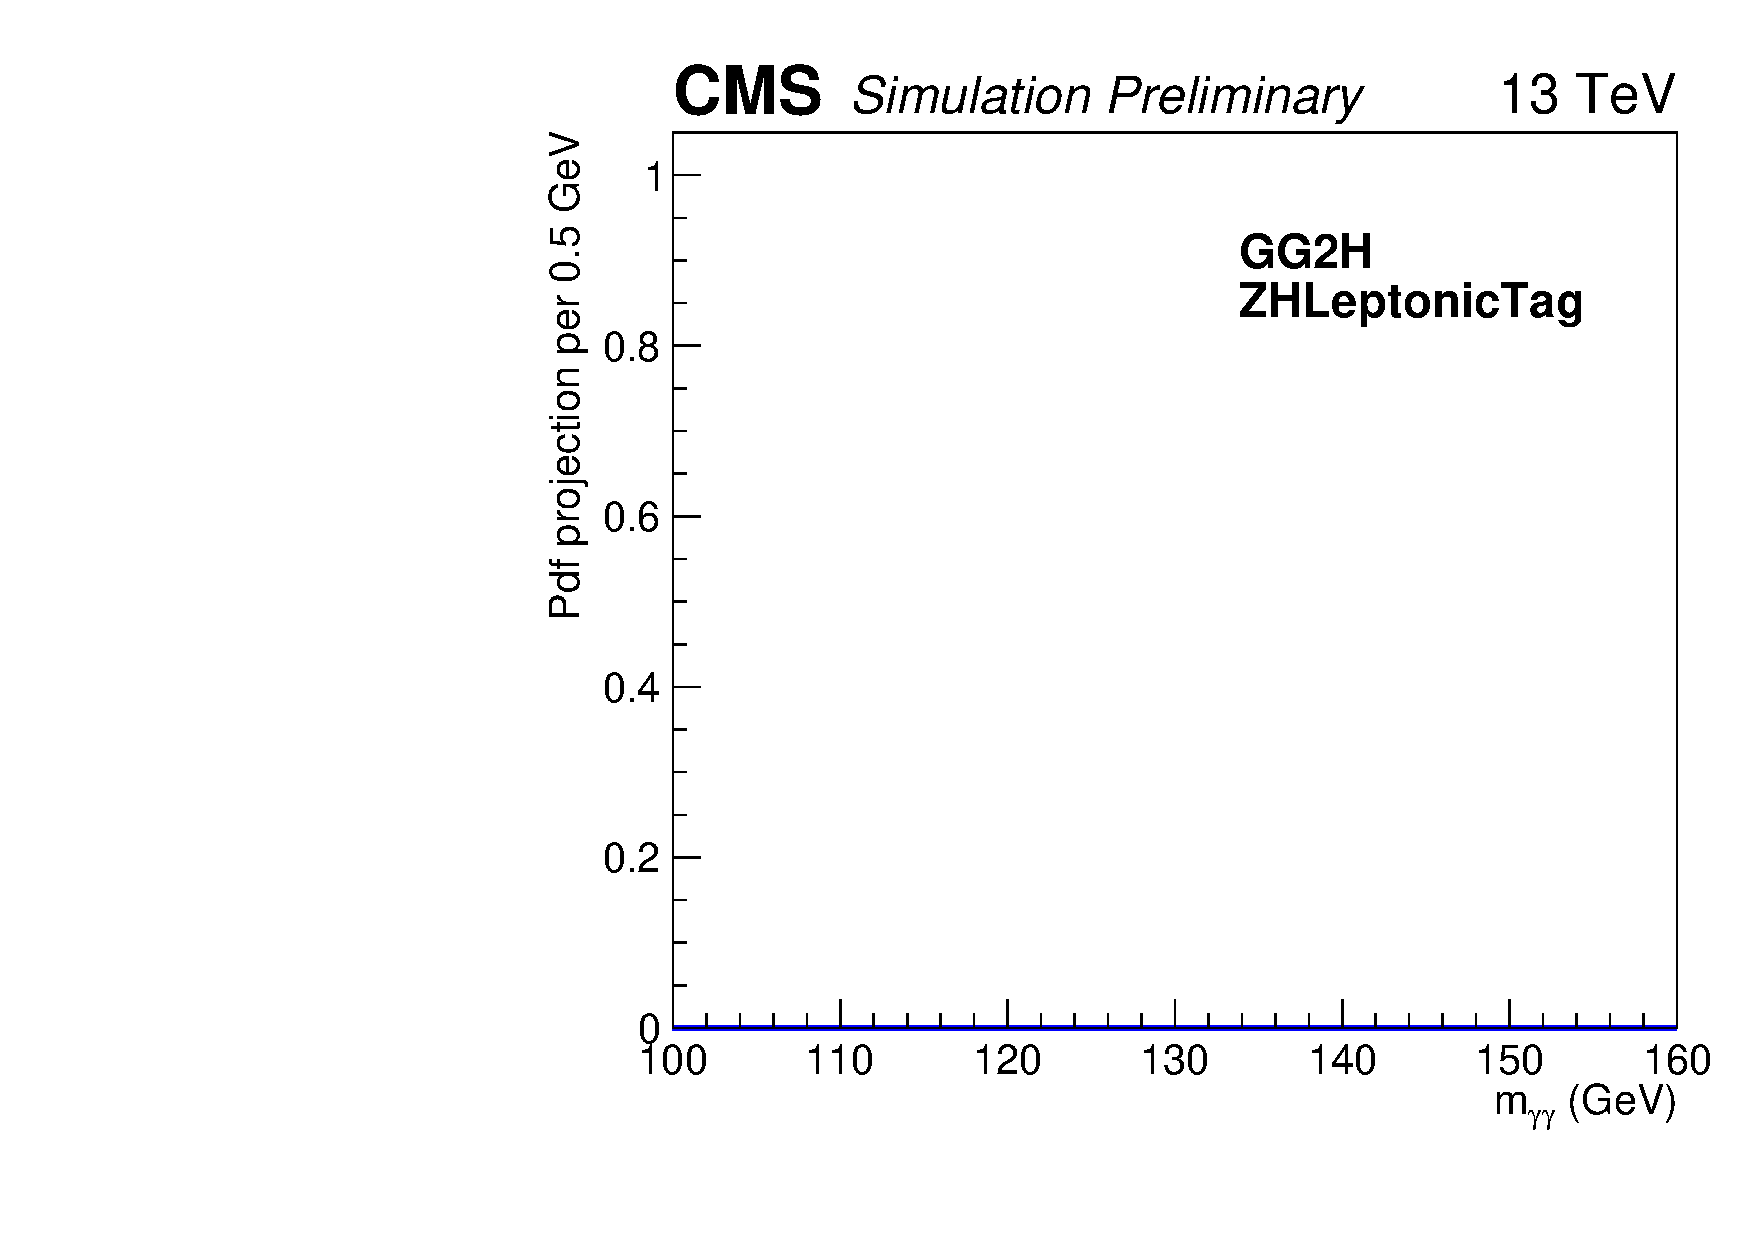
\includegraphics[width=0.47\textwidth]{modellingFigures/\whichFig/DCBpG/SSF/ggh_ZHLeptonicTag_fmc_interp.pdf} \\
%\includegraphics[width=0.47\textwidth]{modellingFigures/\whichFig/DCBpG/SSF/ggh_VHLeptoniclooseTag_fmc_interp.pdf} 
%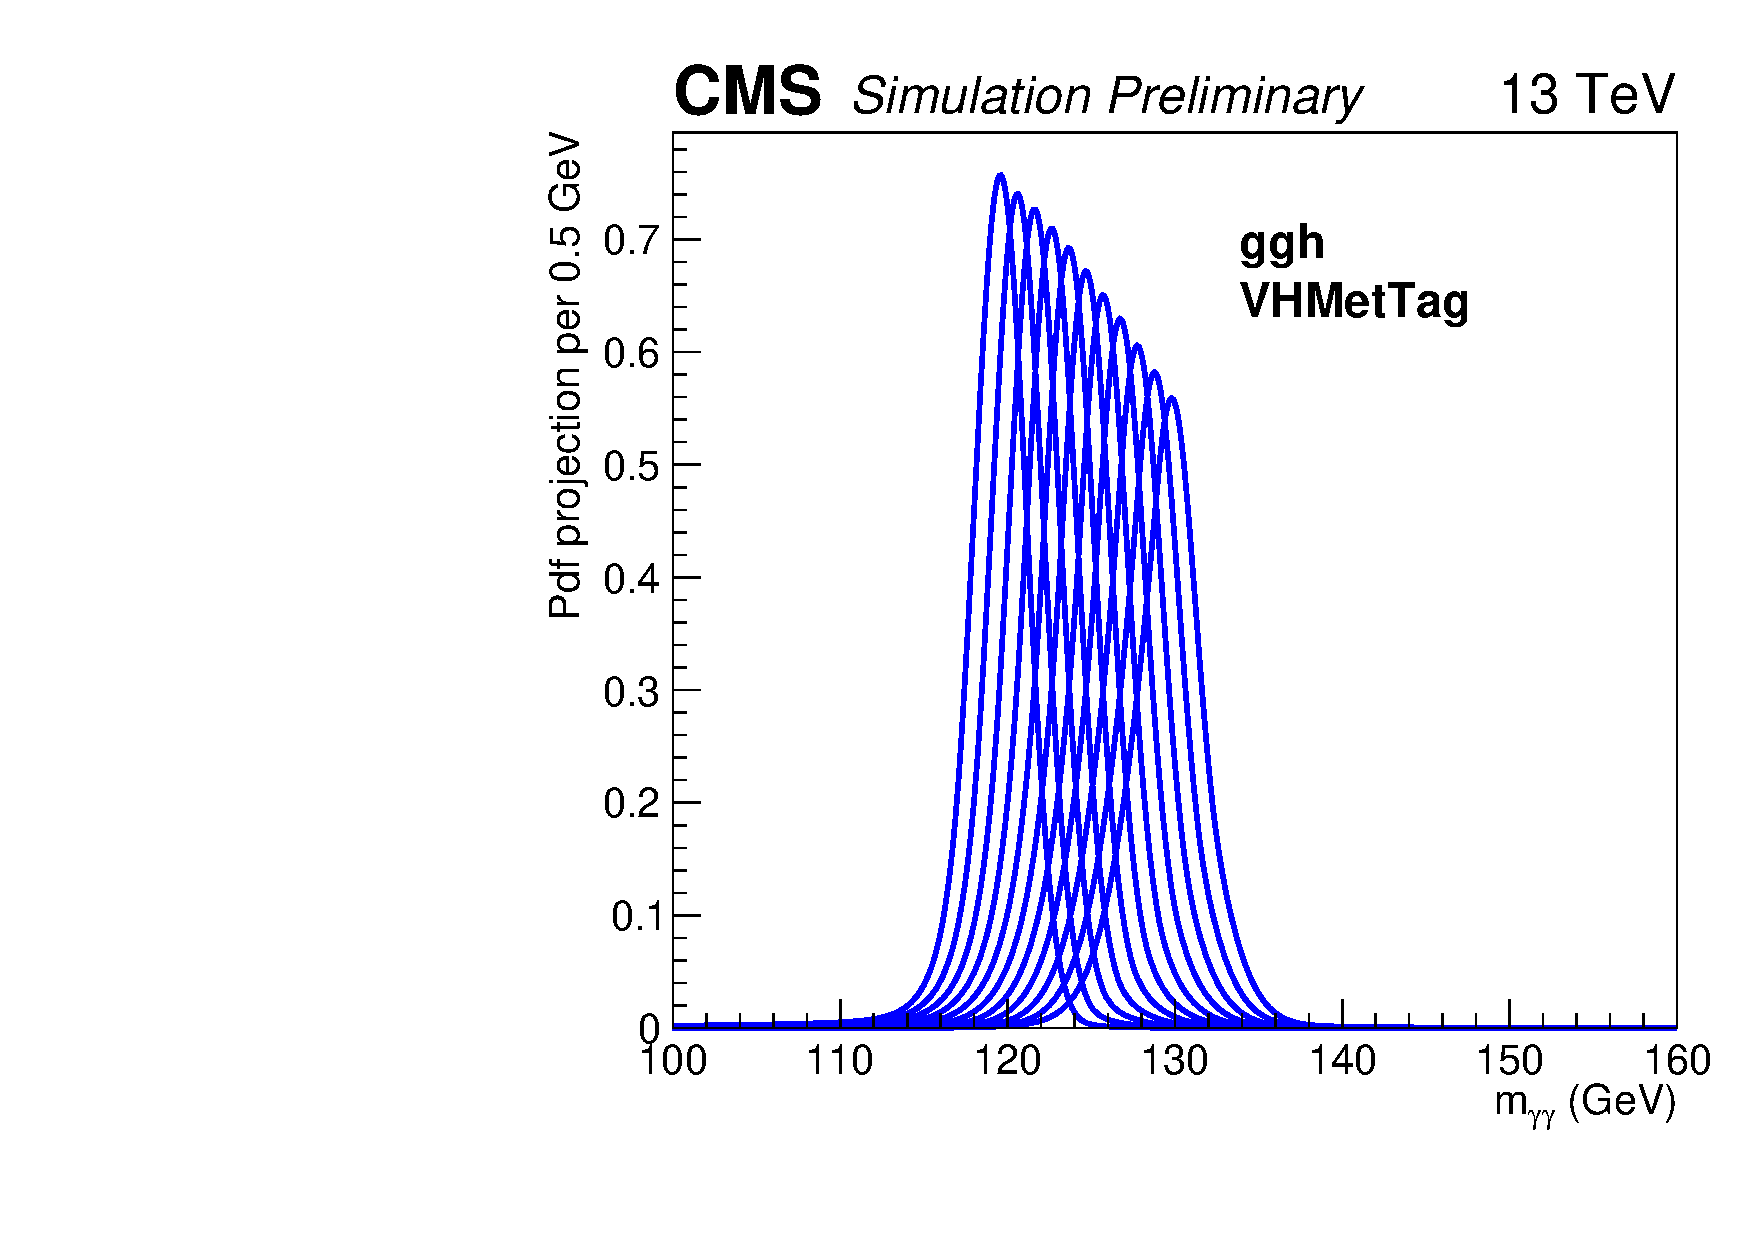
\includegraphics[width=0.47\textwidth]{modellingFigures/\whichFig/DCBpG/SSF/ggh_VHMetTag_fmc_interp.pdf} \\
%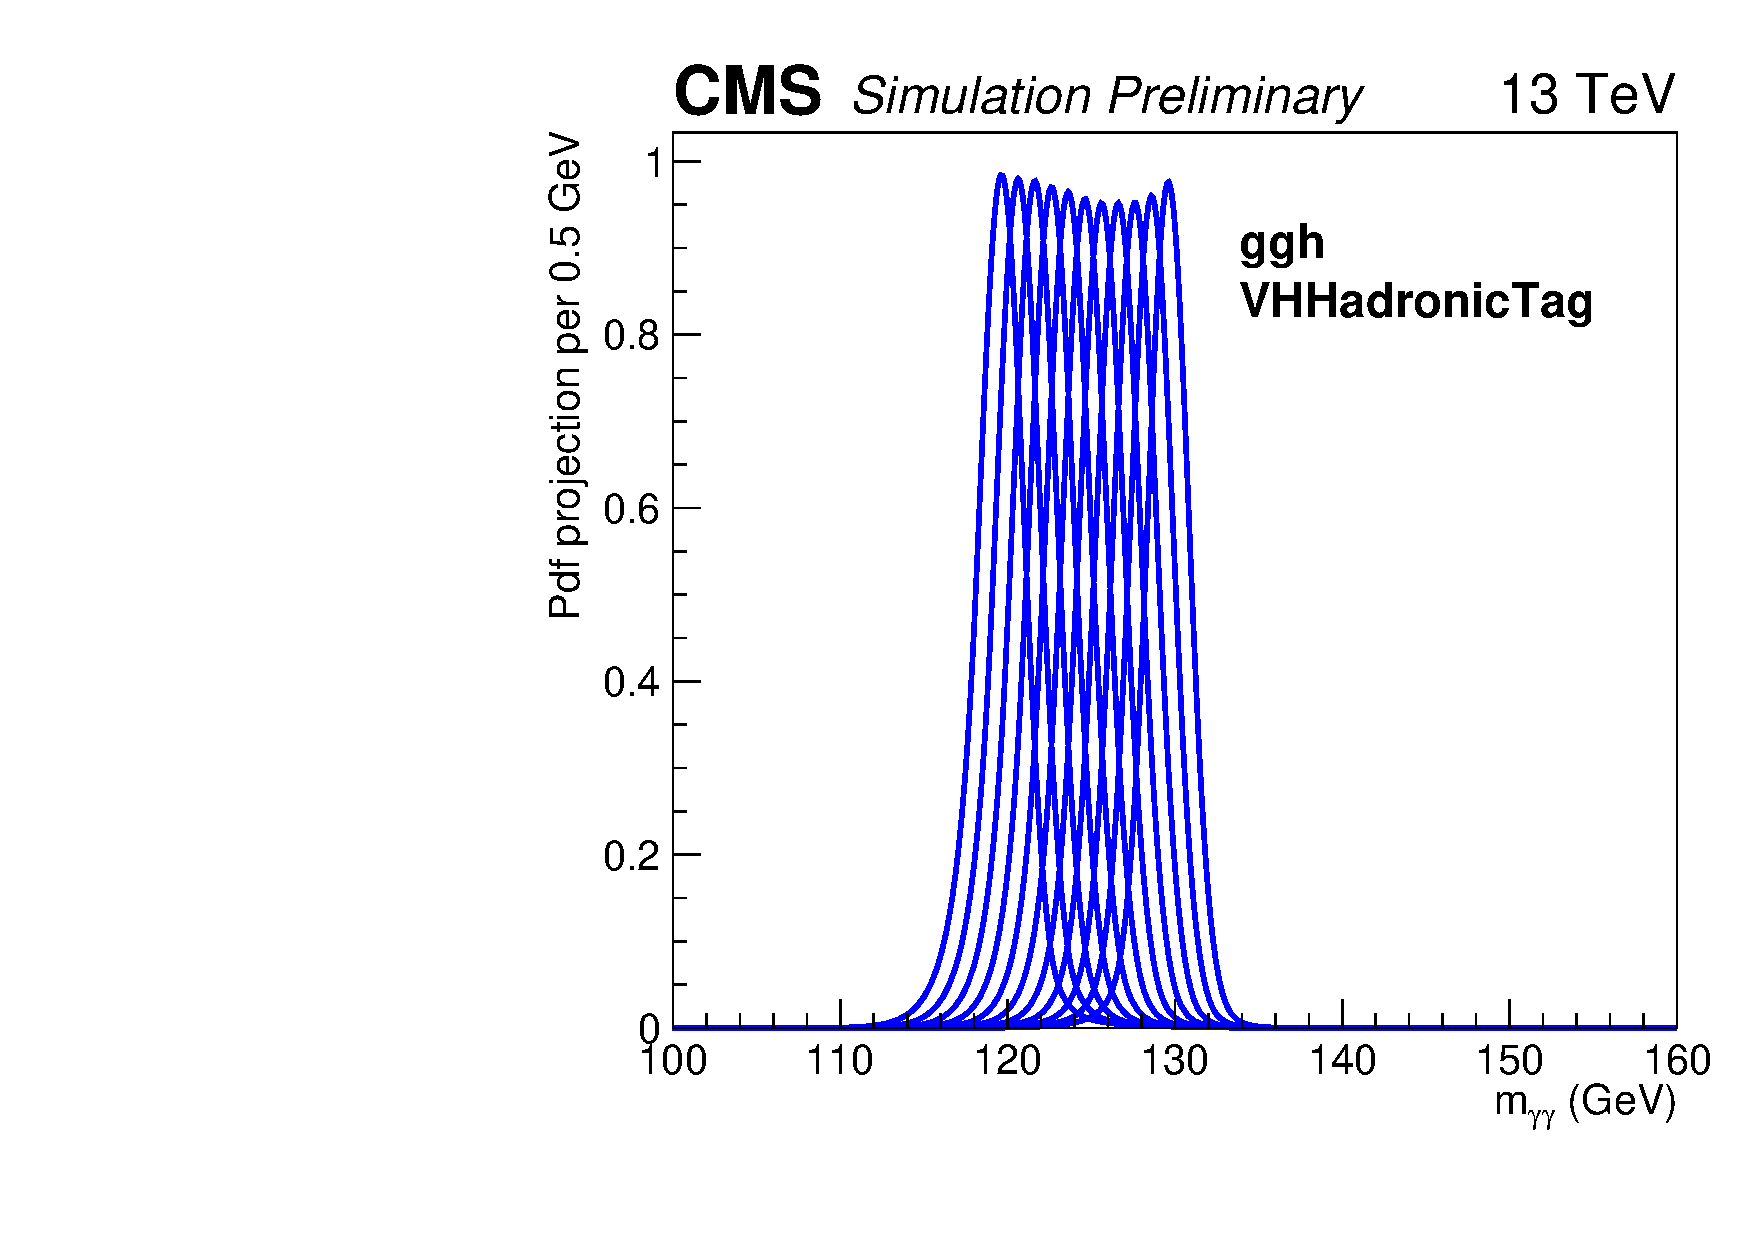
\includegraphics[width=0.47\textwidth]{modellingFigures/\whichFig/DCBpG/SSF/ggh_VHHadronicTag_fmc_interp.pdf}
%\caption{The \mH-dependence of the signal models for the ggH process for each of \VHTag categories is shown. Each curve shows the signal model for a given value of \mH. The contributions from the RV and WV components of each model were summed together according to their relative size, and interpolated between the samples for different \mH using the SSF method.}
%
%\label{fig:model:sig_interpolation_tris}
%\end{figure}
%\fi

\ifNewAnalysis
%The dependence of the full normalised parametric signal model on \mH for the \ggH process in each of the analysis categories is shown in \Fig\s~\ref{fig:model:sig_interpolation}, ~\ref{fig:model:sig_interpolation_bis} and~\ref{fig:model:sig_interpolation_tris}.
The normalised signal models for each process and category, evaluated at $\mH=125\GeV$ after parametrising all mass points with the \DCBpG and interpolating using \SSF, are available in \App~\ref{app:modelling} in \Fig\s~\ref{fig:model:sig_model_per_ggh}, ~\ref{fig:model:sig_model_per_vbf}, ~\ref{fig:model:sig_model_per_tth}, ~\ref{fig:model:sig_model_per_wh}, and~\ref{fig:model:sig_model_per_zh}.
The normalised signal models for each process are summed together to obtain the expected signal \mgg distribution for all categories combined (as shown in \Fig\s~\ref{fig:model:sig_model_all}), or for individual analysis categories (as shown in \Fig\s~\ref{fig:model:sig_model_per_category},~\ref{fig:model:sig_model_per_category_bis} and~\ref{fig:model:sig_model_per_category_tris}).
\else
%The dependence of the full normalised parametric signal model on \mH for the \ggH process in each of the analysis categories is shown in \Fig\s~\ref{fig:model:sig_interpolation} and~\ref{fig:model:sig_interpolation_bis}.
The normalised signal models for each process are summed together to obtain the expected signal \mgg distribution for all categories combined (as shown in \Fig\s~\ref{fig:model:sig_model_all}), or for individual analysis categories (as shown in \Fig\s~\ref{fig:model:sig_model_per_category} and~\ref{fig:model:sig_model_per_category_bis}).
\fi
\begin{figure}[ht!]
\centering
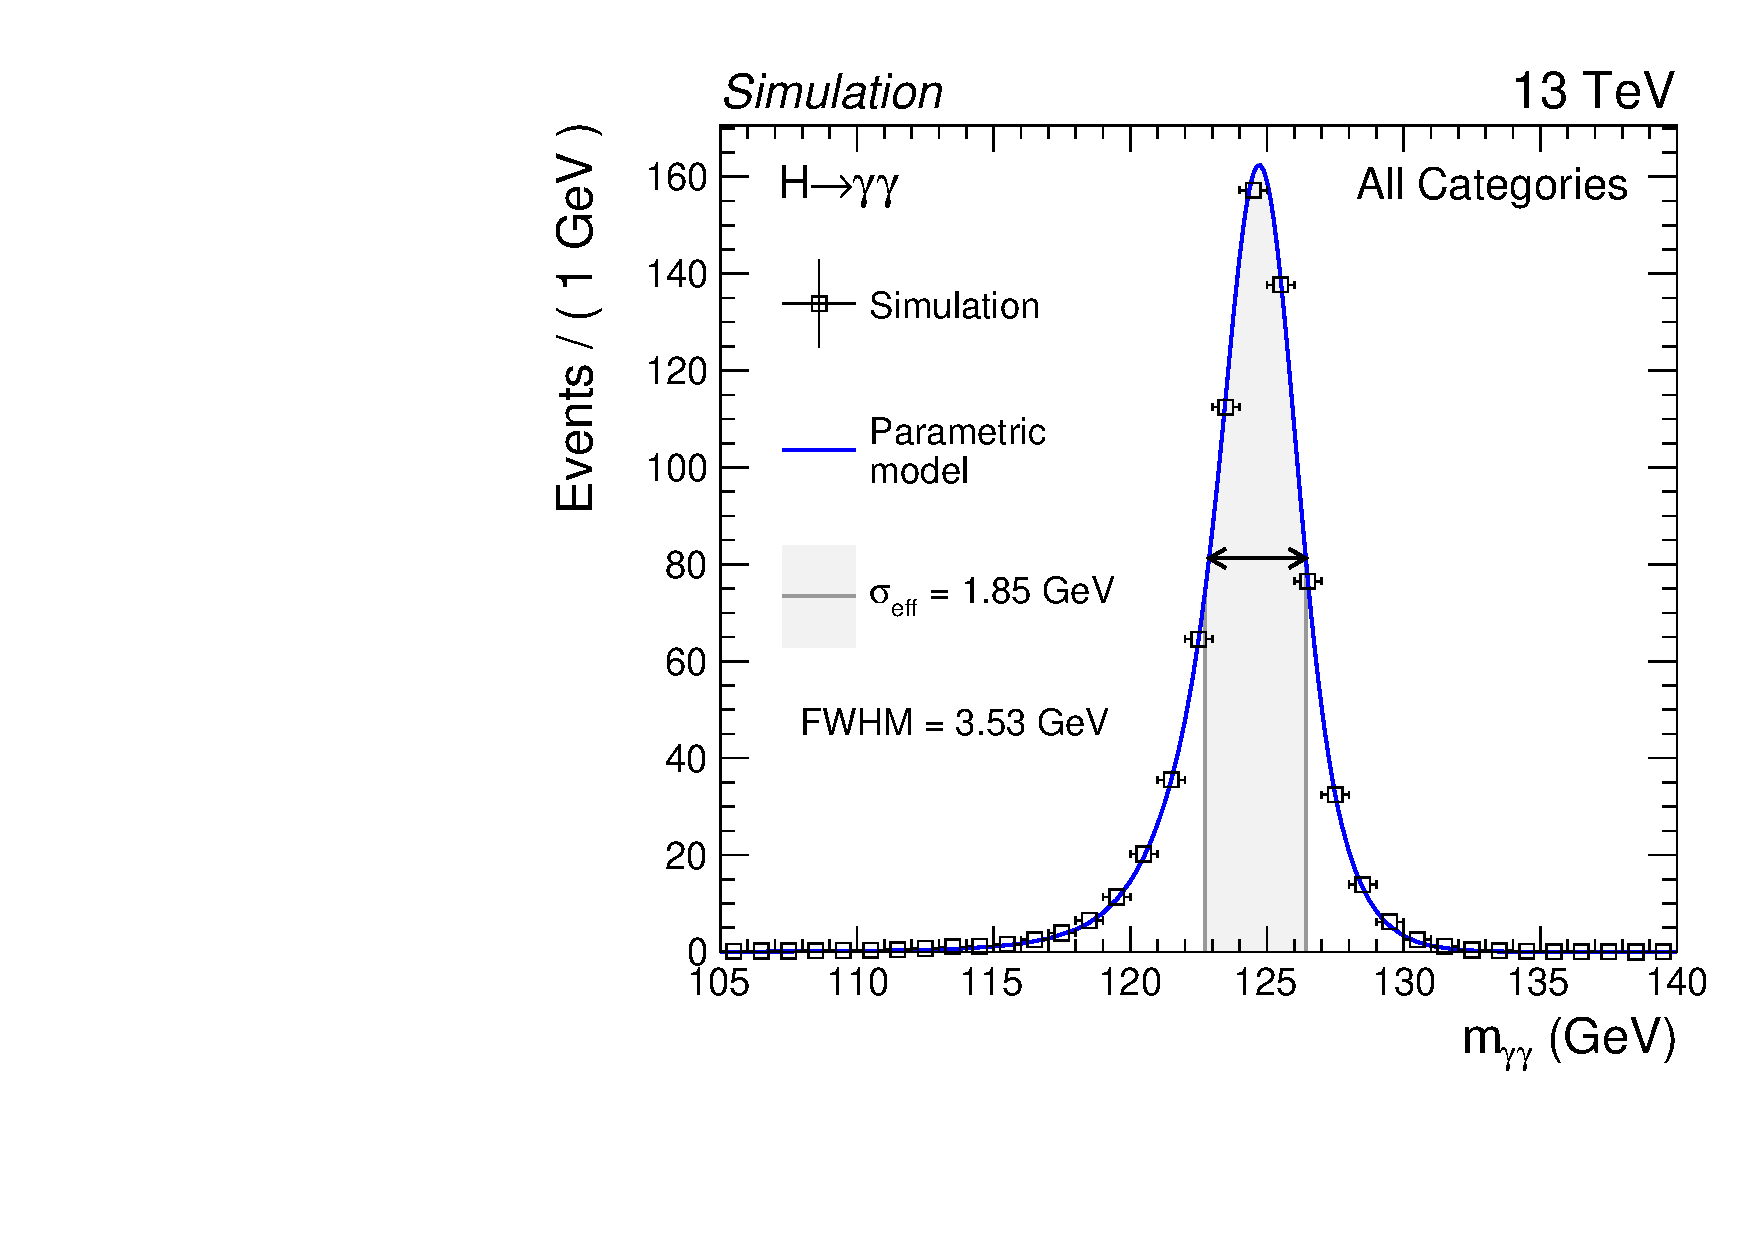
\includegraphics[width=0.75\textwidth]{modellingFigures/\whichFig/DCBpG/SSF/all.pdf} 

\caption{The signal model for all analysis categories combined for $\mH=125\GeV$, obtained by summing the contributions from each production process according to the \effxacc. The \effSigma (half the width of the narrowest interval containing 68.3\% of the invariant mass distribution) and the FWHM (the width of the distribution at half of the maximum value) are also shown. }

\label{fig:model:sig_model_all}
\end{figure}

\begin{figure}[htp!]
\centering
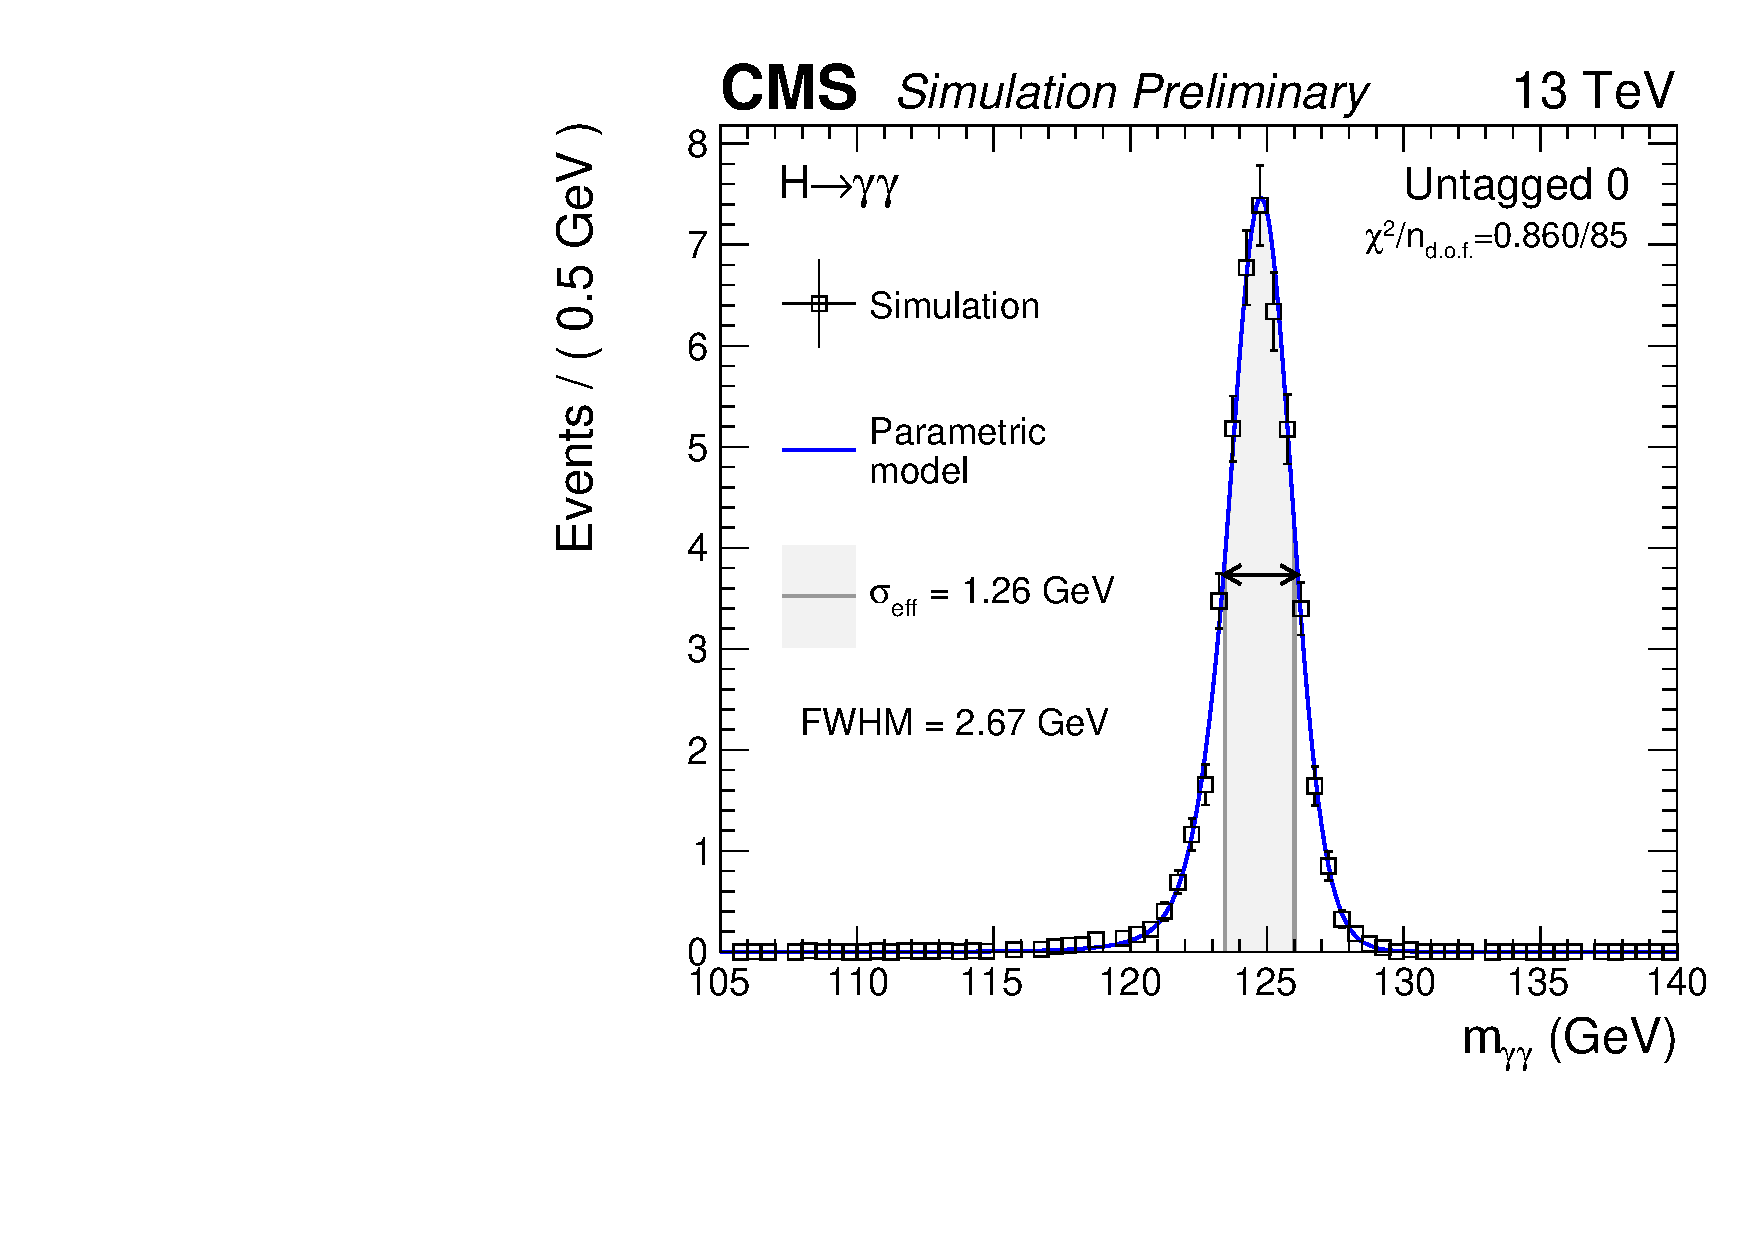
\includegraphics[width=0.45\textwidth]{modellingFigures/\whichFig/DCBpG/SSF/UntaggedTag_0.pdf} 
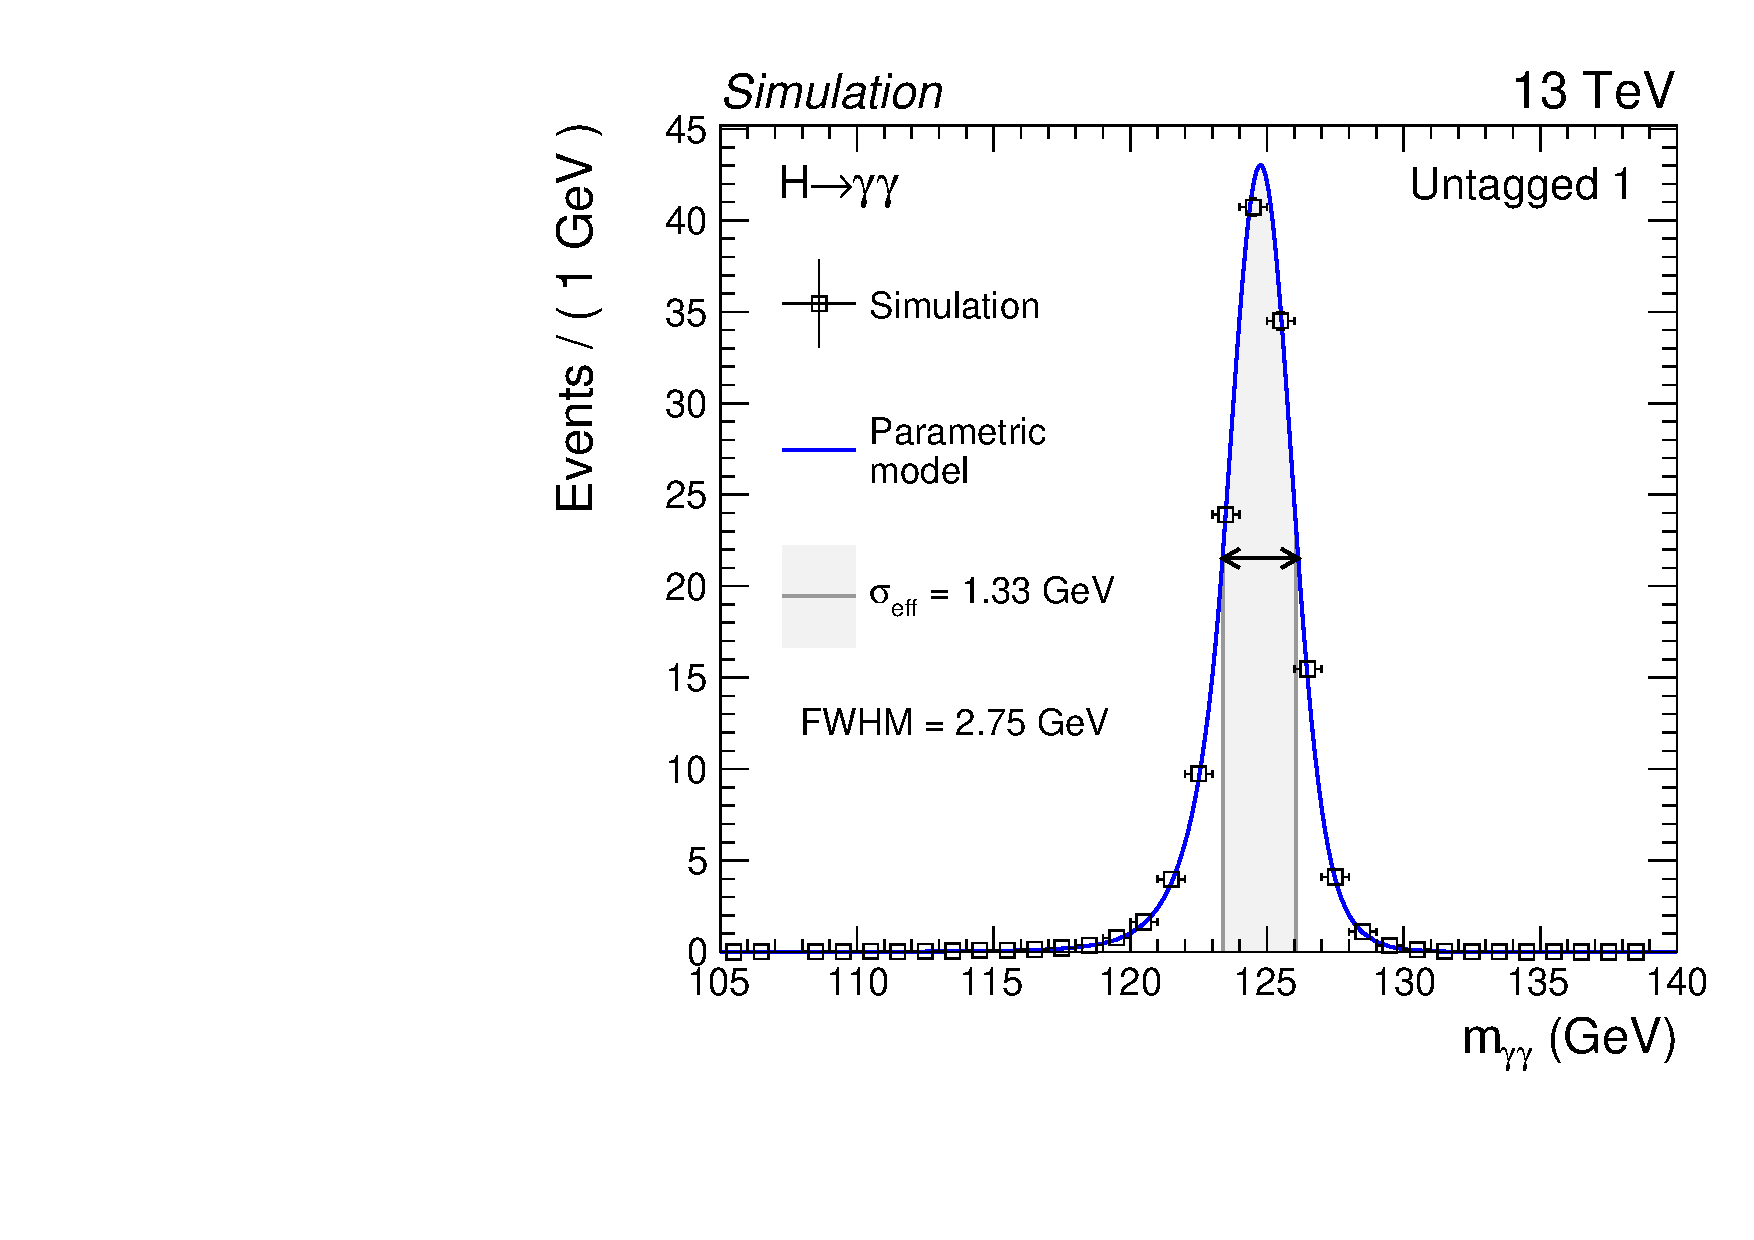
\includegraphics[width=0.45\textwidth]{modellingFigures/\whichFig/DCBpG/SSF/UntaggedTag_1.pdf} \\
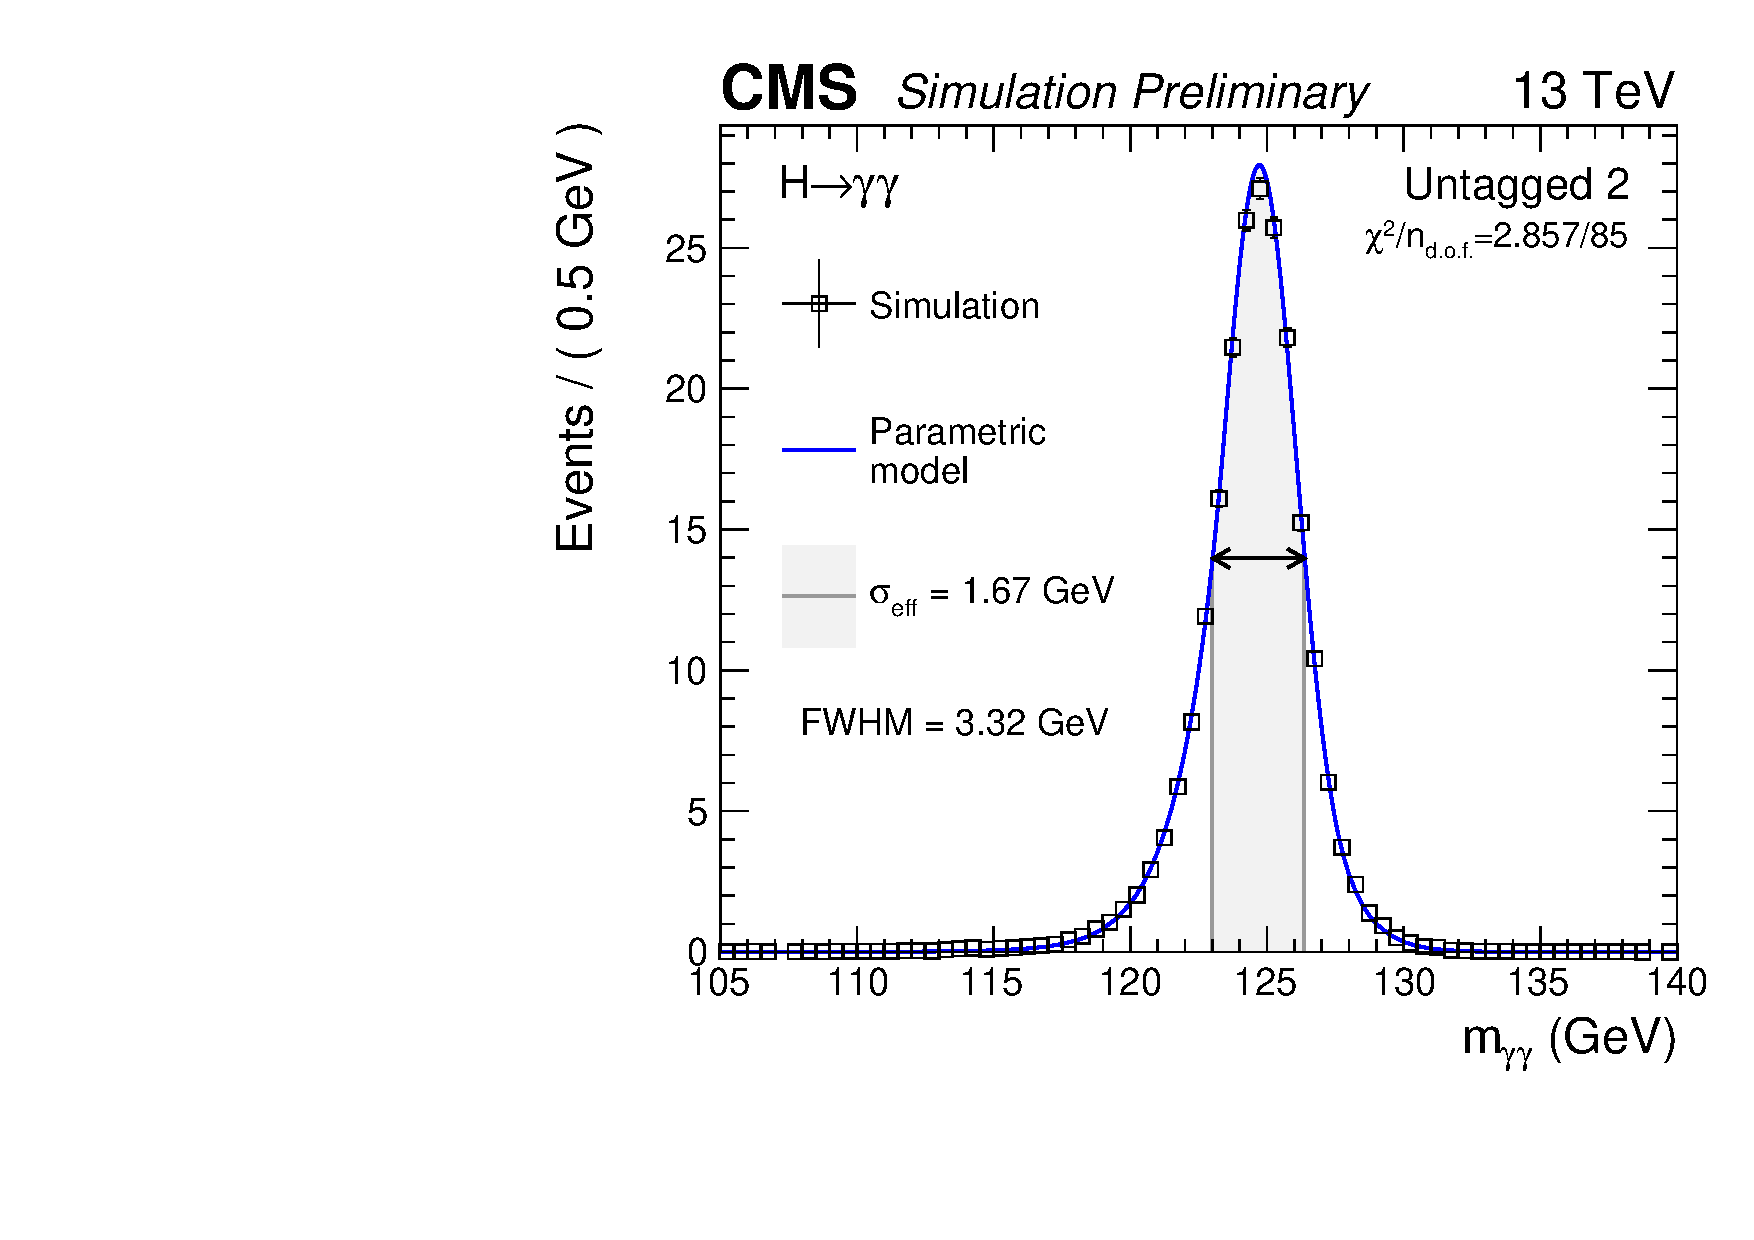
\includegraphics[width=0.45\textwidth]{modellingFigures/\whichFig/DCBpG/SSF/UntaggedTag_2.pdf} 
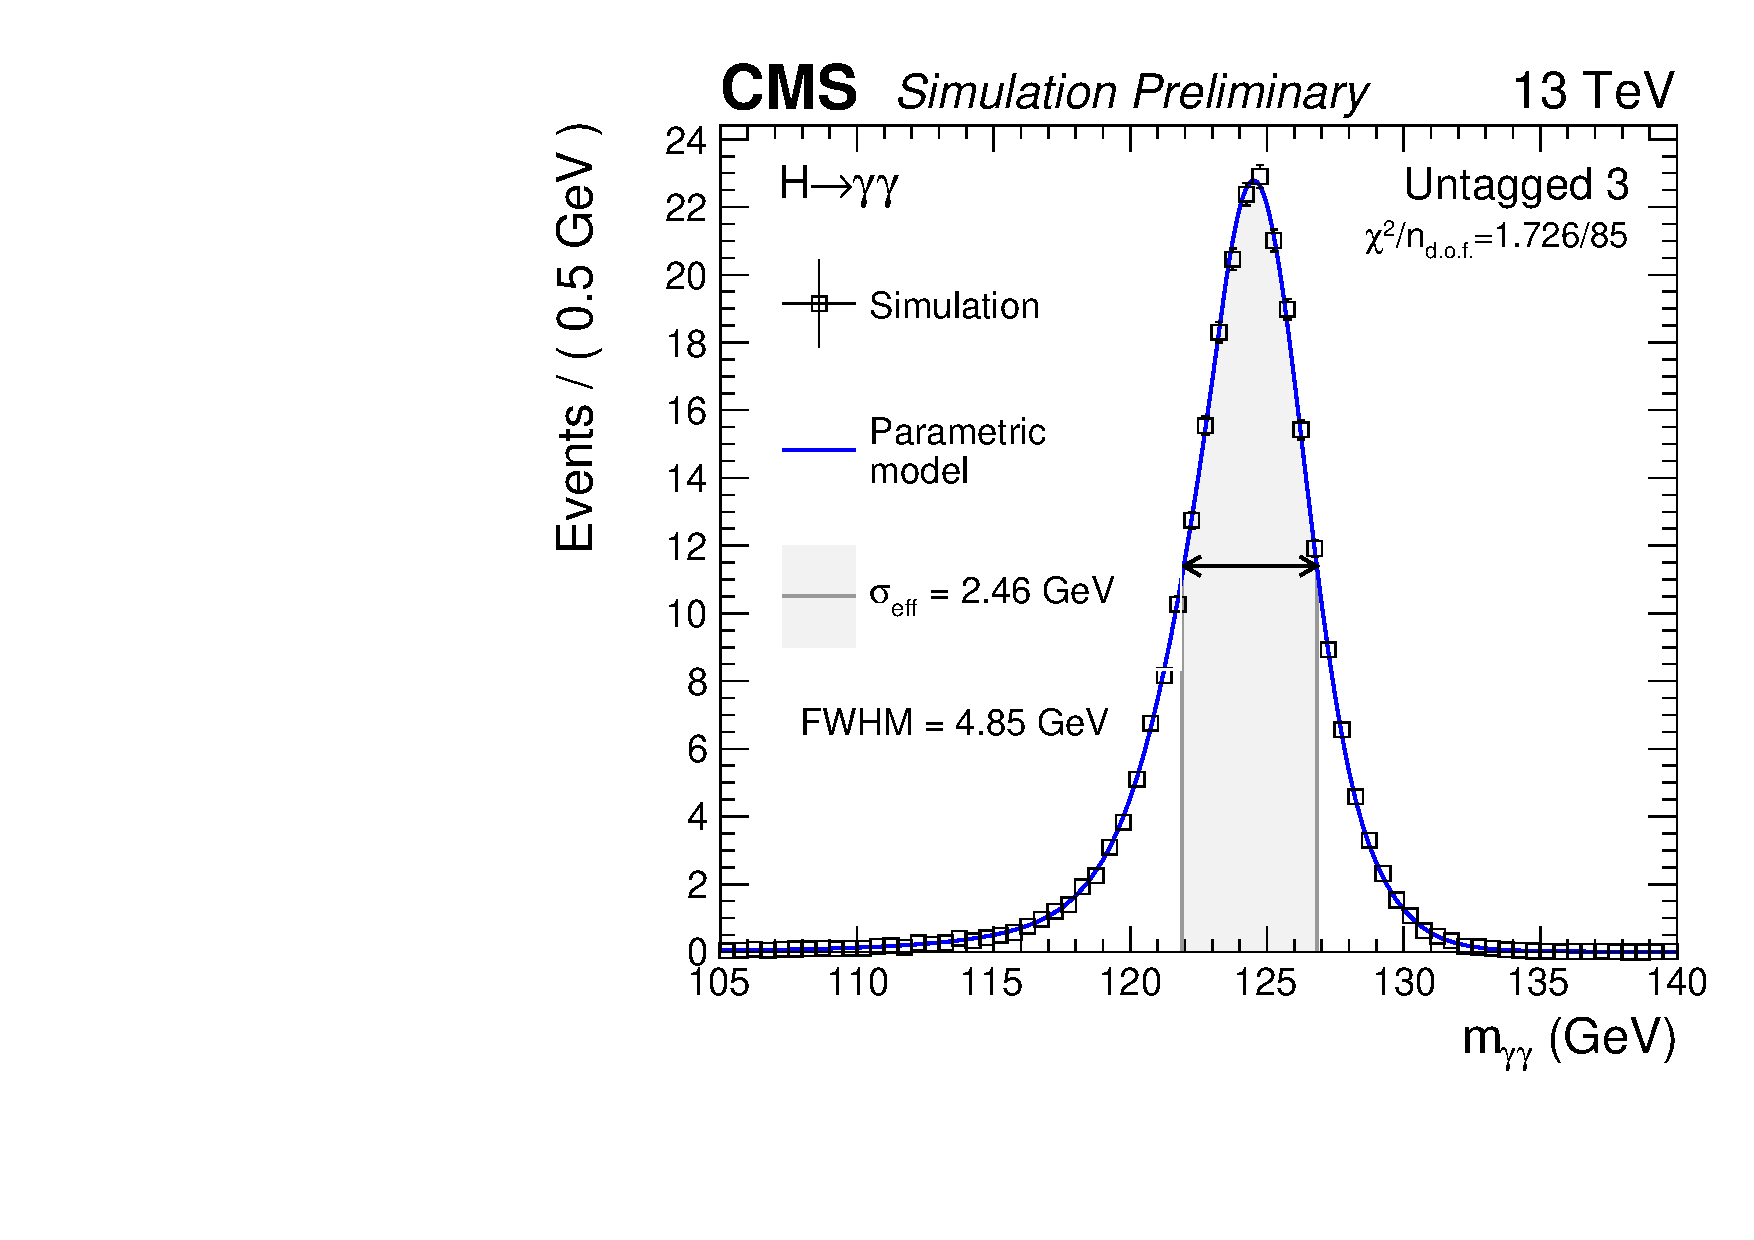
\includegraphics[width=0.45\textwidth]{modellingFigures/\whichFig/DCBpG/SSF/UntaggedTag_3.pdf} \\ 

\caption{The signal models for the \Untagged analysis categories for $\mH=125\GeV$, obtained by summing the contributions from each production process according to their \effxacc. The \effSigma (half the width of the narrowest interval containing 68.3\% of the invariant mass distribution) and the FWHM (the width of the distribution at half of the maximum value) are also shown.}

\label{fig:model:sig_model_per_category}
\end{figure}

\begin{figure}[htp!]
\centering
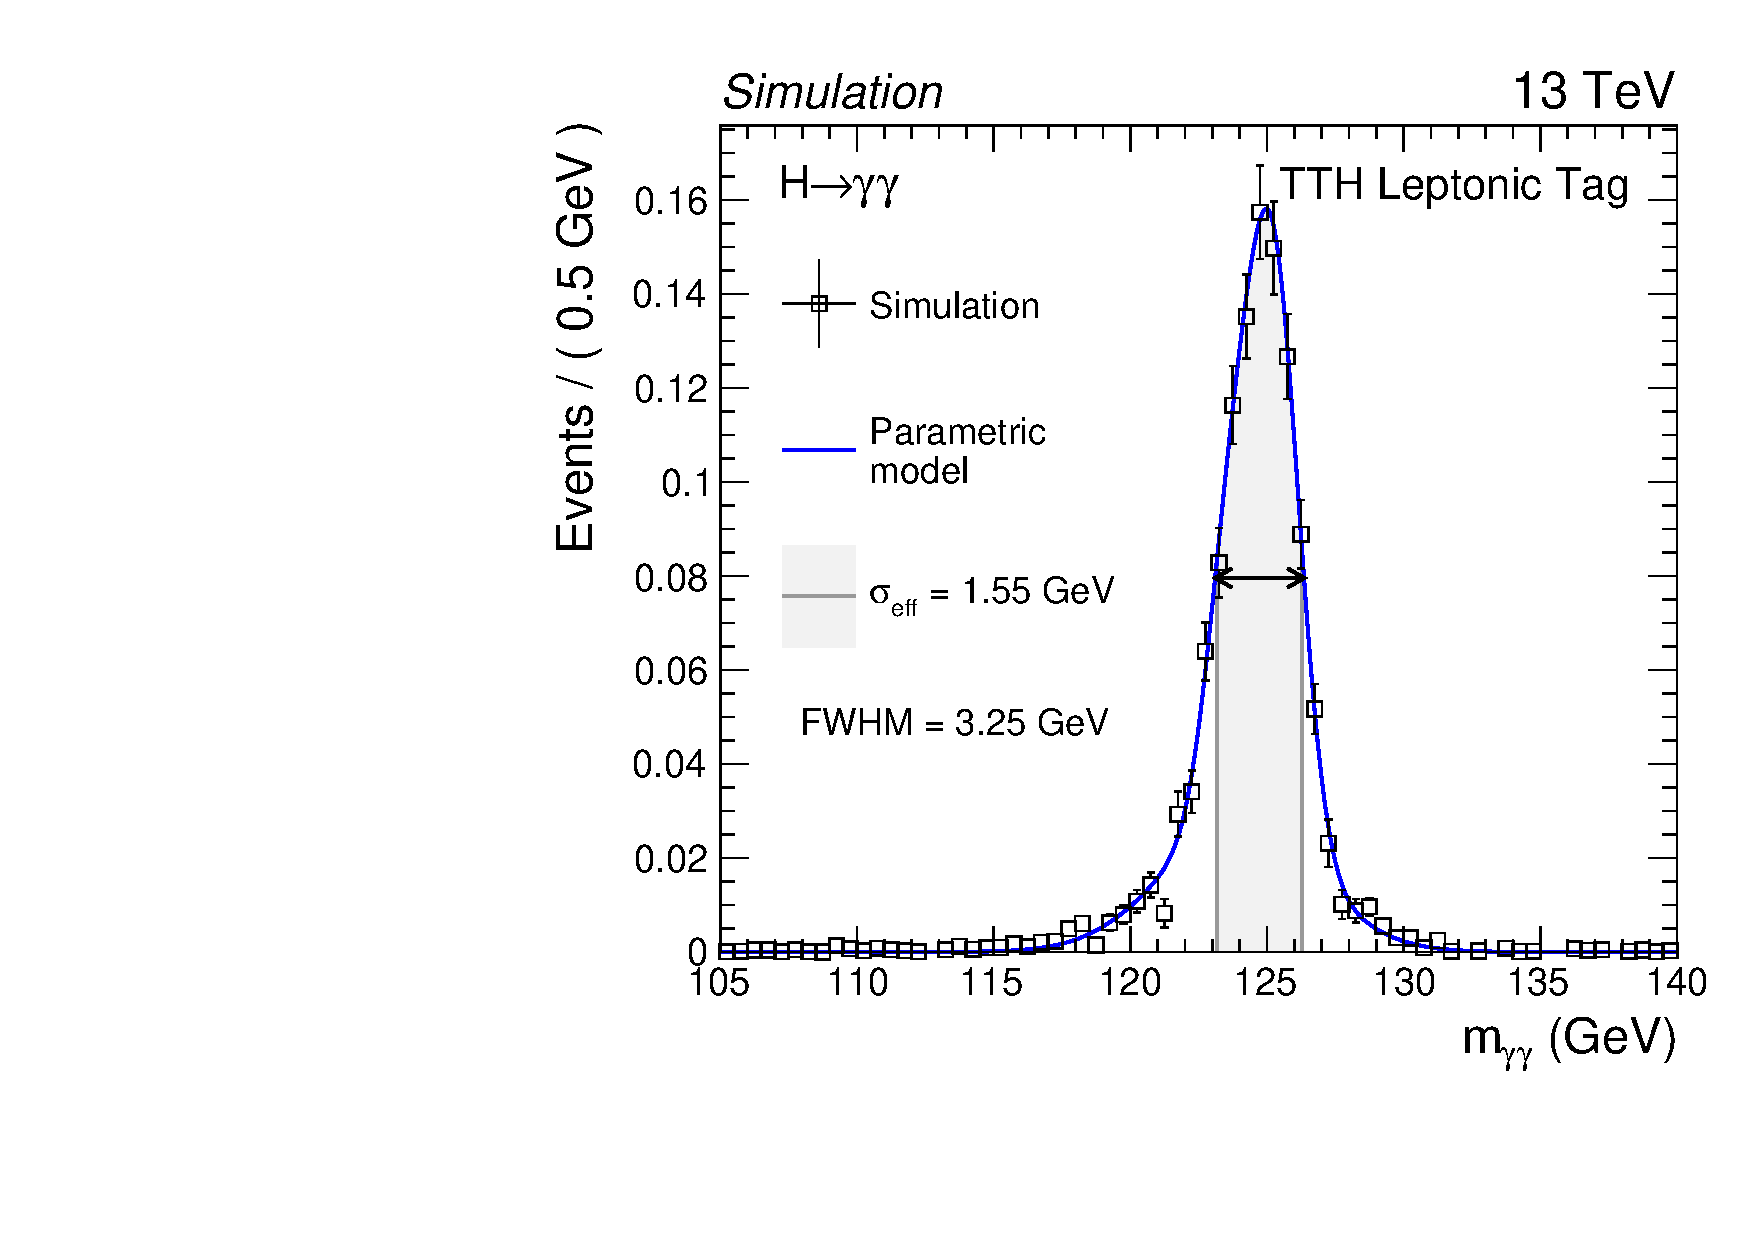
\includegraphics[width=0.45\textwidth]{modellingFigures/\whichFig/DCBpG/SSF/TTHLeptonicTag.pdf} 
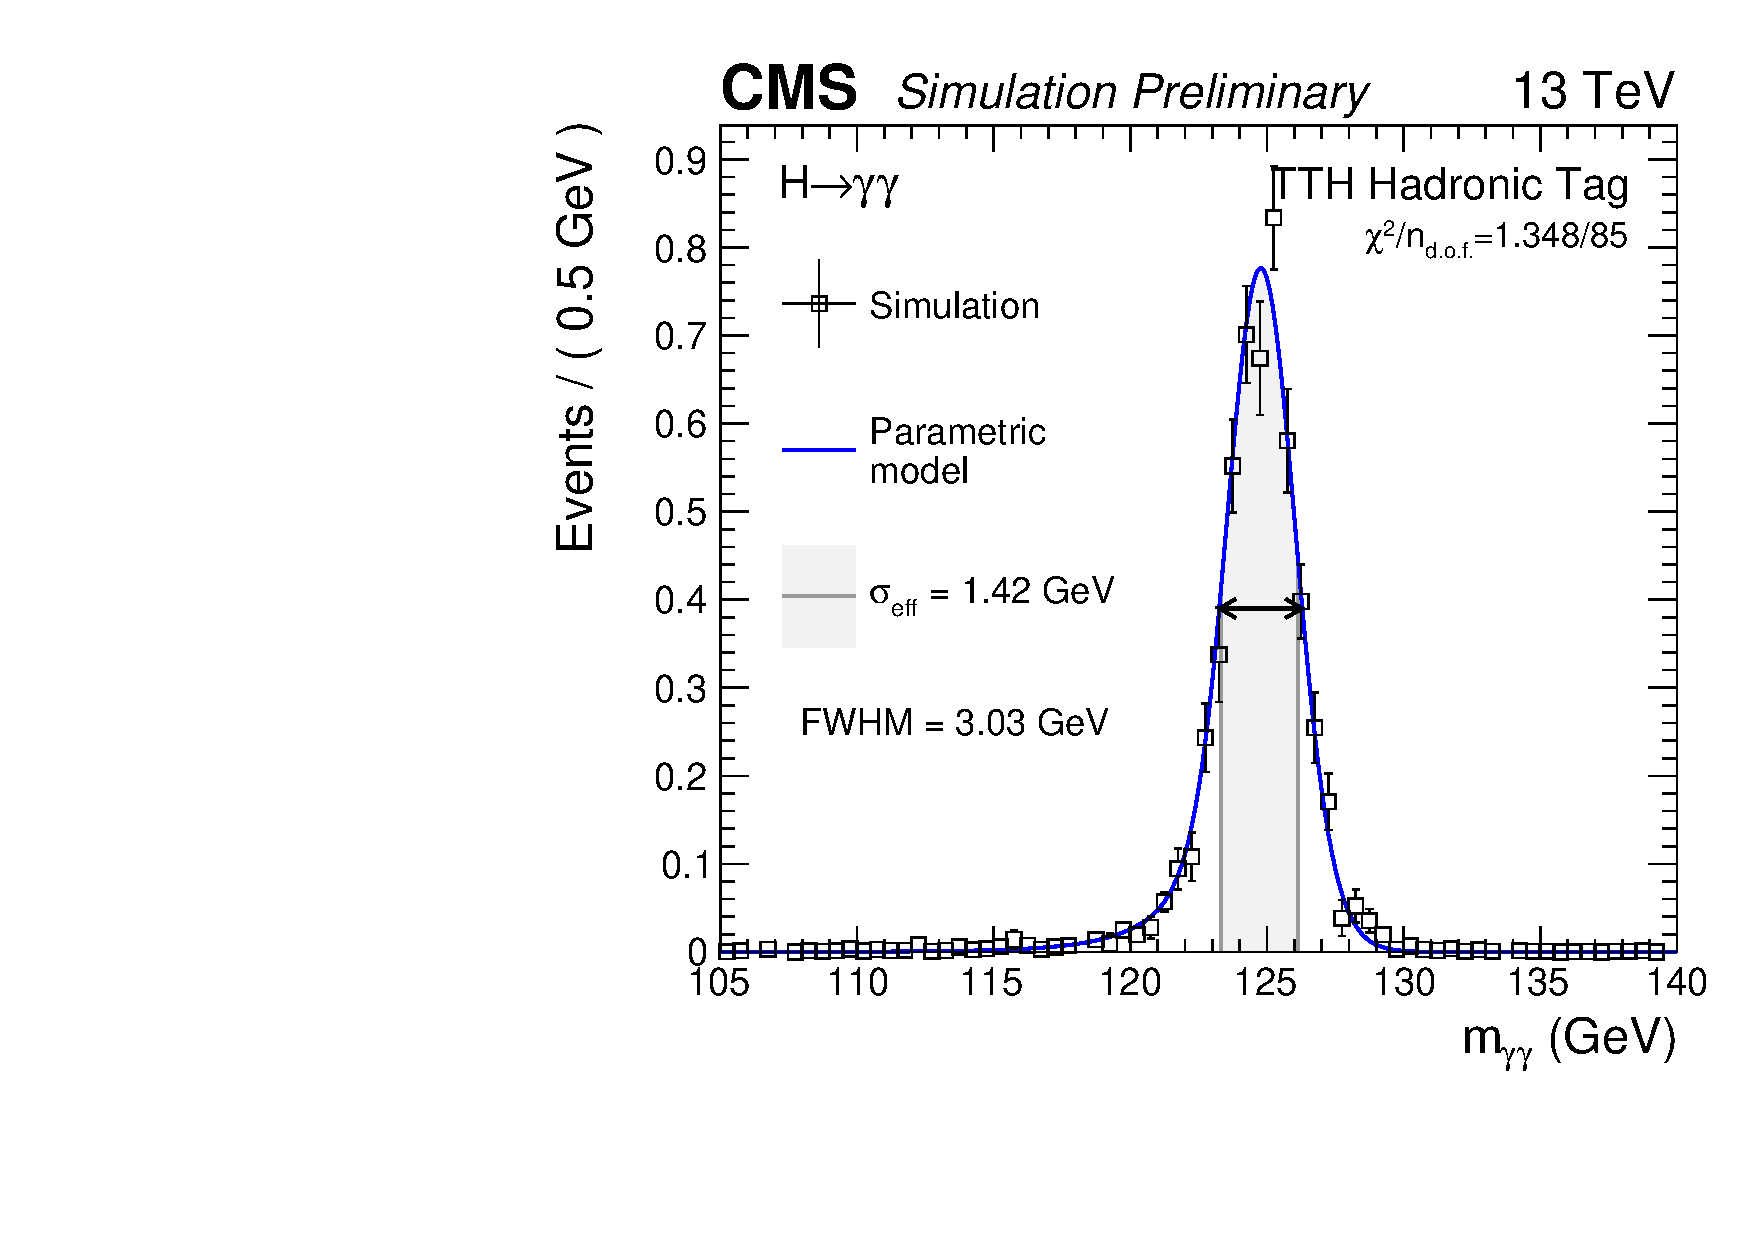
\includegraphics[width=0.45\textwidth]{modellingFigures/\whichFig/DCBpG/SSF/TTHHadronicTag.pdf} \\
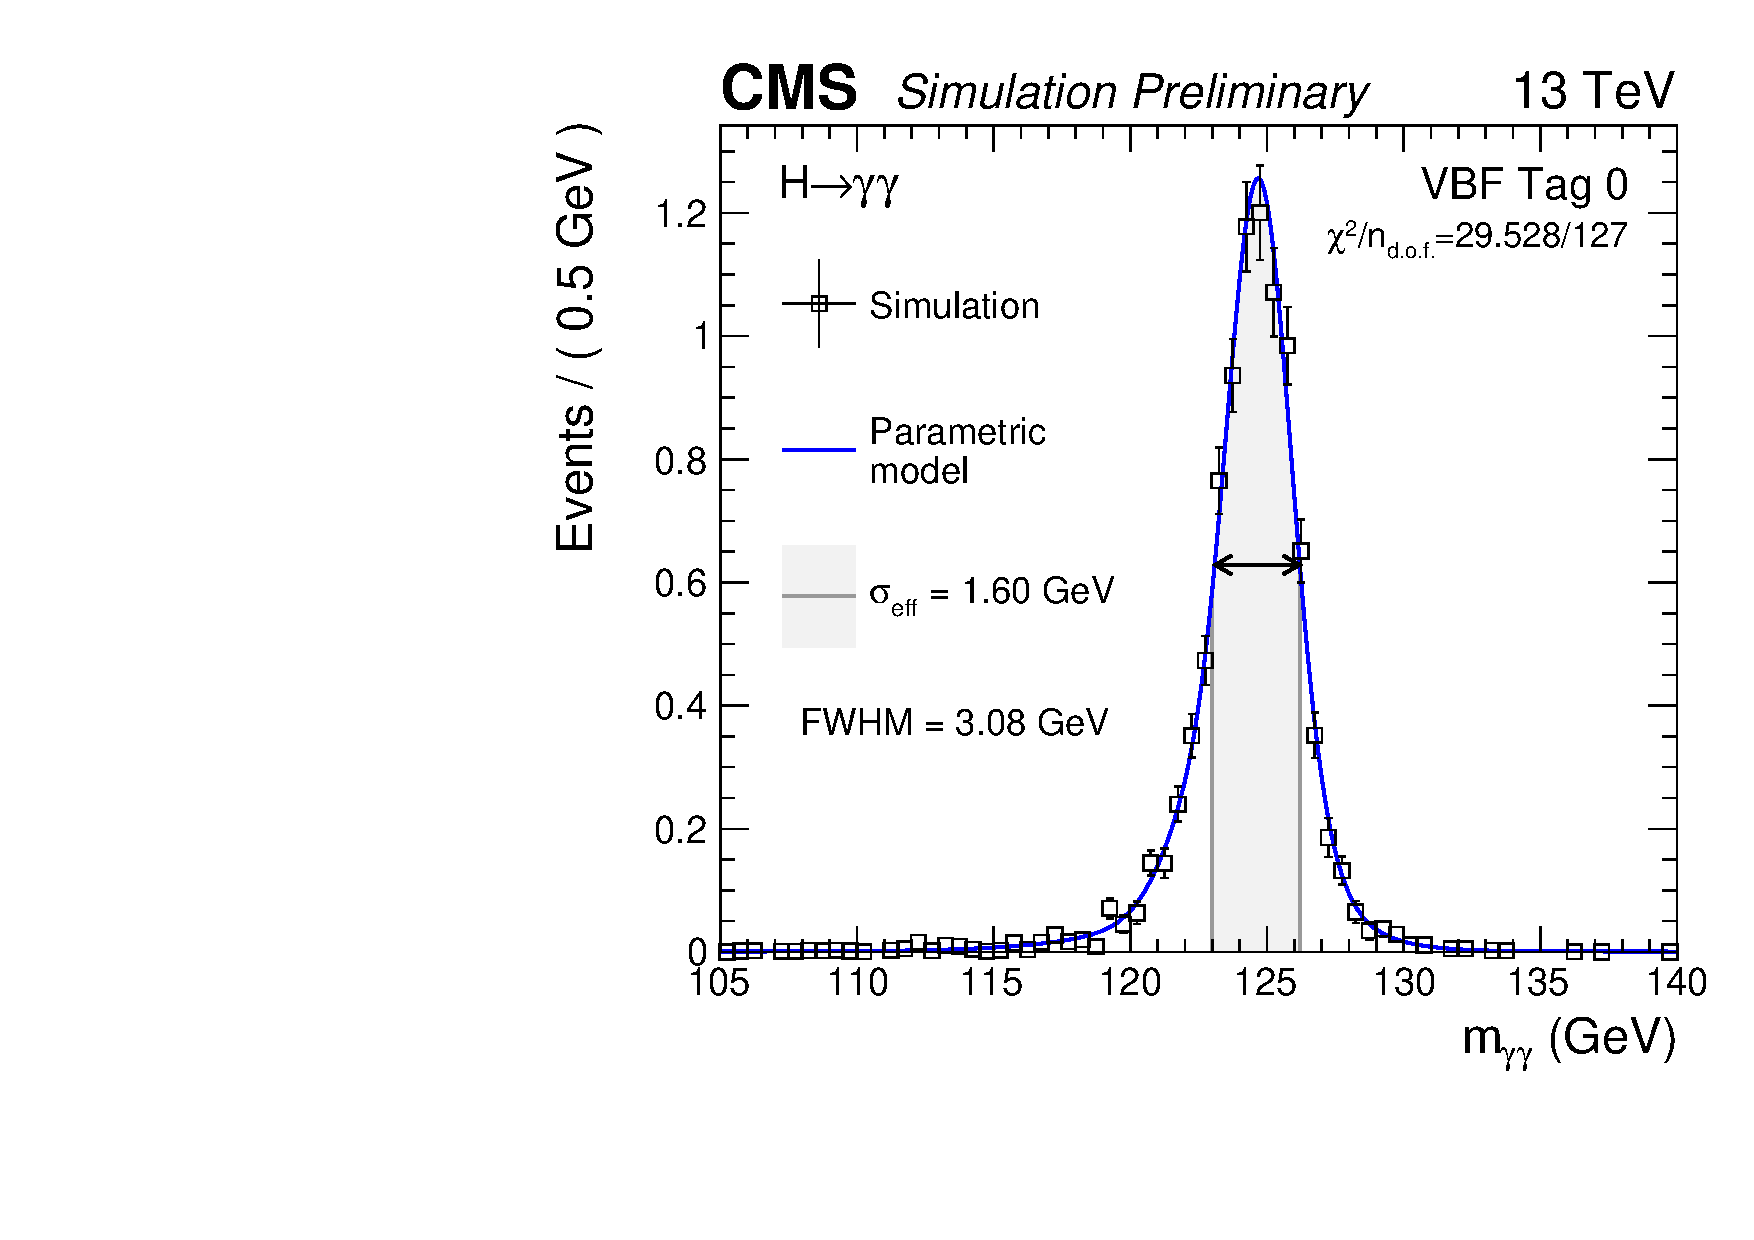
\includegraphics[width=0.45\textwidth]{modellingFigures/\whichFig/DCBpG/SSF/VBFTag_0.pdf} 
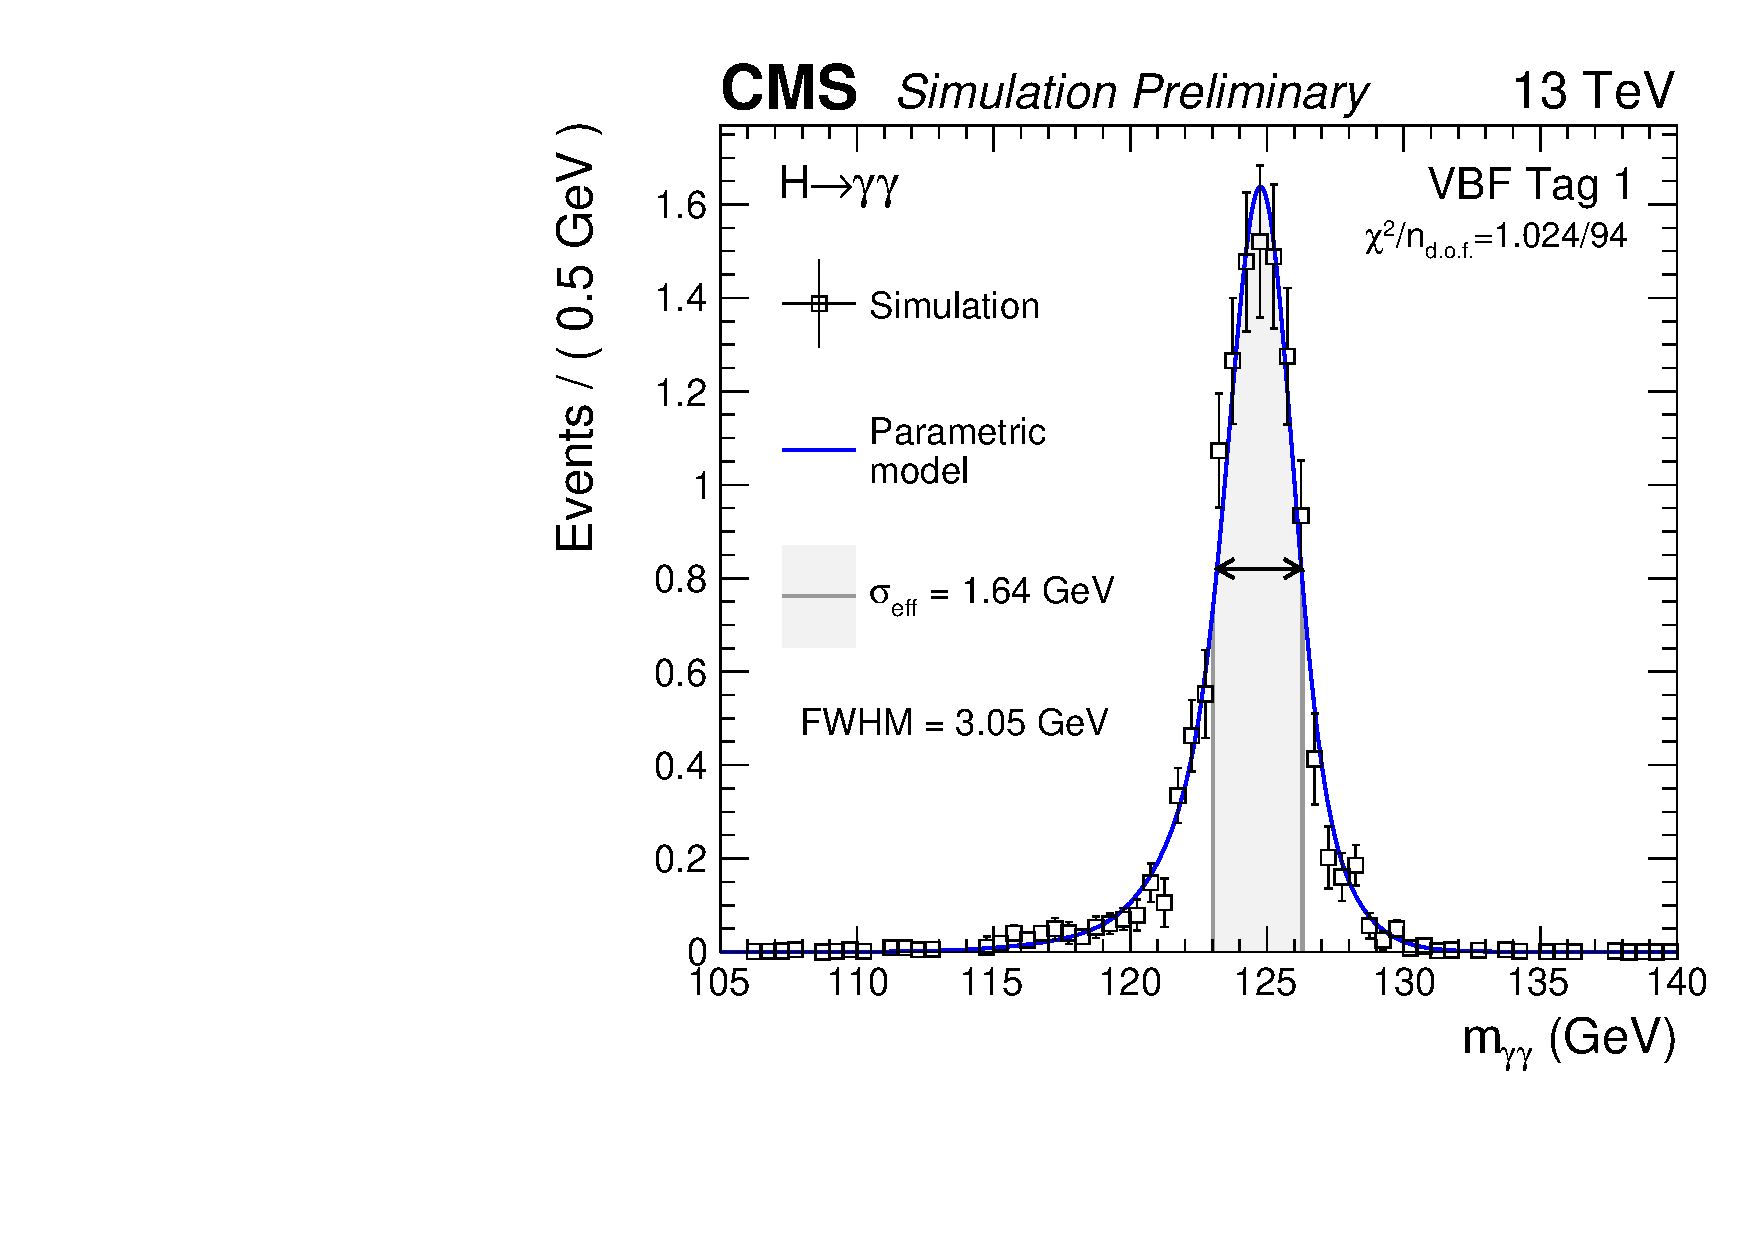
\includegraphics[width=0.45\textwidth]{modellingFigures/\whichFig/DCBpG/SSF/VBFTag_1.pdf}\\ 
\ifNewAnalysis
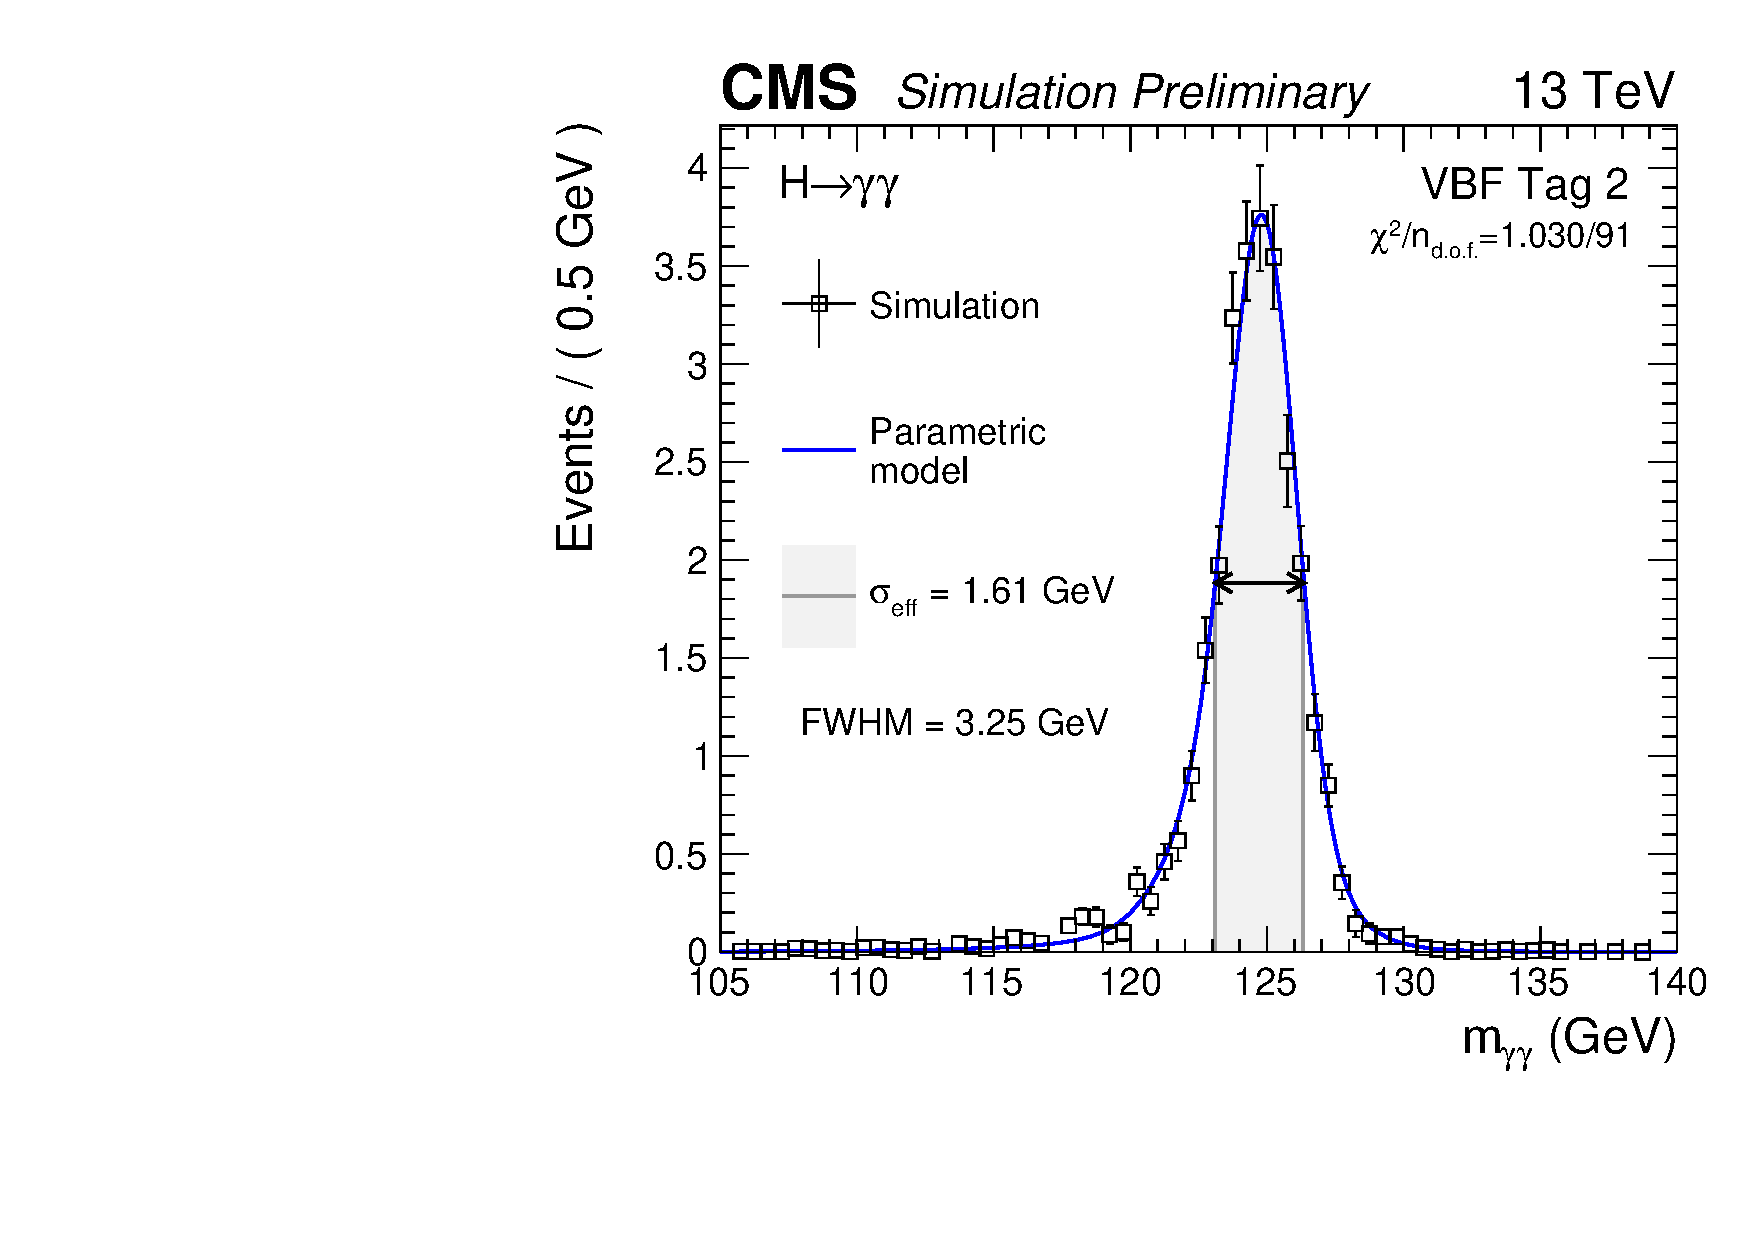
\includegraphics[width=0.45\textwidth]{modellingFigures/\whichFig/DCBpG/SSF/VBFTag_2.pdf} 
\fi
\caption{The signal models for the \VBFTag and \TTHTag analysis categories for $\mH=125\GeV$, obtained by summing the contributions from each production process according to their \effxacc. The \effSigma (half the width of the narrowest interval containing 68.3\% of the invariant mass distribution) and the FWHM (the width of the distribution at half of the maximum value) are also shown.}

\label{fig:model:sig_model_per_category_bis}
\end{figure}

\ifNewAnalysis
\begin{figure}[htp!]
\centering
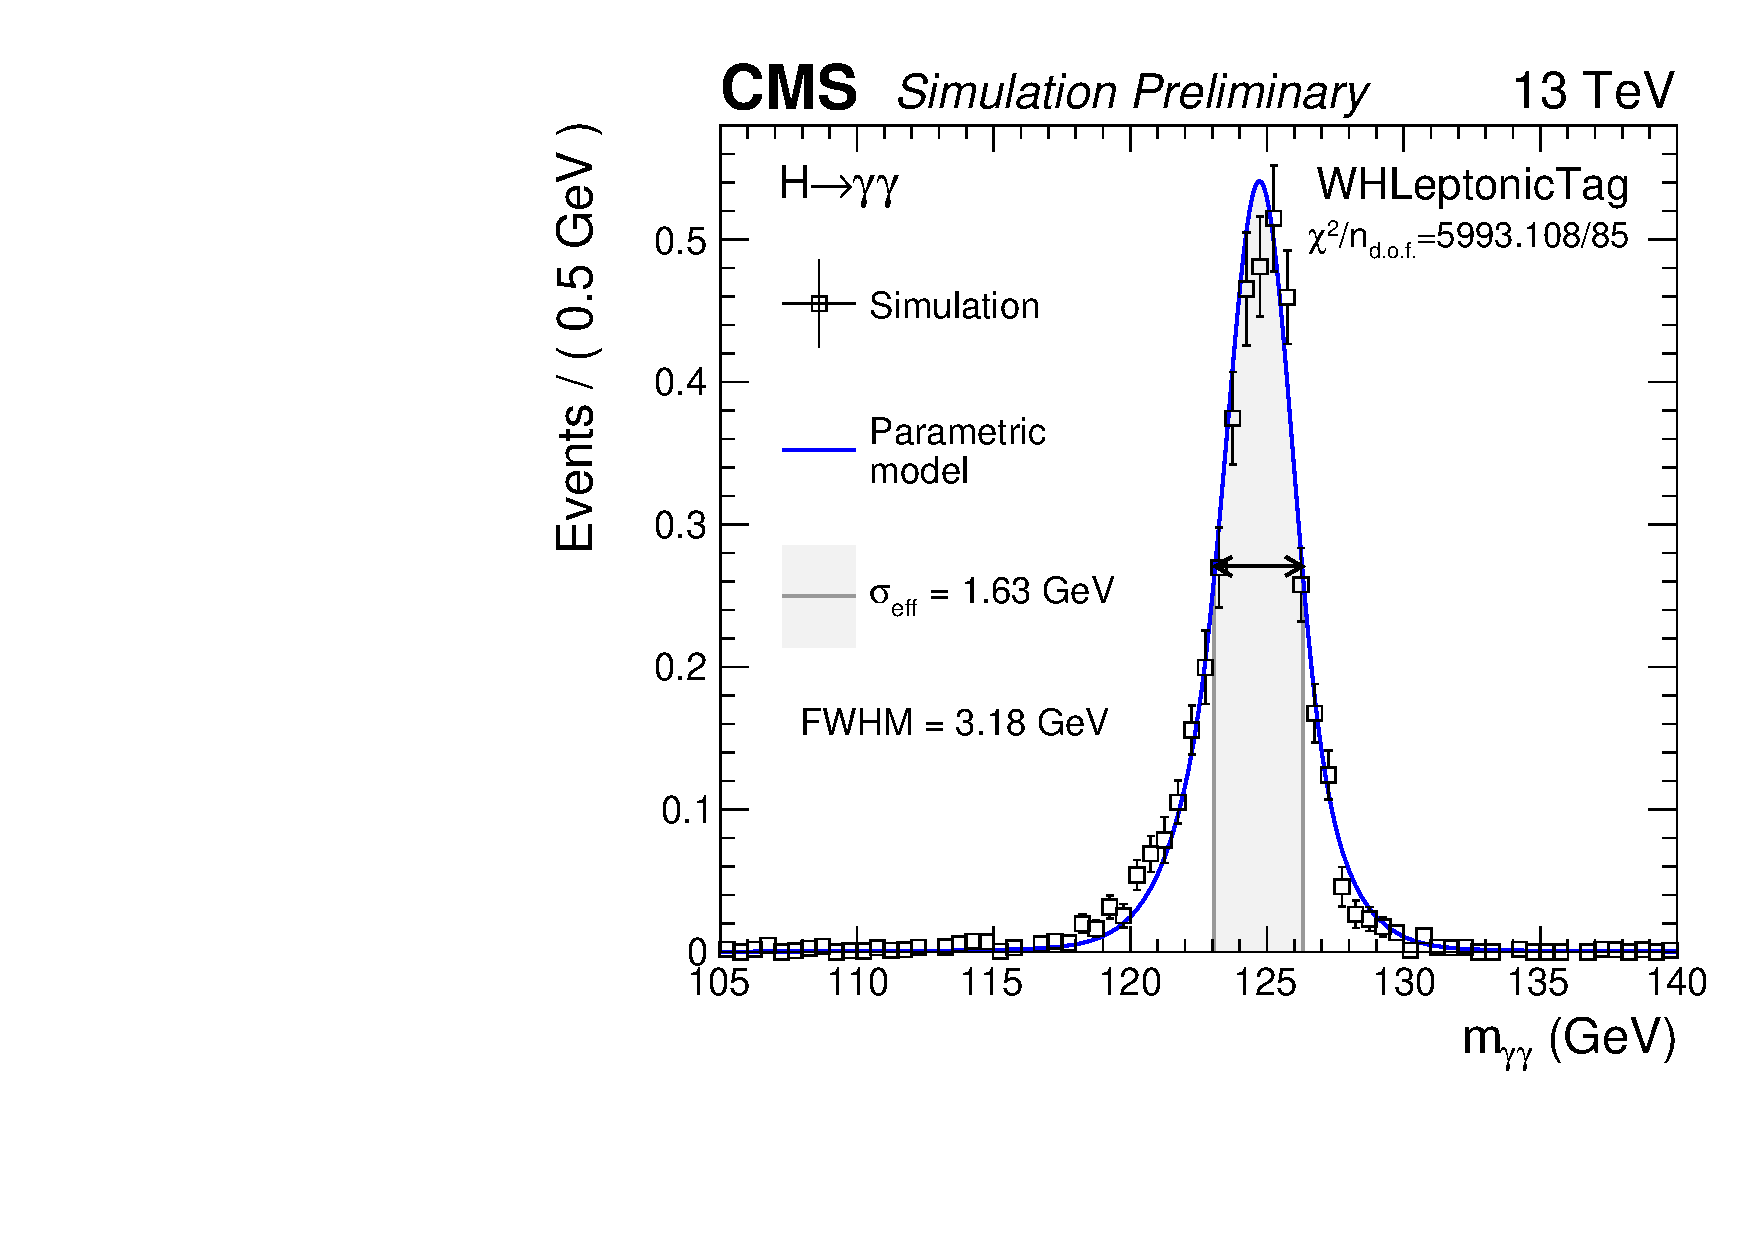
\includegraphics[width=0.45\textwidth]{modellingFigures/\whichFig/DCBpG/SSF/WHLeptonicTag.pdf} 
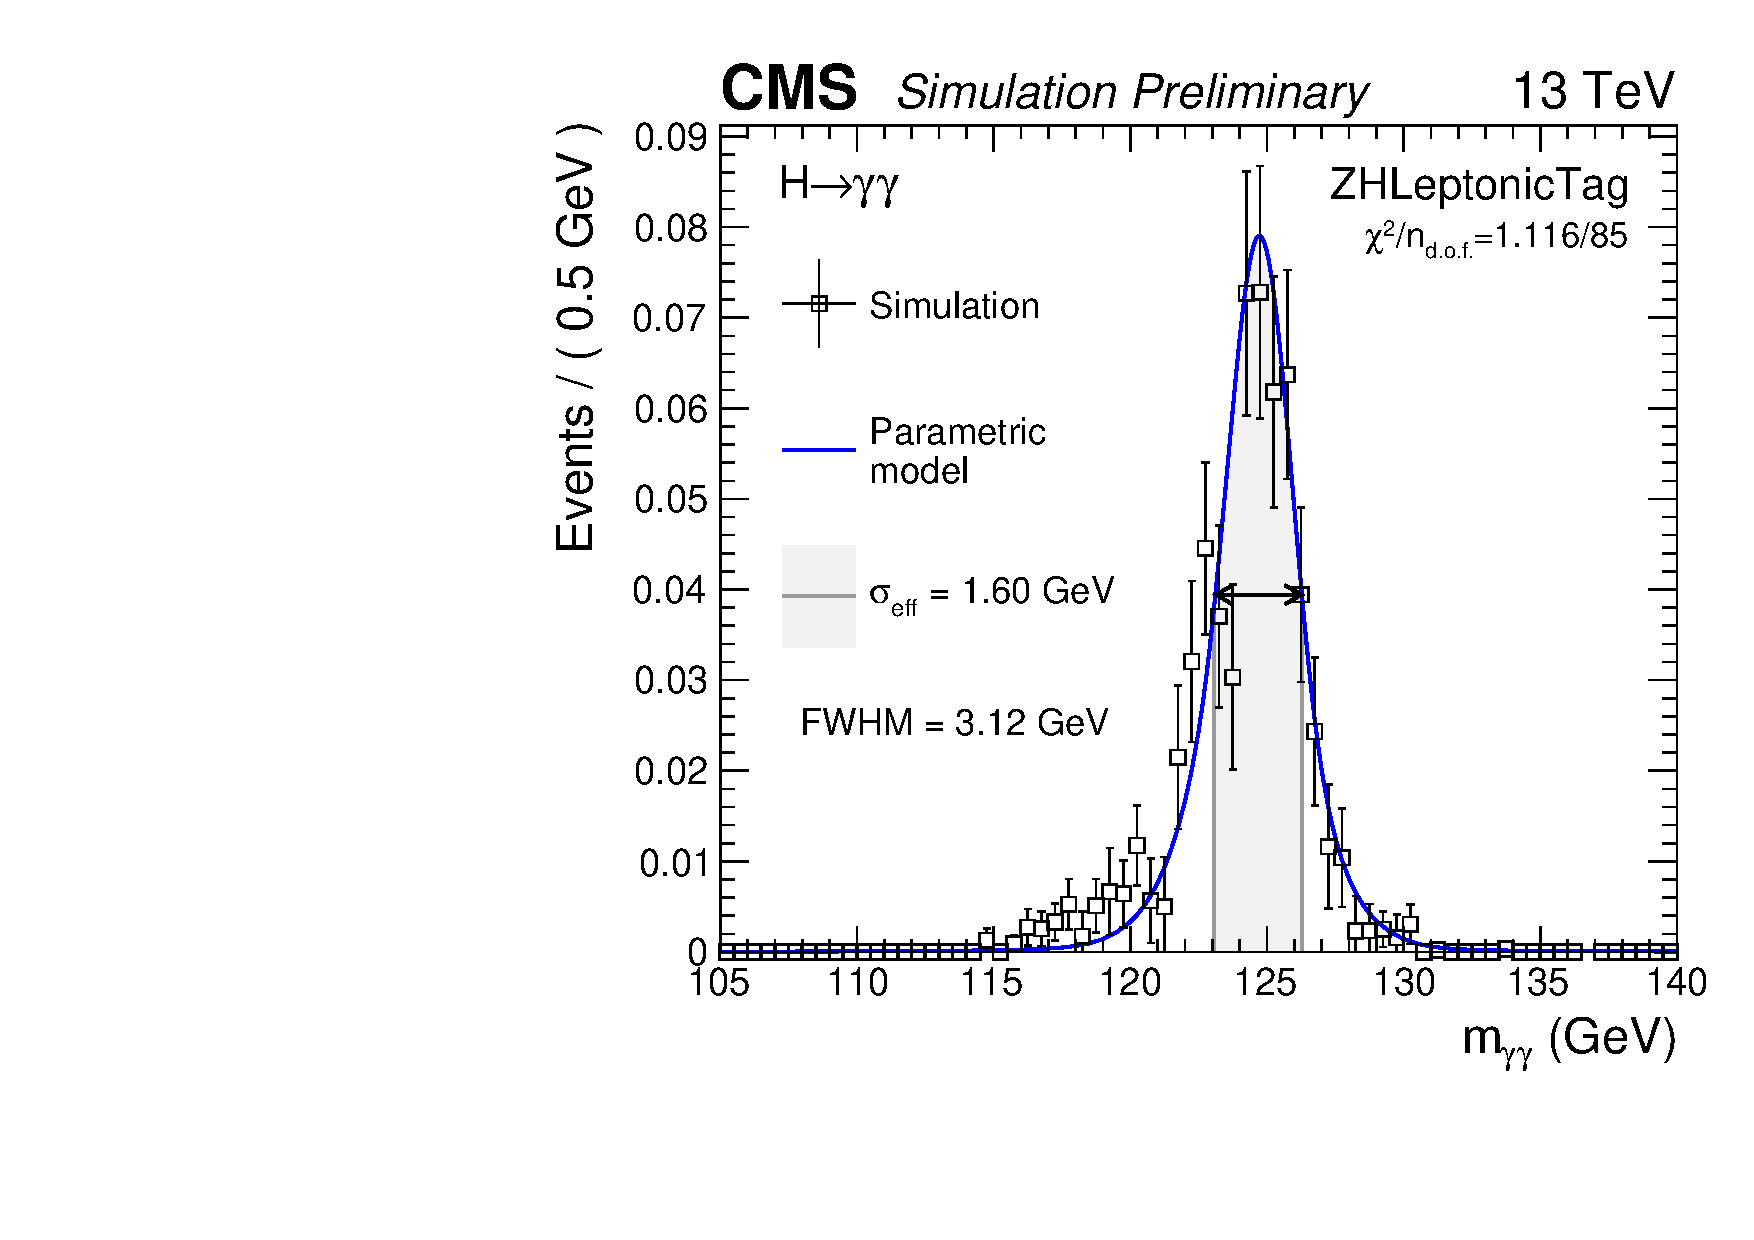
\includegraphics[width=0.45\textwidth]{modellingFigures/\whichFig/DCBpG/SSF/ZHLeptonicTag.pdf} \\
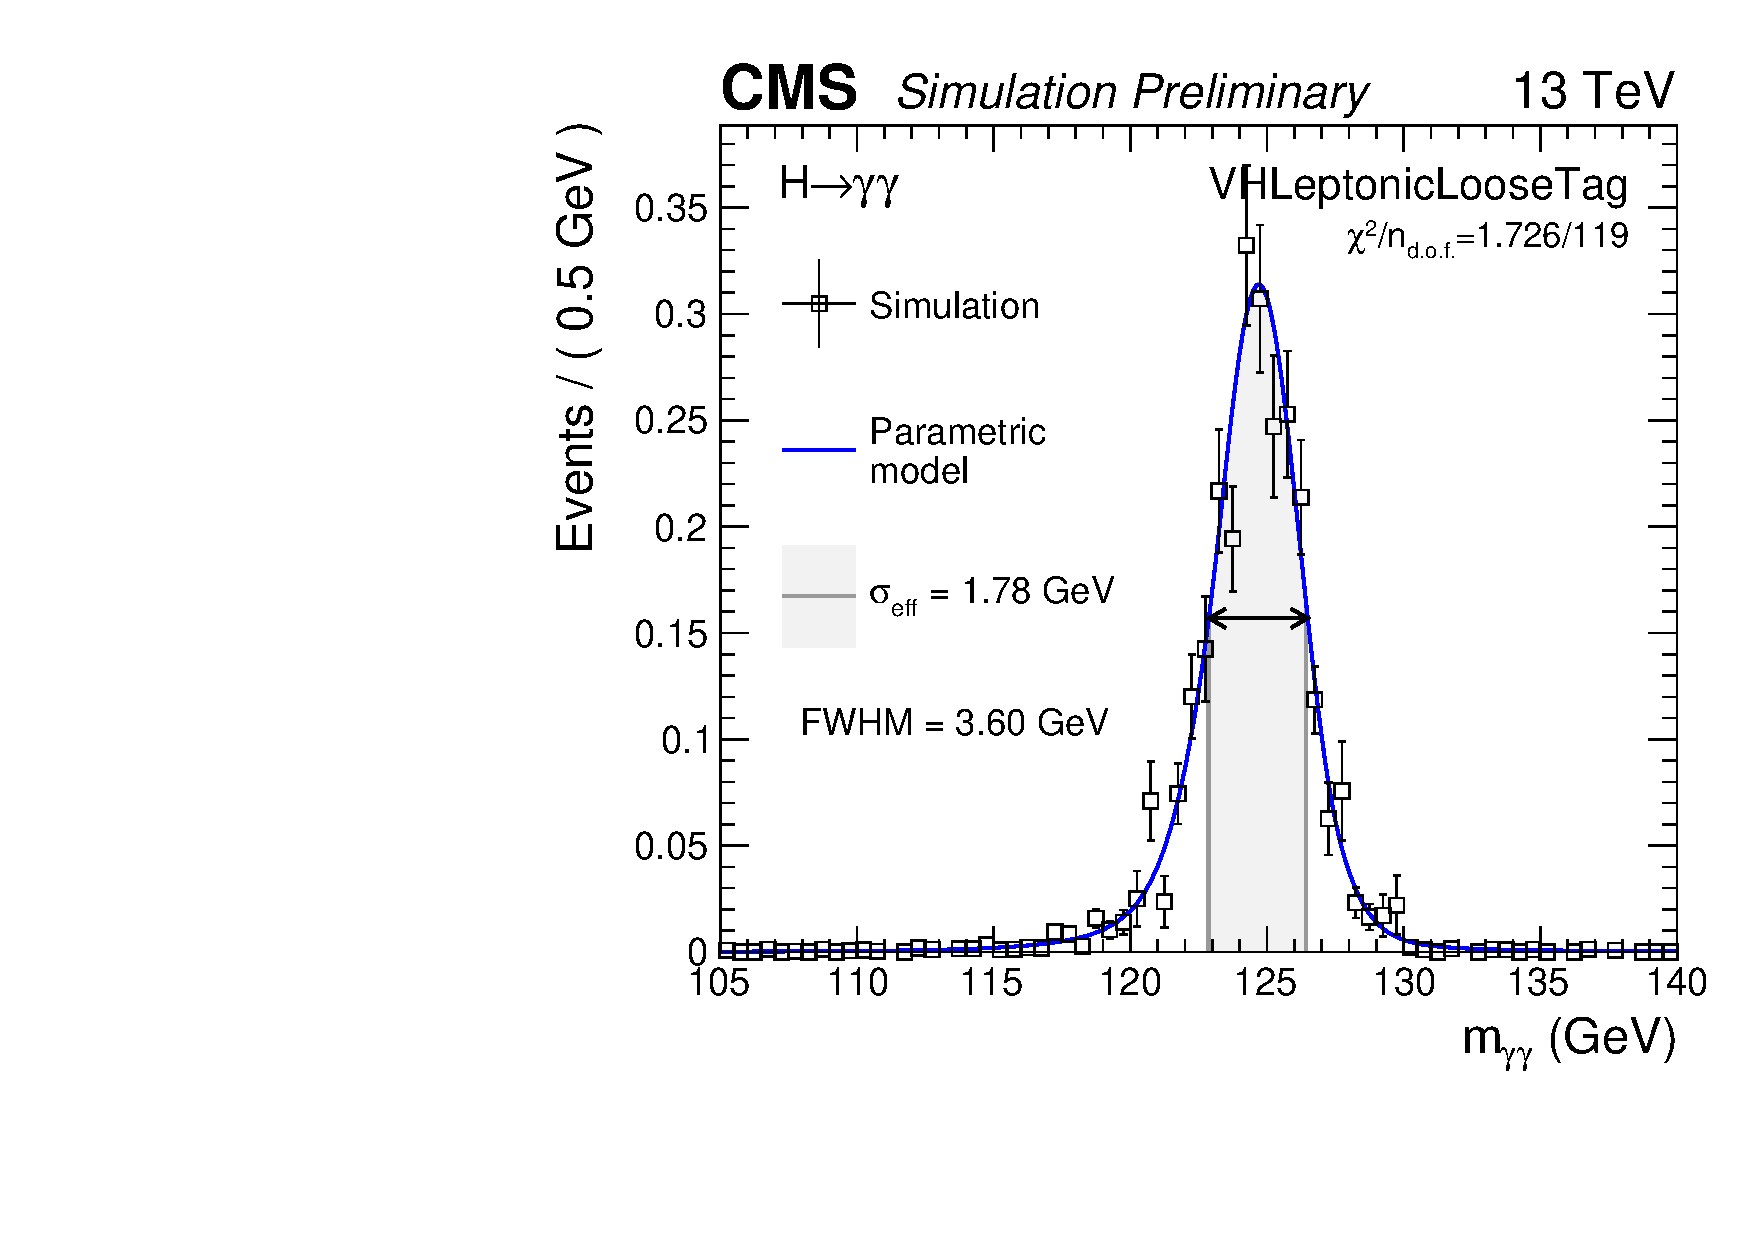
\includegraphics[width=0.45\textwidth]{modellingFigures/\whichFig/DCBpG/SSF/VHLeptonicLooseTag.pdf} 
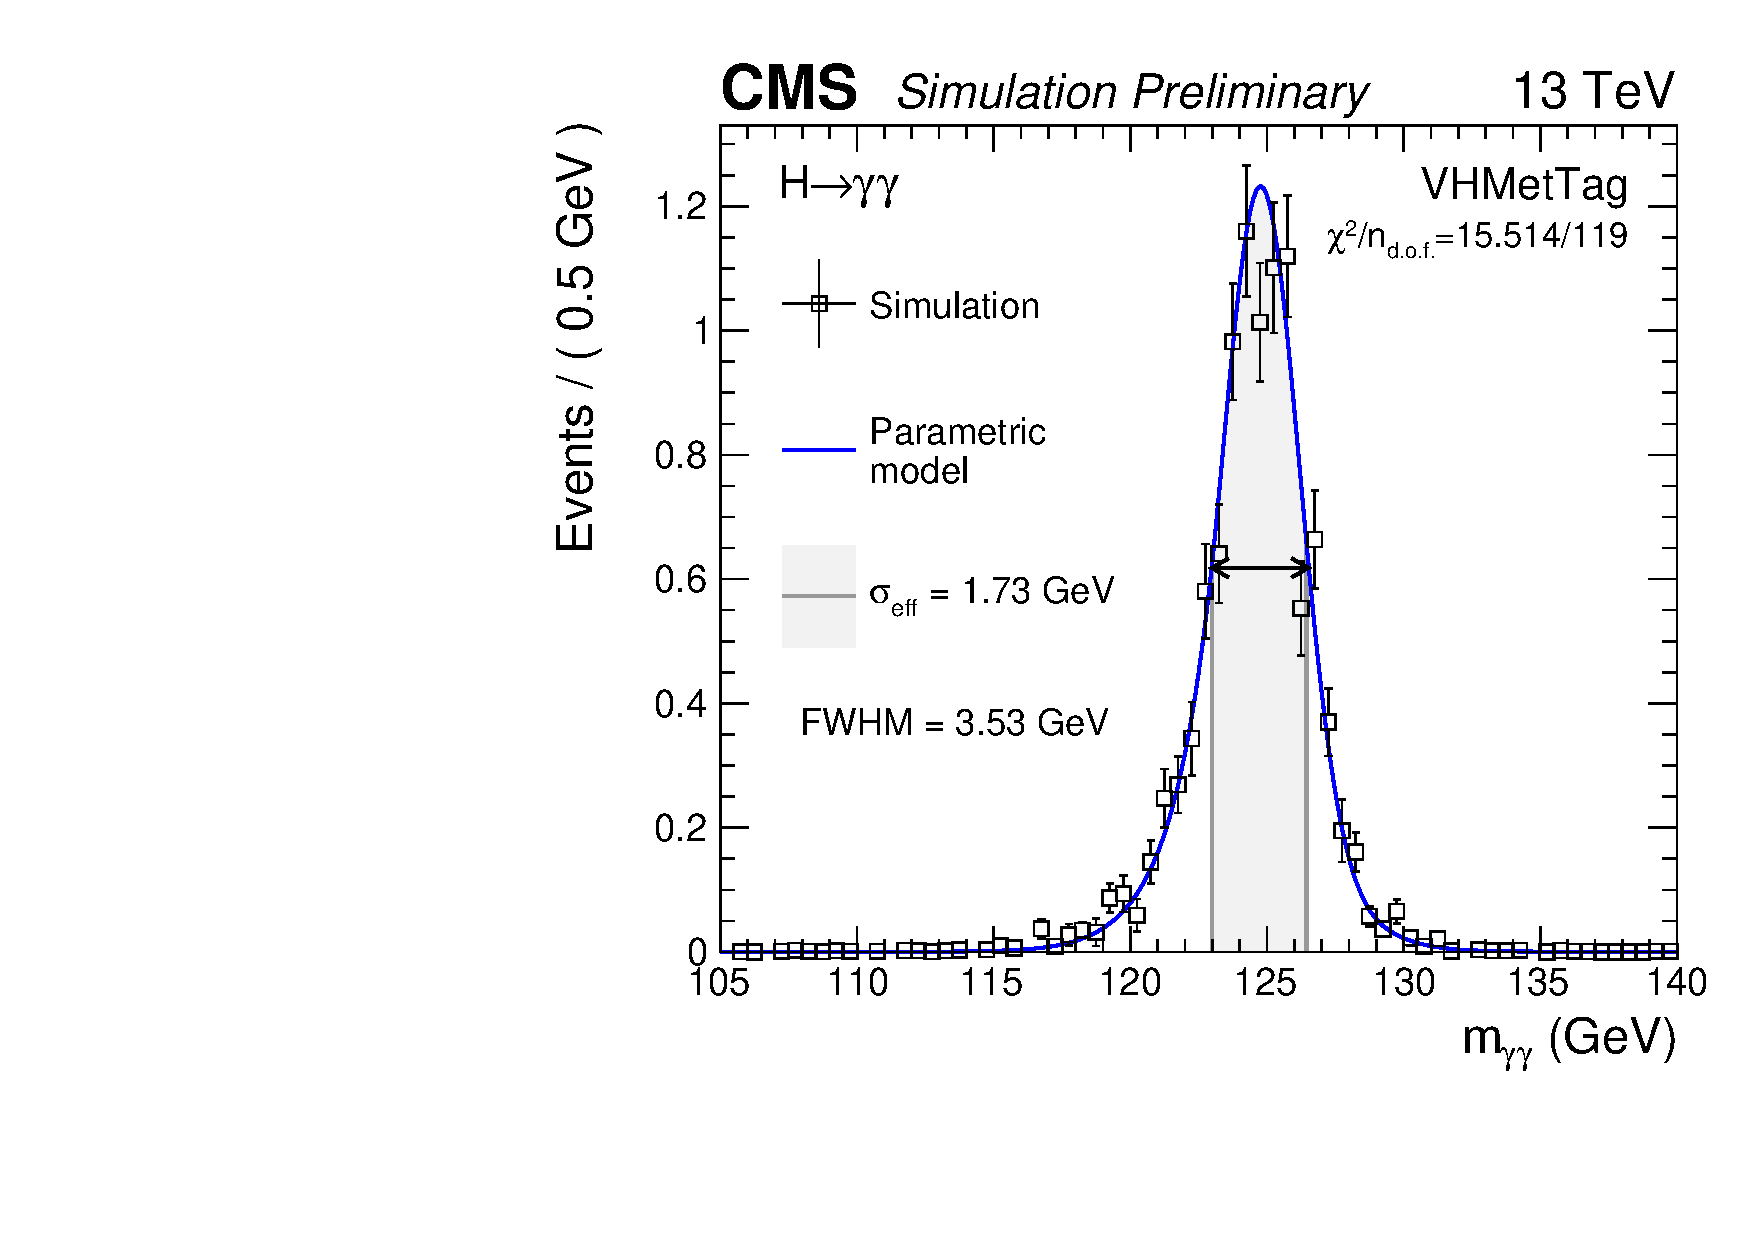
\includegraphics[width=0.45\textwidth]{modellingFigures/\whichFig/DCBpG/SSF/VHMetTag.pdf} \\
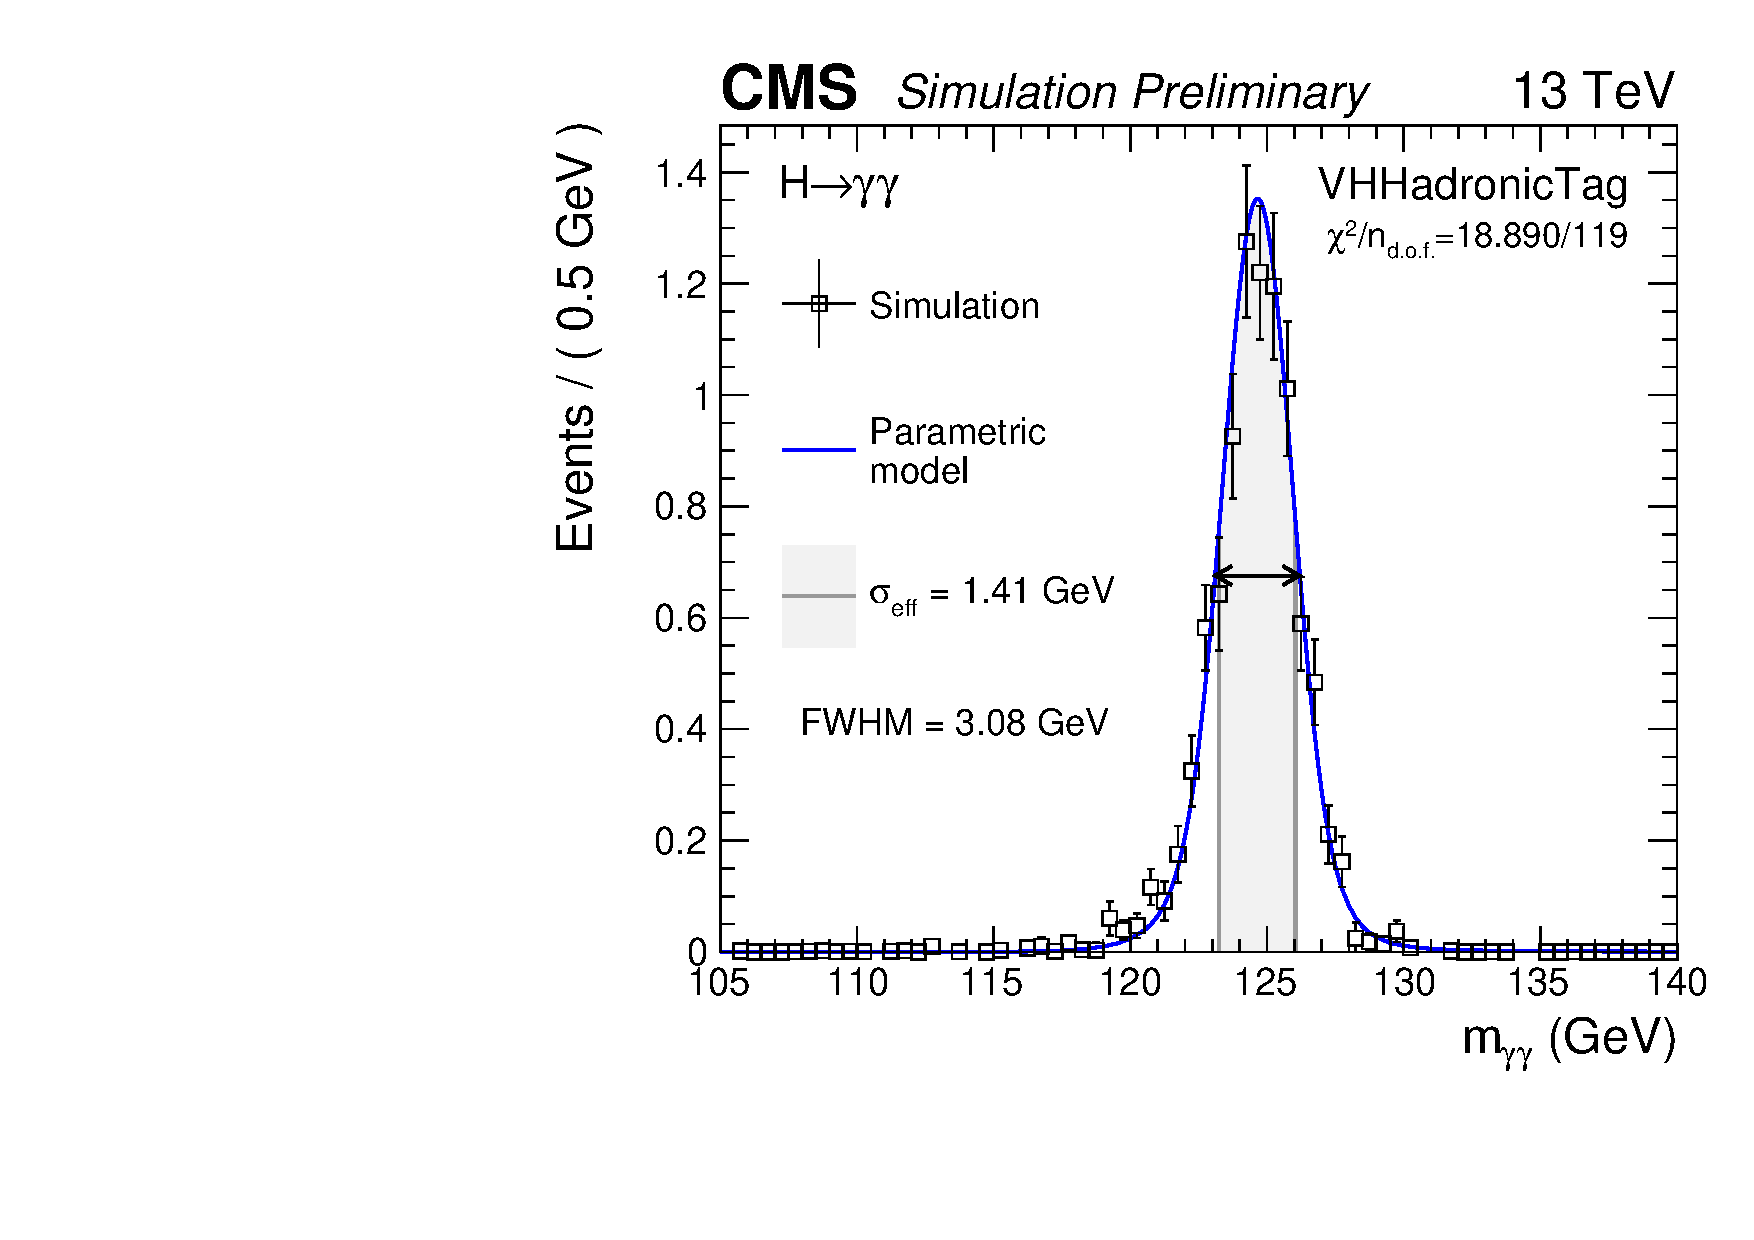
\includegraphics[width=0.45\textwidth]{modellingFigures/\whichFig/DCBpG/SSF/VHHadronicTag.pdf} 

\caption{The signal models for the \VHTag analysis categories for $\mH=125\GeV$, obtained by summing the contributions from each production process according to their \effxacc. The \effSigma (half the width of the narrowest interval containing 68.3\% of the invariant mass distribution) and the FWHM (the width of the distribution at half of the maximum value) are also shown.}

\label{fig:model:sig_model_per_category_tris}
\end{figure}
\fi
%\subsection{Handling of photon energy systematics}

%The systematics associa

\section{Background modelling}
\label{model:sec:background_model}
\subsection{The discrete profiling method}
\label{model:sec:background_model_envelope}

The background model is derived from data by fitting a function to the invariant mass spectrum in each category. However, the underlying functional form of a given background distribution is unknown. In some cases, several different families of function could in principle be chosen for the parametrisation, all giving acceptable agreement with the data. Even within a given family of functions, it is not always clear which to choose. The uncertainty associated with making a particular choice must be accounted for. %An common solution is to make an arbitrary choice of functional form and try to estimate the bias introduced by pikcing that shape, and trying to assign some systematic uncertainty to compensate.
These issues are addressed using the discrete profiling method~\cite{DiscreteProfiling}, which treats the choice of functional form as a discrete nuisance parameter in the final \NLL fit to the data. This method provides a natural way to include the uncertainty in the choice, and is described below.

When making a measurement of a parameter of interest using a \NLL minimisation, nuisance parameters representing systematic uncertainties are profiled: they are allowed to float during the minimisation, but their final value is not of interest. The additional freedom produces a wider \NLL curve, representing the additional uncertainty attributed to the floating nuisances. 
The same result can be obtained in a different way: if the value of one of the nuisance parameters is instead fixed at the best-fit value, the width of the resulting \NLL curve will be narrower but still with its minimum at the same place as the full profiled \NLL curve. This width represents the uncertainty of the measurement without the effect of the nuisance parameter in question. If the procedure is repeated for different fixed values of the nuisance parameter, different \NLL curves, not necessarily at the minimum, will be produced. In the limit that many different values of the fixed nuisance parameter are sampled, the minimum envelope of all the fixed-nuisance \NLL curves will converge to the full profiled \NLL curve. The uncertainty can then be obtained from the envelope as for a usual \NLL curve. This procedure is illustrated in \Fig~\ref{fig:model:bkg_envelope}, and can also be applied for nuisance parameters for which only some discrete, particular values are possible. When parametrising the background distribution, the chosen functional form can be treated as such a discrete nuisance parameter. The method described above can then be used to account for the uncertainty associated with the parametrisation of the background. The fact that different functional forms can have different numbers of parameters is taken into account by adding a penalty term to the \NLL proportional to the number of parameters in the function. 

\begin{figure}[ht!]
\centering
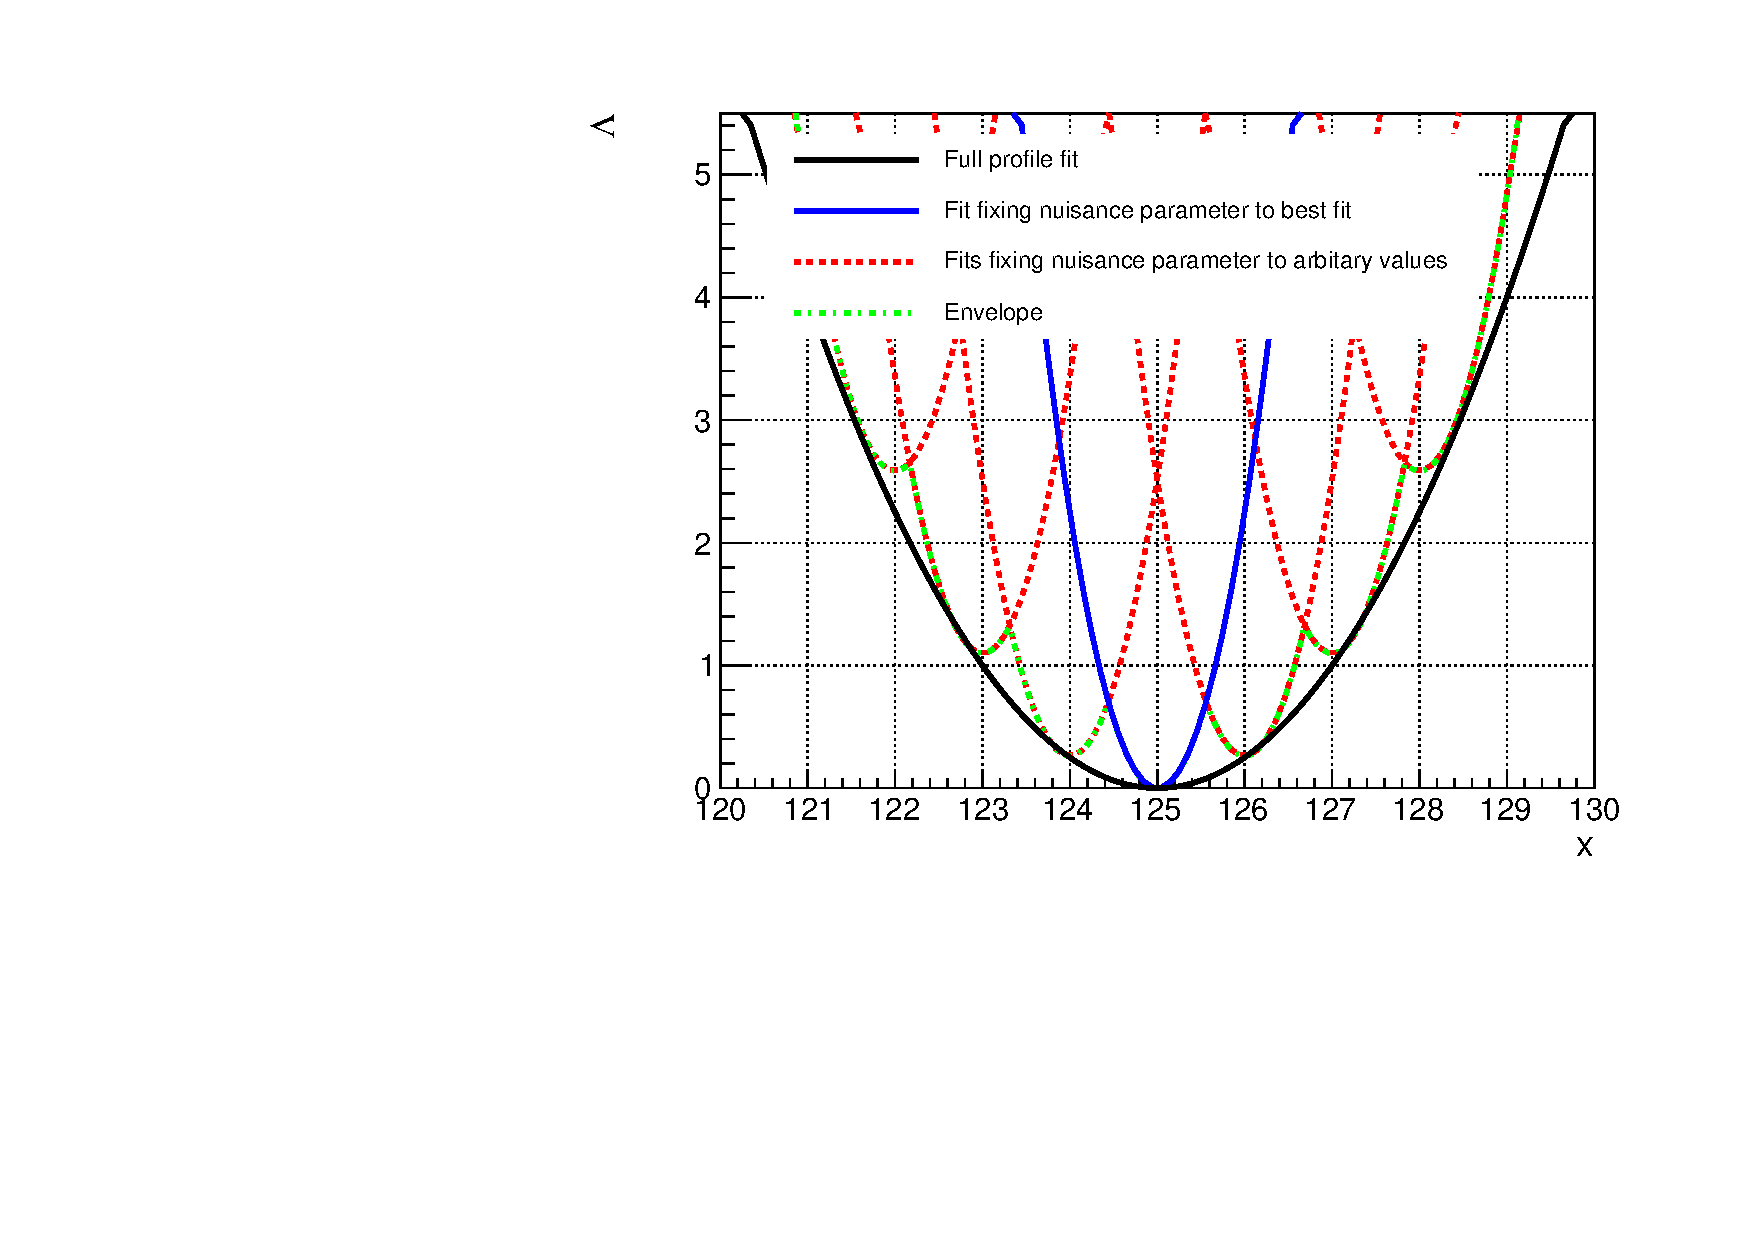
\includegraphics[width=0.9\textwidth]{modellingFigures/envelope_cartoon.pdf} 
\caption{An illustration of the construction of the envelope to estimate the effect of a nuisance parameter. The NLL (denoted as $\Lambda$) curve obtained when performing a likelihood scan of parameter of interest $x$ if the nuisance parameter is profiled is shown in black. The NLL curve obtained by fixing the nuisance to the best-fit value is shown in blue. The NLL curves for various fixed values of the nuisance other than the best-fit are shown in red. The minimum envelope of these curves, shown in green, approximates the original NLL curve obtained by profiling the nuisance parameter~\cite{DiscreteProfiling}.}

\label{fig:model:bkg_envelope}
\end{figure}

\subsection{Application in the \Hgg analysis}

In theory, a complete set of all analytic functions should be considered to obtain an exact result using the discrete profiling method. In practice, it is only necessary to include the subset of all analytic function which give a good description of the data. In this analysis, where the background distribution is smoothly falling, the following four families of functions are considered:
\begin{itemize}
\item sums of exponentials, $$ f_{N}(x)= \sum^{N}_{i=1} p_{2i-1} e^{p_{2i} x} ;$$
\item sums of polynomials (in the Bernstein basis), $$ f_{N}(x) = \sum^{N}_{i=0} p_{i} b_{(i,N)}, \text{ where } b_{(i,N)}:= \begin{pmatrix} N \\ i \end{pmatrix} x^i (1-x)^{N-i} ;$$
\item Laurent-type series, $$ f_{N}(x)= \sum^{N}_{i=1} p_{i} x^{-4 + \sum^{i}_{j=1} (-1)^{j} (j-1)};$$
\item sums of power-law functions: $$ f_{N}(x)= \sum^{N}_{i=1} p_{2i-1} x^{-p_{2i}};$$
\end{itemize}
where for all $k$, the $p_k$ are a set of parameters, and $N$ represents the order of a particular function in the family. 
%The representations of the function families are chosen such that their members are nested: a function of a particular order can reproduce the shape of the functions of lower order for a suitable choice of parameter values. It is therefore only necessary to consider a single representative function from each family when applying the discrete profiling method. 
In order to keep the computing time required for the fitting to a tolerable level, only a subset of functions from each family are considered. The maximum order of the candidate function considered from each family is obtained separately for each analysis category using the following procedure. Starting with the lowest-order function in the family, the parameters of the candidate function are varied to minimize the \NLL with respect to the $m_{\gamma\gamma}$ distribution. A penalty of $1$ times the number of parameters in the functional form is added to the value of the \NLL to account for differences in the number of parameters. The same procedure is applied to the function of next-highest order in the family. 
In the limit of large sample size, the difference in the minimum \NLL between functions of successive orders $N$ and $N+1$, $2 \Delta NLL_{N+1} = 2(NLL_{N+1} - NLL_{N})$, is distributed as a $\chi^2$ with $M$ degrees of freedom where, $M$ is the difference in the number of free parameters in the order-($N+1$) and order-$N$ functions. A \pvalue is then calculated as:

$$ \text{\pvalue} = \text{prob}(2 \Delta NLL > 2 \Delta NLL_{N+1}| \chi^2(M)). $$

If the \pvalue is less than a predetermined threshold, chosen as $0.05$, the higher-order function is supported by the data, otherwise the higher-order function is assumed unnecessarily flexible given the data. In the former case, the next-highest order function is then considered, and so on. Otherwise, the procedure terminates having found the highest-order suitable function. An additional constraint is applied to remove low order functions which do not fit the data well. These would not contribute to the minimum envelope anyway, and removing them reduces the amount of time needed to perform the final minimisation described in Chapter~\ref{chap:statandresults}. The remaining functions from each of the four families are added to the final set of candidate functions to be used in the discrete profiling. As an example, the chosen functions for the \Untagged categories are shown in \Fig~\ref{fig:model_bkg_multipdf}. The equivalent figures for the other analysis categories are available in \App~\ref{app:modelling} in \Fig~\ref{fig:model_bkg_multipdf_bis}. For each category, the candidate functions give acceptable agreement with the data, but can lead to large variations in the predicted number of events in the region of interest between $120$ and $130\GeV$. %and~\ref{fig:model:bkg_multipdf_bis}.

A series of tests demonstrated that this method provides good coverage of the uncertainty associated with the choice of the function and provides an unbiased estimate of the signal strength. These tests are described in detail in~\cite{DiscreteProfiling}. 

\begin{figure}[p]
 \begin{center}
 \subfloat[\Untagged 0]{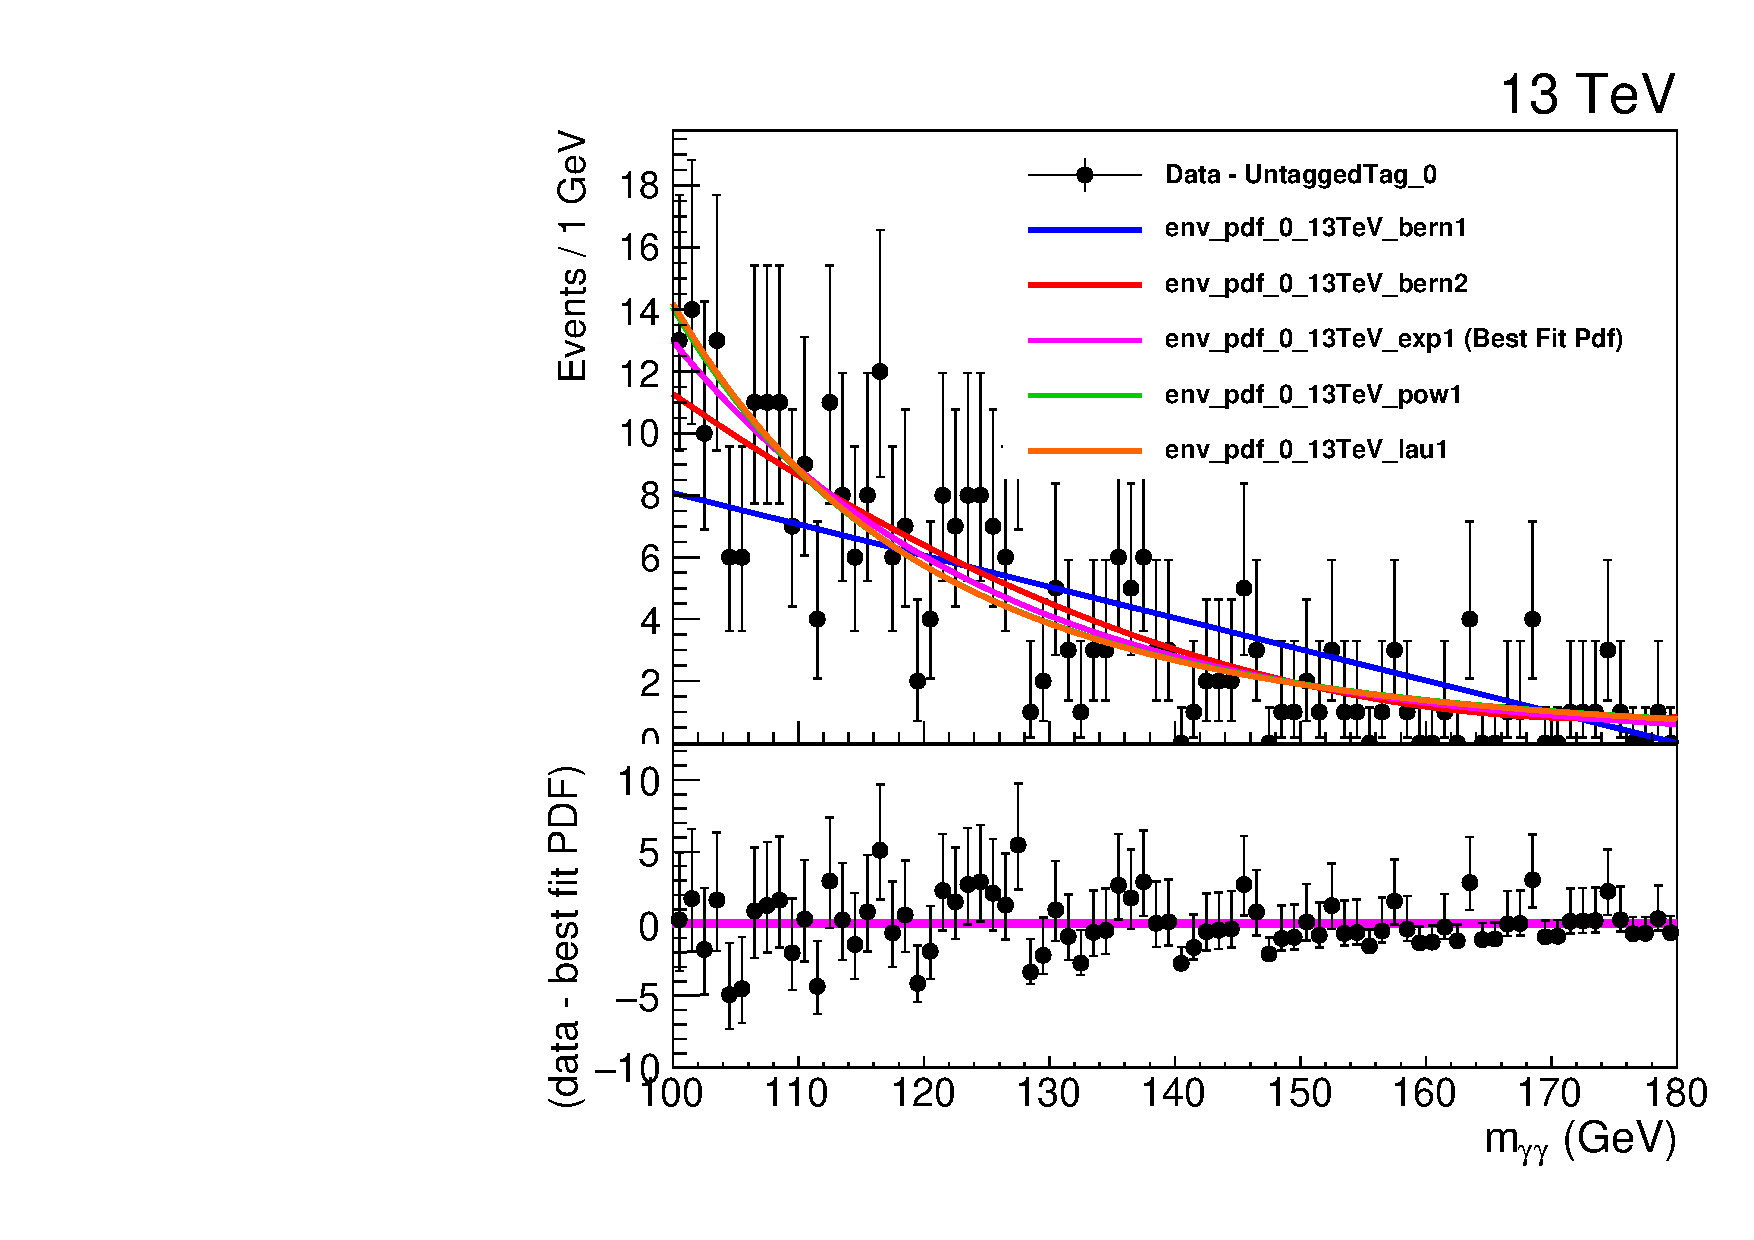
\includegraphics[width=0.45\textwidth]{modellingFigures/\whichFig/multipdf/multipdf_UntaggedTag_0.pdf}}
 \subfloat[\Untagged 1]{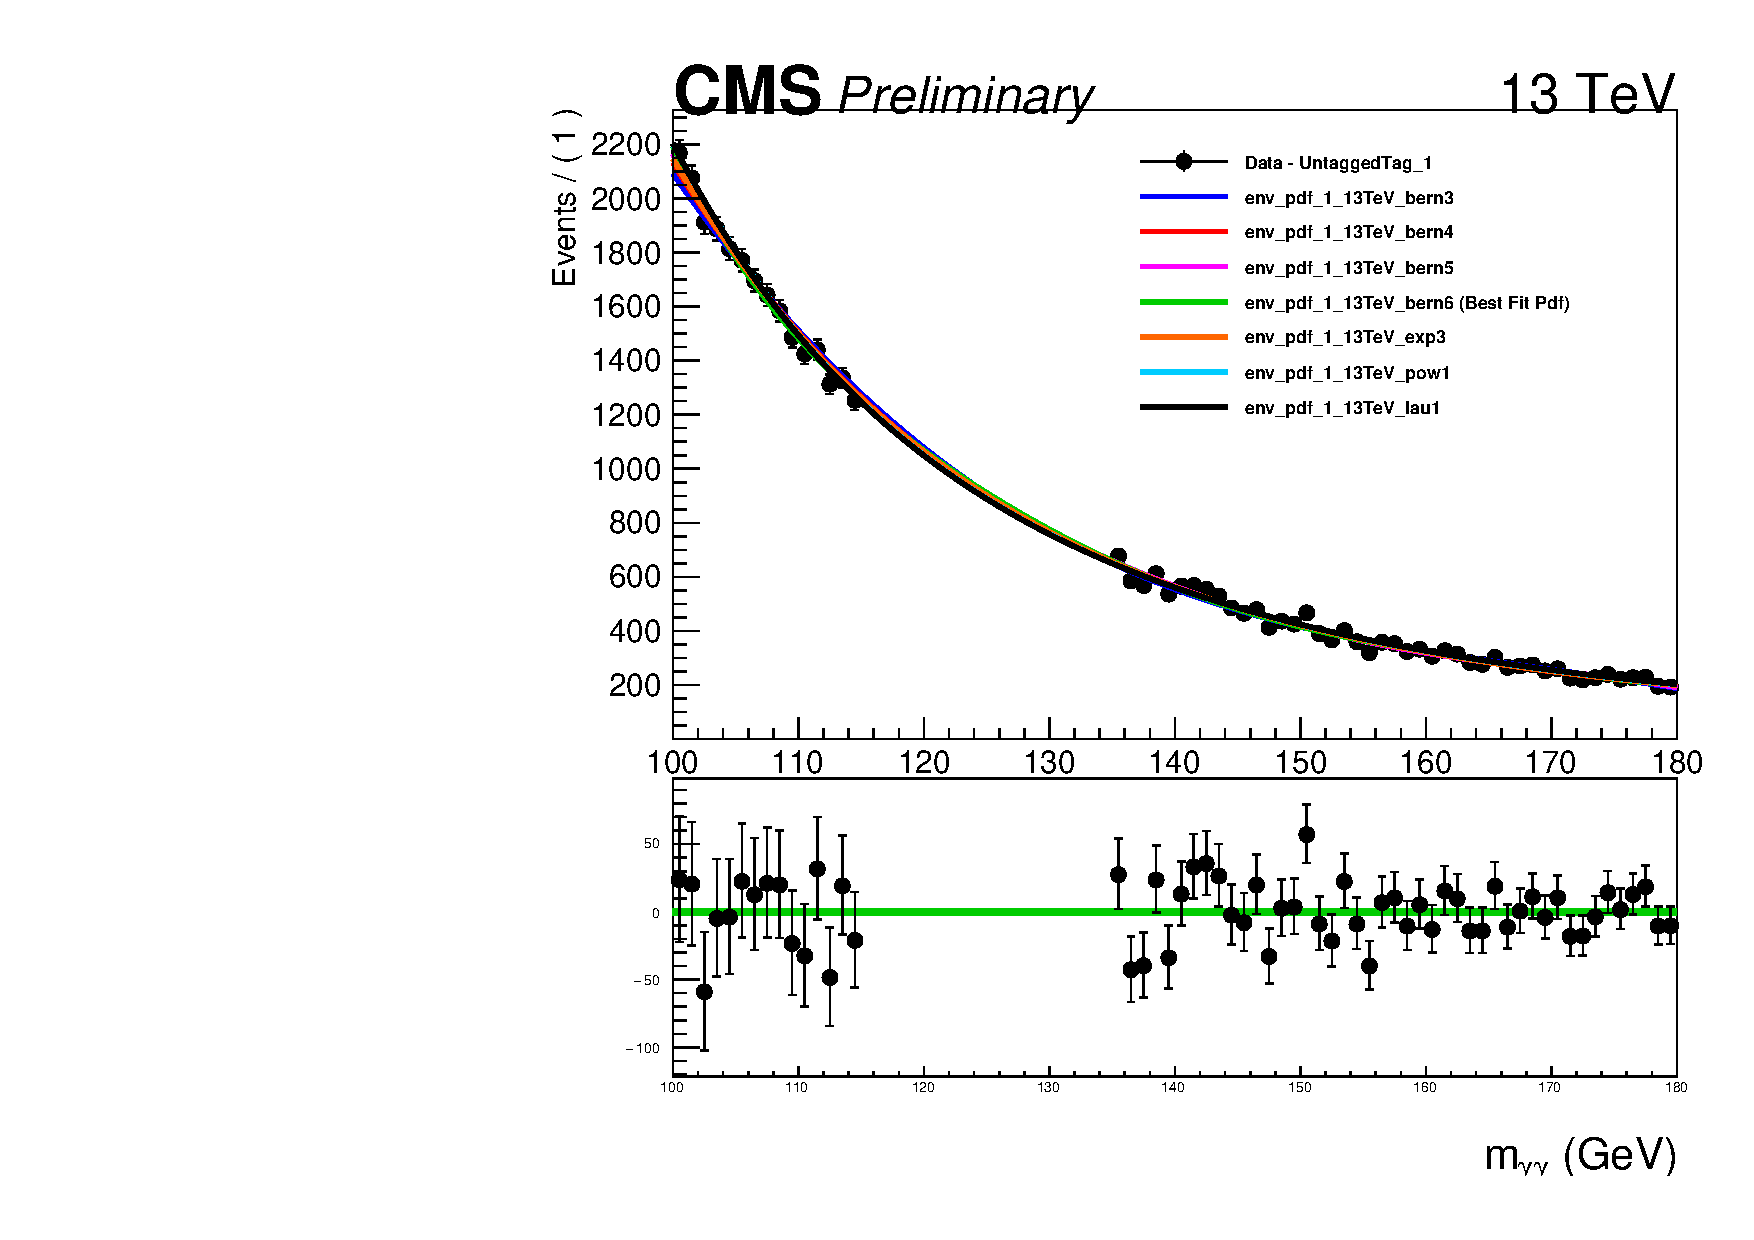
\includegraphics[width=0.45\textwidth]{modellingFigures/\whichFig/multipdf/multipdf_UntaggedTag_1.pdf}}\\
 \subfloat[\Untagged 2]{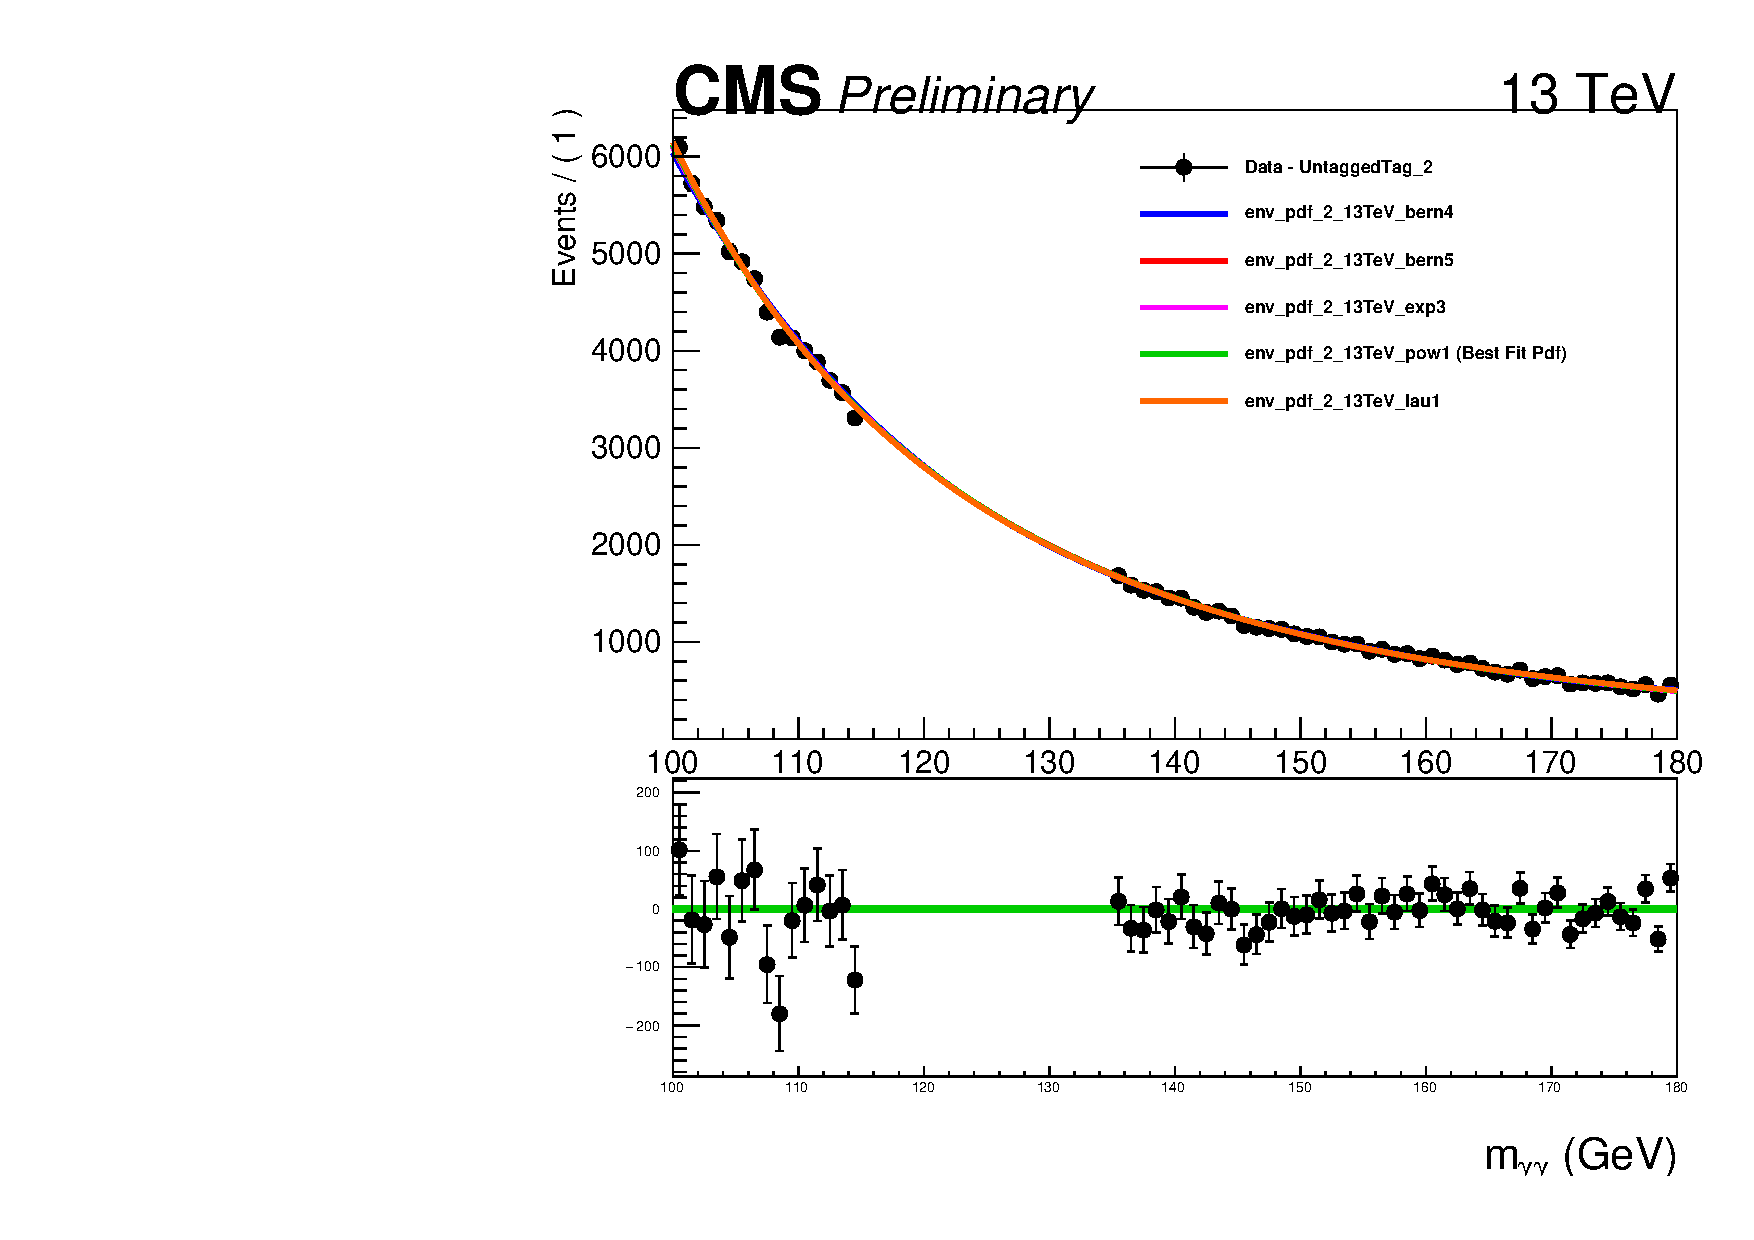
\includegraphics[width=0.45\textwidth]{modellingFigures/\whichFig/multipdf/multipdf_UntaggedTag_2.pdf}}
 \subfloat[\Untagged 3]{\includegraphics[width=0.45\textwidth]{modellingFigures/\whichFig/multipdf/multipdf_UntaggedTag_3.pdf}}\\
% \subfloat[\VBFTag 0] {\includegraphics[width=0.3\textwidth]{modellingFigures/\whichFig/multipdf/multipdf_VBFTag_0.pdf}}
% \subfloat[\VBFTag 1] {\includegraphics[width=0.3\textwidth]{modellingFigures/\whichFig/multipdf/multipdf_VBFTag_1.pdf}}
% \subfloat[\VBFTag 2] {\includegraphics[width=0.3\textwidth]{modellingFigures/\whichFig/multipdf/multipdf_VBFTag_2.pdf}}
 \caption{The set of candidate functions chosen to parametrise the background using the discrete profiling method in the \Untagged categories. For each category, all candidate functions give acceptable agreement with the data, but can lead to large variations in the predicted number of events in the region of interest between $120$ and $130\GeV$. The resulting uncertainty in the choice of parametrisation is handled by the discrete profiling method.}
 \label{fig:model_bkg_multipdf}
 \end{center}
\end{figure}

%\begin{figure}
% \begin{center}
% \subfloat[\TTHLeptonicTag]{\includegraphics[width=0.3\textwidth]{modellingFigures/\whichFig/multipdf/multipdf_TTHLeptonicTag.pdf}}
% \subfloat[\TTHHadronicTag]{\includegraphics[width=0.3\textwidth]{modellingFigures/\whichFig/multipdf/multipdf_TTHHadronicTag.pdf}}\\
% \subfloat[\TTHLeptonicTag]{\includegraphics[width=0.3\textwidth]{modellingFigures/\whichFig/multipdf/multipdf_VHLeptonicLooseTag.pdf}}
% \subfloat[\TTHHadronicTag]{\includegraphics[width=0.3\textwidth]{modellingFigures/\whichFig/multipdf/multipdf_VHMetTag.pdf}}
% \subfloat[\TTHLeptonicTag]{\includegraphics[width=0.3\textwidth]{modellingFigures/\whichFig/multipdf/multipdf_VHHadronicTag.pdf}}\\
% \subfloat[\TTHHadronicTag]{\includegraphics[width=0.3\textwidth]{modellingFigures/\whichFig/multipdf/multipdf_WHLeptonicTag.pdf}}
% \subfloat[\TTHHadronicTag]{\includegraphics[width=0.3\textwidth]{modellingFigures/\whichFig/multipdf/multipdf_ZHLeptonicTag.pdf}}
% \caption{The set of candidate functions chosen to parametrise the background using the discrete profiling method in the \TTHTag and \VHTag categories.} 
% \label{fig:model:bkg_multipdf_bis}
% \end{center}
%\end{figure}


\section{Systematic uncertainties}
\label{model:sec:systematics}

The systematic uncertainty on the choice of the background fitting function is handled directly by the discrete profiling method described in \Sec~\ref{model:sec:background_model}. The uncertainties which affect the signal model are more numerous, and are implemented according to their effect.

Systematic uncertainties which affect the shape of the \mgg distribution are built directly into the signal models described in \Sec~\ref{model:sec:signal_model}. Most systematics of this type impact individual photon energies, and therefore the invariant mass. The effect of the systematic variation is propagated to the mean, \effSigma and normalisation of the signal \mgg distribution for each category and signal process. Corresponding nuisance parameters are then inserted which can modify the normalisation, mean and width of the \DCBpG parametrisations. An exception is the nuisance corresponding to the vertex efficiency, which instead modifies the relative mixing fraction of the \RV and \WV components of the model. The nuisance parameters are then Gaussian-constrained and allowed to be profiled in the final \NLL minimisation when making measurements of the parameters of interest. Nuisances of this type are referred to hereafter as \emph{shape nuisances}. 

Uncertainties on selection efficiencies do not affect the shape of the \mgg distribution, but do change the final event count (or \emph{yield}) of the signal model for each category. Depending on the source of the systematic uncertainty, individual categories can be scaled differently, although all categories will simultaneously either increase or decrease. The corresponding nuisance parameters are profiled in the \NLL minimisation with a \lnN~\cite{1987lognormal} constraint, which cannot give rise to negative yields. Systematics of this type are referred to as \emph{yield nuisances}, which are either symmetric or asymmetric. %In the symmetric case, the upward and downward variations of the uncertainty are the same size. In the asymmetric case, the upward and downward variations are of different sizes.

Finally, some uncertainties affect the categorisation of events. In this case, the systematic variations can cause events to move from one event category to another, or altogether out of the acceptance of the analysis. These systematic uncertainties are implemented as nuisance parameters which change the relative yield of event categories, and are referred to as \emph{category migration nuisances}. They are implemented analogously to yield nuisances, except that the yield of certain categories will increase while the yield of others must decrease in turn. Furthermore, separate nuisances are implemented to account for different types of migration: for instance, between the individual \VBFTag categories on the one hand, and then between all \VBFTag and all \Untagged categories on the other.

%The source and evaluation of the various systematic uncertainties are described below.

\subsection{Theory uncertainties}
\subsubsection{Parton Distribution Functions}

The uncertainty on signal process \crosssection\s due to uncertainties on each \PDF produces both an overall change in signal yield and category migrations.

One symmetric yield nuisance for each signal process is included, accounting for both the uncertainties in the \PDF\s and the uncertainty on the strong force coupling constant (\alphaS). Each varies the category yields according to the corresponding uncertainty in the process \crosssection, as provided by the \LHCHXSWG recommendation~\cite{LHCHXSWGYR4}. Specifically, the \ggH, \VBF, \WH, \ZH, and \ttH process \crosssection\s are scaled by 3.2\%, 2.1\%, 1.9\%, 1.6\% and 3.6\% respectively. 

The relative yield change is modelled using a series of category migration nuisances. The size of the variations is determined according to the PDF4LHC prescription~\cite{Demartin:2010er}, by reweighting individual events according to the NNPDF30 \PDF set~\cite{Carrazza:2015aoa}. The effect of the variations is normalised by their effect on the overall yield in each category, such that they represent only migrations. The procedure results in 60 uncorrelated symmetric category migration nuisances. 
The migrations are of the order of 0.5\% in most categories.

\subsubsection{QCD scale}
The uncertainty on the scale of the \QCD interaction is parametrised in terms of the renormalisation ($\mu_{R}$) and factorisation ($\mu_{F}$) scales. The asymmetric yield nuisances corresponding to variations of these parameters are taken direction from the \LHCHXSWG recommendations for \crosssection\s~\cite{LHCHXSWGYR4}. The size of the effect for the \ggH, \VBF, \WH, \ZH and \ttH processes is $^{+4.6\%}_{-6.7\%}$, $^{+0.4\%}_{-0.3\%}$, $^{+0.5\%}_{-0.7\%}$, $^{+3.8\%}_{-3.0\%}$ and $^{+5.8\%}_{-9.2\%}$ respectively. 

Three additional asymmetric category migration nuisances are also included. The size of their effect is estimated at generator level, by varying the values of $\mu_{R}$ and $\mu_{F}$ by factors of $2$ (upward variation) or $0.5$ (downward variation). The three category migration nuisances correspond to: varying $\mu_{R}$ up or down while keeping $\mu_{F}$ constant; varying $\mu_{F}$ up or down while keeping $\mu_{R}$ constant; and varying both $\mu_{R}$ and $\mu_{F}$ up or down uniformly. In each case the migrations are found to be of the order of 1-4\% of the category yield.


\subsubsection{Strong force coupling constant}
The effect of the uncertainty on the value of \alphaS is modelled as described in the section for the uncertainties on the \PDF\s. The yield nuisances for the uncertainties on the \PDF\s also incorporate the uncertainty on \alphaS. Three additional asymmetric category migration nuisances are included, the effects of which are determined according to the PDF4LHC prescription~\cite{Demartin:2010er}.  
The migrations are of the order of 0.5\% in most categories.

\subsubsection{\Hgg branching ratio}
The uncertainty on the \SM \Hgg branching fraction is taken directly from~\cite{LHCHXSWGYR4}. It is implemented as a yield nuisance affecting all analysis categories, and the variation is of 2.08\% on the category yield.

\subsubsection{Gluon fusion contamination of \VBFTag and \TTHTag categories}
The theoretical prediction for the jet multiplicity in gluon fusion events is unreliable for high multiplicities. This leads to the introduction of an uncertainty on the contamination of \ggH events in other analysis categories which use jets in their selections. 

For \VBFTag categories, the uncertainty is estimated using the Stewart-Tackmann procedure~\cite{StewartTackmann}. This results in a set of category migration nuisances: a migration between \VBFTag categories (at most $39\%$ on category yield) and a migration between \Untagged and \VBFTag categories (at most $10\%$ on category yield); %jetveto

For the \TTHTag categories, the equivalent effect is modelled with yield nuisances instead of categorisation migration nuisances. This is because there is no migration between the two \TTHTag categories, and the effect of migrating events into the \Untagged categories would be negligible. Three yield nuisances are considered, which represent:
\begin{itemize}
\item parton shower modelling uncertainty, which is estimated by comparing the jet multiplicity in data and simulation for $\Ptop \APtop \rightarrow \text{jets}$ events, where the top quarks both decay to leptons, leading to variations of the order of 45\% on the yield of the \TTHTag categories; 
\item ``gluon splitting'' modelling, which is estimated from the ratio of \crosssection\s of $\Ptop \APtop \Pbottom \APbottom$ and $\Ptop \APtop +2\text{ jet}$ events in 13\TeV data. The size of this variation is of the order of 18\% on the yield of the \TTHTag categories;
\item an additional nuisance included to account for the small size of the simulated samples used in these studies. The size of this variation is of the order of 10\% on the yield of the \TTHTag categories.
\end{itemize}

\subsubsection{Underlying event and parton shower modelling}
%The uncertainty on the \emph{underlying event} is introduced because 
%Different models exist to describe the interactions of quarks and gluons in \pp collisions, each giving different predictions for the topology, energy and number of jets in the events. Two main sources of uncertainty exist as a result of these different models: the uncertainties related to the modelling of the \emph{underlying event} and the \emph{parton shower}.
\ifNewAnalysis
The \emph{underlying event} refers to all the soft interactions between partons which occur in addition to the hard scatter in a \pp collision. In the \Pythia~\cite{Pythia8} simulations used for this analysis, this modelled as multiple independent scatterings between the other partons. Tuning the parameters of the modelling of the underlying event can lead to a modified jet production \crosssection, which can affect the categorisation of \VBF events. This uncertainty is therefore taken into account as a set of category migration nuisances. The sizes of the variations are obtained from dedicated simulated samples where the parameters relating to the underlying event (such as the momentum cutoff for such additional interactions, and the matter density of the proton) have been tuned differently. The category migrations evaluated are between: \VBFTag 0 and \VBFTag 1  categories (of the order of 7\%); \VBFTag 0-1  and \VBFTag 2 categories (of the order of X\%); and all \VBFTag categories and all \Untagged categories (of the order of 9\%).

\emph{Parton shower} modelling refers to the emission of \QCD radiation in the form of gluons from partons during \pp collisions. These gluons can themselves emit further \QCD radiation or convert to quark-antiquark pairs, until hadronisation occurs. The modelling of these showers depends on certain parameters, such as the hadronisation scale, which is not known. This can affect the shape, number or energy of jets, and so the \VBF categorisation. The uncertainty is therefore treated as a set of category migrations nuisance between: \VBFTag 0 and \VBFTag 1 categories (of the order of 7\%); \VBFTag 0-1  and \VBFTag 2 categories (of the order of X\%); and all \VBFTag categories and all \Untagged categories (of the order of 9\%).
\else
The \emph{underlying event} refers to all the soft interactions between partons which occur in addition to the hard scatter in a \pp collision. In simulation, these are modelled as multiple independent scatterings between the other partons. Tuning the parameters of the modelling of the underlying event (such as the momentum cutoff for such additional interactions, and the matter density of the proton) can lead to a modified jet production \crosssection. %, which can affect the categorisation of \VBF events. 

\emph{Parton shower} modelling refers to the emission of \QCD radiation in the form of gluons from partons during \pp collisions. These gluons can themselves emit further \QCD radiation or convert to quark-antiquark pairs, until hadronisation occurs. The modelling of these showers depends on certain parameters, such as the hadronisation scale, which is not predicted perturbatively. 

Both of these uncertainties can affect the shape, number or energy of jets, and so the \VBF categorisation. The sizes of the variations are obtained from dedicated simulated samples where the parameters relating to the underlying event and parton shower modelling have been tuned differently. The uncertainties are treated together as a set of category migrations nuisance between: \VBFTag 0 and \VBFTag 1 categories (of the order of 8\%); and all \VBFTag categories and all \Untagged categories (of the order of 9\%).
\fi
\subsection{Photon uncertainties}

\subsubsection{Photon preselection}
The efficiency of the photon preselection is quantified using the \TagAndProbe method described in \Sec~\ref{reco:sec:pho:preselection}, which also provides systematic uncertainties for different photon classes. The systematic uncertainties are propagated to a yield nuisance, the effect of which is around 4\% on the category yields.

\subsubsection{Photon identification}
An uncertainty on the photon identification efficiency is introduced to account for the difference in distributions of the \PhoIdBdt output score observed between data and simulation in \Zee events (see \Fig~\ref{fig:reco:photon_id_zee_validation}). The size of this uncertainty is approximately $3\%$ on the value of the output score. This is treated as a yield nuisance, where the uncertainty on the output score is translated to an uncertainty on the yield of the order of $3\%$. 

\subsubsection{Photon energy scale and resolution}
After the calibration of the \ECAL described in \Sec~\ref{sec:cms:ecal:calibration}, there are still some discrepancies in the photon energy scale and resolution between simulation and data. Since electrons and photons are both reconstructed as \SC\s, these discrepancies can be studied using \Zee events where the electrons are reconstructed as photons.
For \SC\s in eight \RNINE and $|\eta|$ classes, the invariant mass distributions in data and simulation are both fitted with a \BW function convoluted with a \CB function. The \BW function models the natural shape of the \PZ-peak, while the \CB function describes the \ECAL resolution and losses due to unrecovered energy from bremsstrahlung. The natural width and pole mass of the $\PZ$ boson are fixed to their accepted values~\cite{PDGBooklet} in this parametrisation. 

The corrections to the photon energy scale are given by the relative differences between the best-fit means of the \CB in data and simulation, divided by the $\PZ$ boson pole mass, in each bin. The corrections to the photon energy resolution are applied by adding additional smearing terms to the width of the \CB in quadrature. The additional scale and resolution corrections described above each have uncertainties, which are related to choices made for the \Zee event selection and classification, as well as the difference between the final electron and photon energy regression \BDT\s. The uncertainties on the energy scale and resolution are quantified for each photon class, and propagated to the \mgg distribution in each analysis category. This results in shape nuisances for the photon energy scale in four classes (high and low \RNINE, each for \EB and \EE), and eight shape nuisances for the photon energy smearing (parametrised as constant and stochastic contributions). 

The size of the systematic uncertainties are of the order of 0.15\% to 0.50\% depending on the photon class. The effect on the mean of the \mgg distribution is at most 0.25\%, while the effect on the \effSigma is at most 20\%, depending on the analysis category.

\subsubsection{Per-photon energy resolution}
The uncertainty of the per-photon energy resolution is conservatively evaluated by scaling the output of the \PhoEnergyBdt described in \Sec~\ref{sec:reco:photon:phoenergybdt} by $\pm5\%$. This uncertainty is propagated throughout the analysis and modelled as a yield nuisance. The size of the variation is typically of the order of 2\% depending on the analysis category.

\subsubsection{Non-linearity of detector response}
The uncertainty associated with the fact that the \ECAL response is not linear is estimated by comparing boosted \Zee decays in data and simulation. Individual photon energies are affected by up to 0.2\%. The effect is propagated as a shape nuisance, which varies the mean of the \mgg distribution by 0.1\% in each category.

\subsubsection{Shower shape corrections}
The uncertainty deriving from the imperfect modelling of shower shape variables is estimated using simulated samples with and without the corrections. This effect is of order 0.06\% on the photon energy scale, and is implemented as four shape nuisances for photons in different $\eta$ and \RNINE classes, which vary the \mgg distribution mean by at most 0.20\% and \effSigma by at most 1.80\%.

\subsubsection{Non-uniformity of the light collection}
The uncertainty on the response of the \ECAL crystals depending on their position in \eta is modelled separately as shape nuisances for photons in the barrel and in the endcaps. The size of the uncertainty is 0.07\% on the photon energies. The effect is propagated to the \mgg distribution of each category and applied as separate shape nuisances in the \EE and \EB, which vary the mean by up to 0.2\% and the \effSigma by up to 5\%.

\subsubsection{Modelling of detector response in \Geant}
Imperfect modelling of the differences between electromagnetic showers for electrons and photons in the detector simulation software \Geant may have a small impact on the photon energy scale. The size of the variation is determined with a dedicated simulated sample where the parameters of shower modelling are modified. The size of the effect is found to be consistent with zero, but an upper bound of approximately 0.05\% is applied on the uncertainty on the mean of the \mgg distribution in each category.

\subsubsection{Modelling of the material budget}
The imperfect modelling of the amount of material between the vertex and the \ECAL affects the simulation of the photon and electron showers. The uncertainty related to this effect is estimated with dedicated samples where the amount of simulated material is uniformly varied by $\pm 5\%$. It is treated as two separate shape nuisances, for \EB and \EE photons separately, which affect the mean of the \mgg distribution by at most 0.1\% (0.03\%) and the \effSigma by at most 3.5\% (7.6\%) for the \EB (\EE) photons.

\subsubsection{Electron veto}
The electron veto element of the photon preselection is validated separately using \Zmmg events. A small uncertainty is introduced to account for the discrepancy between data and simulation. This source of uncertainty is treated as a yield nuisance, the size of which is of the order of 0.5\%. 

\subsection{Per-event uncertainties}

\subsubsection{Integrated luminosity}
\ifNewAnalysis
The uncertainty on the value of the integrated luminosity of the data sample is modelled as a scale nuisance, the size of which is 2.5\% on the yield of all signal processes. 
\else
The uncertainty on the value of the integrated luminosity of the data sample is modelled as a scale nuisance, the size of which is 6.2\% on the yield of all signal processes. 
\fi

\subsubsection{Jet energy scale and resolution}
The uncertainties on the jet energy scale are described by category migration nuisances: between \VBFTag 0 and \VBFTag 1 (typically of order 3\% on the category yield); between all \VBF and \Untagged categories (of order 10\%); and between \TTHTag and \Untagged categories (of order 12\%).

The nuisances for the jet energy resolution are treated analogously, with migrations of order 0.5\% between \VBFTag 0 and \VBFTag 1 categories; of order 1.5\% between \VBF and \Untagged categories; and of order 4\% between \TTHTag and \Untagged categories.

\subsubsection{Diphoton selection}
The \DiPhoBdt output score is used to make a selection on the diphotons which enter the analysis. A small uncertainty is introduced to account for the residual discrepancy between data and simulation in \Zee events after the uncertainties from the estimate of the per-photon energy resolution and the \PhoIdBdt score are taken into account. This source of uncertainty is treated as a yield nuisance, the size of which is 0.2\% in all categories. 

\subsubsection{Vertex-finding efficiency}
The uncertainty on the vertex-finding efficiency is determined by comparing the fraction of correctly identified vertices in \Zmumu between data and simulation. The uncertainty is modelled as a shape nuisance which alters the \RV/\WV mixing fraction of each signal model. 
\ifNewAnalysis
The variation is of the order of 2\% on the \RV fraction.
\else
The variation is of the order of 1.5\% on the \RV fraction.
\fi

\subsubsection{Trigger efficiency}
The uncertainty on the trigger efficiency is estimated using a \TagAndProbe method as described in \Sec~\ref{sec:reco:data}. The uncertainty is applied as a yield nuisance parameter of size 0.1\%.

\subsubsection{Lepton reconstruction and $\Pbottom$-tagging efficiencies}
The uncertainty on the reconstruction of electrons and muons is determined by considering the ratio of leptons reconstructed in data and simulation. The result is implemented as a yield uncertainty for the \TTHTag categories of the order of 1\% for electrons and 5\% for muons.
\ifNewAnalysis
Similarly, the uncertainty on the tagging of $\Pbottom$ jets is evaluated by varying the ratio between the measured $\Pbottom$-tagging efficiency in data and simulation within their uncertainty. This is propagated to a yield nuisance, which has an effect of the order of 5\% for \TTHTag categories.
\else
Similarly, the uncertainty on the tagging of $\Pbottom$ jets is evaluated by varying the ratio between the measured $\Pbottom$-tagging efficiency in data and simulation within their uncertainty. This is propagated to a yield nuisance, which has an effect of the order of 2\% for \TTHTag categories.
\fi

\subsubsection{Rejection of jets from \PU}
\ifNewAnalysis
The uncertainty on \PU jet rejection using the \PUJID algorithm (as described in \Sec~\ref{reco:sec:jets}) is described by a category migration nuisance between all \VBF and \Untagged categories of order 4\%.
\else
The uncertainty on \PU jet rejection using the selection of the \RMS (as described in \Sec~\ref{reco:sec:jets}) is described by a category migration nuisance between all \VBF and \Untagged categories of order 4\%.
\fi

A further uncertainty, relating to the number of \PU jets in simulation which are reconstructed as genuine jets from the hard scatter, is described by category migration nuisances: between \VBFTag 0 and \VBFTag 1 (of order 1\% on the category yield); and between all \VBF and \Untagged categories (of order 0.5\%).

\section{Signal and background modelling summary}

The results of the signal and background modelling for a signal with $\mH=125\GeV$ are shown in \Table~\ref{tab:model:sig_bkg_yields}. The expected number of signal events for each category is broken down by the contribution from each production mode. The \effSigma (half the width of the smallest window containing $68.3\%$ of the distribution) and $\sigma_{HM}$ (the width of the distribution at half of the maximum value, divided by $2.35$) are also shown. The expected number of background events predicted by the best-fit function in a $\pm 1 \effSigma$ window around $125\GeV$ is shown for each analysis category. 

The information from \Table~\ref{tab:model:sig_bkg_yields} is presented in a visual format in \Fig~\ref{fig:model:sig_table_visualisation}. This clearly shows the categories preferentially selecting events from the targeted processes. Also shown is the signal-to-background ratio ($S/(S+B)$) in each analysis category, illustrating that the \Untagged and \VBFTag categories are ordered by $S/(S+B)$. 

 \begin{sidewaystable}
 \resizebox{\textwidth}{!}{
%%%%%%%%%%%%%%%%%%%%%%%%%%%%%%%%%%%%%%%%%%%%%%%%%%%%%%%
%\begin{tabular}{ |r | c | c | c  | c |  c |  c |  c |  c |  c | }
%\hline
%\hline
%\hline
%\multirow{2}{*}{Event Categories} &\multicolumn{8}{|l|}{SM 125GeV Higgs boson expected signal} & Bkg Events\\ \cline{2-9}
%  &  Total & ggH (\%) & VBF (\%) & WH (\%) & ZH (\%) & ttH (\%) &   $\sigma_{\text{eff}} $  & $\sigma_{\text{HM}} $ & in $ \pm \sigma_{eff}$  \\
%  \hline
%  \hline
%  Untagged Tag 0 &    11.92  &  79.10  &  7.60  &  7.11  &  3.59  &  2.60 & 1.15 & 1.04 & 11.49 \\
%  Untagged Tag 1 &    128.78  &  85.98  &  7.38  &  3.70  &  2.12  &  0.82 & 1.33 & 1.18 & 530.11 \\
%  Untagged Tag 2 &    220.12  &  91.11  &  5.01  &  2.18  &  1.23  &  0.47 & 1.67 & 1.41 & 2244.59 \\
%  Untagged Tag 3 &    258.50  &  92.35  &  4.23  &  1.89  &  1.06  &  0.47 & 2.43 & 2.14 & 9060.32 \\
%  VBF Tag 0 &    9.35  &  29.47  &  69.97  &  0.29  &  0.07  &  0.20 & 1.52 & 1.28 & 9.42 \\
%  VBF Tag 1 &    15.55  &  44.91  &  53.50  &  0.86  &  0.38  &  0.35 & 1.66 & 1.37 & 73.76 \\
%  TTH Hadronic Tag &    2.42  &  16.78  &  1.28  &  2.52  &  2.39  &  77.02 & 1.38 & 1.20 & 3.09 \\
%  TTH Leptonic Tag &    1.12  &  1.09  &  0.08  &  2.43  &  1.06  &  95.34 & 1.51 & 1.26 & 1.27 \\
%  Total &    647.77  &  87.93  &  7.29  &  2.40  &  1.35  &  1.03 & 1.86 & 1.50 & 10265.82 \\
%  \hline
%  \hline
%  \end{tabular}
%  %%%%%%%%%%%%%%%%%%%%%%%%%%%%%%%%%%%V%%%%%%%%%%%%%%%%%%%%
  \begin{tabular}{ |r | c | c | c  | c |  c |  c |  c |  c |  c | }
  \hline
  \hline
  \hline
  \multirow{2}{*}{Event Categories} &\multicolumn{8}{|l|}{SM 125GeV Higgs boson expected signal} & Bkg Events\\ \cline{2-9}
    &  Total & ggH (\%) & VBF (\%) & WH (\%) & ZH (\%) & ttH (\%) &   $\sigma_{\text{eff}} $  & $\sigma_{\text{HM}} $ & in $ \pm \sigma_{eff}$  \\
    \hline
    \hline
    Untagged Tag 0 &    12.69  &  79.10  &  7.60  &  7.11  &  3.59  &  2.60 & 1.14 & 1.04 & 11.33 \\
    Untagged Tag 1 &    137.00  &  85.98  &  7.38  &  3.70  &  2.12  &  0.82 & 1.33 & 1.18 & 529.71 \\
    Untagged Tag 2 &    234.17  &  91.11  &  5.01  &  2.18  &  1.23  &  0.47 & 1.67 & 1.44 & 2241.91 \\
    Untagged Tag 3 &    275.00  &  92.35  &  4.23  &  1.89  &  1.06  &  0.47 & 2.43 & 2.12 & 9041.66 \\
    VBF Tag 0 &    9.95  &  29.47  &  69.97  &  0.29  &  0.07  &  0.20 & 1.52 & 1.28 & 9.38 \\
    VBF Tag 1 &    16.54  &  44.91  &  53.50  &  0.86  &  0.38  &  0.35 & 1.66 & 1.37 & 73.89 \\
    TTH Hadronic Tag &    2.58  &  16.78  &  1.28  &  2.52  &  2.39  &  77.02 & 1.36 & 1.21 & 3.06 \\
    TTH Leptonic Tag &    1.19  &  1.09  &  0.08  &  2.43  &  1.06  &  95.34 & 1.52 & 1.26 & 1.28 \\
    Total &    689.12  &  87.93  &  7.29  &  2.40  &  1.35  &  1.03 & 1.85 & 1.50 & 10243.68 \\
    \hline
    \hline
    \end{tabular}
    %%%%%%%%%%%%%%%%%%%%%%%%%%%%%%%%%%%%%%%%%%%%%%%%%%%%%%%

}
 \caption{ The expected number of signal and background events per category. The \effSigma of the signal model is also provided as an estimate of the $m_{\gamma\gamma}$ resolution in that category. The expected number of background events in a $\pm 1 \effSigma$ window around 125 \GeV is also quoted.}
 \label{tab:model:sig_bkg_yields}
\end{sidewaystable}

\begin{sidewaysfigure}
 \begin{center}
 \includegraphics[width=0.95\textwidth]{modellingFigures/\whichFig/DCBpG/SSF/yieldsTablePlot.pdf}
 \caption{The signal composition of the analysis categories in terms of the Higgs boson production modes. The \effSigma and $\sigma_{\text{HM}}$ are also shown, as is the expected signal to background ratio in a $\pm \effSigma$ window around $\mH=125\GeV$.} 
 \label{fig:model:sig_table_visualisation}
 \end{center}
\end{sidewaysfigure}

The effect of each of the sources of systematic uncertainty listed above is summarised in \Table~\ref{tab:model:systematics}. The effect is quoted as the contribution to the expected relative uncertainty on the measurement of the signal strength (either total or by production mode). 

 \begin{table}[b]
 \resizebox{\textwidth}{!}{
 \resizebox{\textwidth}{!}{
  \begin{tabular} { |l |  c |  c |  c |  c |  }
  \hline
  \multicolumn{5}{|l|}{Expected relative uncertainty for SM Higgs boson ($m_{\text{H}} = 125 GeV$) } \\
  \hline
   Systematic    & $\mu$ & $\mu_{\text{ggH}}$ & $\mu_{\text{qqH}}$ & $\mu_{\text{ttH}}$ \\
   \hline
   Integrated luminosity  &  6.10 \% &  6.47 \% &  8.17 \% &  8.67 \% \\
   QCD scale yield  &  4.69 \% &  6.40 \% &  0.28 \% &  10.11 \% \\
   Photon identification  &  4.10 \% &  5.19 \% &  3.01 \% &  3.23 \% \\
   Photon preselection  &  4.07 \% &  4.30 \% &  5.08 \% &  5.53 \% \\
   QCD scale migrations  &  2.86 \% &  2.13 \% &  8.30 \% &  2.28 \% \\
   Photon energy scale and smearing  &  2.75 \% &  2.48 \% &  3.14 \% &  5.09 \% \\
   PDF and alphaS yield  &  2.64 \% &  3.19 \% &  2.50 \% &  5.25 \% \\
   Branching ratio  &  2.23 \% &  2.14 \% &  2.45 \% &  2.46 \% \\
   AlphaS migrations  &  1.94 \% &  2.01 \% &  1.73 \% &  0.30 \% \\
   Jet energy scale and resolution  &  1.75 \% &  2.02 \% &  21.56 \% &  7.20 \% \\
   Per photon energy resolution estimate  &  1.68 \% &  2.07 \% &  1.82 \% &  0.88 \% \\
   PDF migrations  &  1.57 \% &  1.76 \% &  2.54 \% &  0.64 \% \\
   Underlying event and parton shower  &  1.30 \% &  1.79 \% &  14.26 \% &  0.03 \% \\
   ggF contamination in VBF categories  &  1.27 \% &  2.13 \% &  19.30 \% &  0.04 \% \\
   Electron veto  &  1.08 \% &  0.23 \% &  0.43 \% &  0.42 \% \\
   Vertex finding efficiency  &  1.06 \% &  0.06 \% &  0.26 \% &  0.36 \% \\
   Nonlinearity of detector response  &  1.06 \% &  0.20 \% &  0.36 \% &  0.62 \% \\
   ggF contamination in ttH categories  &  0.24 \% &  0.05 \% &  0.03 \% &  7.58 \% \\
   Modelling of material budget  &  0.18 \% &  0.13 \% &  0.14 \% &  0.20 \% \\
   Nonuniformity of light collection  &  0.13 \% &  0.04 \% &  0.22 \% &  0.25 \% \\
   Diphoton selection  &  0.10 \% &  0.06 \% &  0.23 \% &  0.26 \% \\
   Modelling of detector response in GEANT4  &  0.08 \% &  0.03 \% &  0.44 \% &  0.25 \% \\
   Shower shape corrections  &  0.07 \% &  0.07 \% &  0.15 \% &  0.17 \% \\
   Lepton reconstruction and btag efficiencies  &  0.06 \% &  0.04 \% &  0.02 \% &  1.87 \% \\
   Trigger efficiency  &  0.05 \% &  0.01 \% &  0.11 \% &  0.13 \% \\
   Unmatched pileup  &  0.03 \% &  0.05 \% &  2.16 \% &  0.00 \% \\
   \hline
   \end{tabular}}

%\resizebox{\textwidth}{!}{
%  \begin{tabular} { |l |  c |  c |  c |  c |  }
%  \hline
%    \multicolumn{5}{|l|}{Expected relative uncertainty for SM Higgs boson ($m_{\text{H}} = 125 GeV$) } \\
%    \hline
%    Systematic    & $\mu$ & $\mu_{\text{ggH}}$ & $\mu_{\text{qqH}}$ & $\mu_{\text{ttH}}$ \\
%    \hline
%    Integrated luminosity  &  6.32 \% &  6.55 \% &  9.74 \% &  9.18 \% \\
%    QCD scale yield  &  5.26 \% &  6.89 \% &  1.07 \% &  12.96 \% \\
%    Photon preselection  &  4.13 \% &  4.16 \% &  6.49 \% &  5.10 \% \\
%    Photon identification  &  4.03 \% &  4.49 \% &  1.32 \% &  5.40 \% \\
%    Photon energy scale and smearing  &  2.79 \% &  2.85 \% &  10.64 \% &  8.11 \% \\
%    QCD scale migrations  &  2.72 \% &  2.23 \% &  14.71 \% &  1.03 \% \\
%    PDF and alphaS yield  &  2.53 \% &  3.30 \% &  3.58 \% &  4.99 \% \\
%    Branching ratio  &  2.19 \% &  2.25 \% &  3.78 \% &  2.33 \% \\
%    Per photon energy resolution estimate  &  1.64 \% &  0.55 \% &  3.53 \% &  2.12 \% \\
%    AlphaS migrations  &  1.56 \% &  2.36 \% &  3.57 \% &  0.58 \% \\
%    PDF migrations  &  1.24 \% &  1.56 \% &  2.90 \% &  1.44 \% \\
%    Jet energy scale and resolution  &  1.17 \% &  2.36 \% &  21.62 \% &  7.02 \% \\
%    Underlying event and parton shower  &  1.16 \% &  2.19 \% &  17.53 \% &  1.37 \% \\
%    Vertex finding efficiency  &  0.60 \% &  0.33 \% &  3.93 \% &  0.99 \% \\
%    Modelling of material budget  &  0.55 \% &  1.66 \% &  3.05 \% &  2.24 \% \\
%    ggF contamination in VBF categories  &  0.51 \% &  1.52 \% &  22.58 \% &  1.12 \% \\
%    Electron veto  &  0.45 \% &  0.43 \% &  0.18 \% &  0.30 \% \\
%    Trigger efficiency  &  0.37 \% &  1.27 \% &  0.60 \% &  0.89 \% \\
%    Unmatched pileup  &  0.31 \% &  1.54 \% &  0.70 \% &  1.55 \% \\
%    Lepton reconstruction and btag efficiencies  &  0.30 \% &  1.55 \% &  1.40 \% &  1.55 \% \\
%    Diphoton selection  &  0.27 \% &  0.14 \% &  2.10 \% &  1.63 \% \\
%    ggF contamination in ttH categories  &  0.27 \% &  1.46 \% &  2.74 \% &  7.34 \% \\
%    Modelling of detector response in GEANT4  &  0.24 \% &  0.06 \% &  0.23 \% &  0.94 \% \\
%    Nonlinearity of detector response  &  0.19 \% &  0.05 \% &  2.41 \% &  1.26 \% \\
%    Shower shape corrections  &  0.17 \% &  1.56 \% &  2.68 \% &  2.30 \% \\
%    Nonuniformity of light collection  &  0.16 \% &  1.26 \% &  3.10 \% &  2.19 \% \\
%    \hline
%    \end{tabular}}

}
 \caption{ The contribution to the expected relative uncertainty on the measurement of the signal strength for a SM Higgs boson. The effect is quoted for the overall signal strength and also for the individual signal strengths of each production mode.}
 \label{tab:model:systematics}
\end{table}
